% ******************************* PhD Thesis Template **************************
% Please have a look at the README.md file for info on how to use the template

\documentclass[a4paper,12pt,times,numbered,print]{Classes/PhDThesisPSnPDF}

% ******************************************************************************
% ******************************* Class Options ********************************
% *********************** See README for more details **************************
% ******************************************************************************

% `a4paper'(The University of Cambridge PhD thesis guidelines recommends a page
% size a4 - default option) or `a5paper': A5 Paper size is also allowed as per
% the Cambridge University Engineering Deparment guidelines for PhD thesis
%
% `11pt' or `12pt'(default): Font Size 10pt is NOT recommended by the University
% guidelines
%
% `oneside' or `twoside'(default): Printing double side (twoside) or single
% side.
%
% `print': Use `print' for print version with appropriate margins and page
% layout. Leaving the options field blank will activate Online version.
%
% `index': For index at the end of the thesis
%
% `draft': For draft mode without loading any images (same as draft in book)
%
% `abstract': To generate only the title page and abstract page with
% dissertation title and name, to submit to the Student Registry
%
% `chapter`: This option enables only the specified chapter and it's references
%  Useful for review and corrections.
%
% ************************* Custom Page Margins ********************************
%
% `custommargin`: Use `custommargin' in options to activate custom page margins,
% which can be defined in the preamble.tex. Custom margin will override
% print/online margin setup.
%
% *********************** Choosing the Fonts in Class Options ******************
%
% `times' : Times font with math support. (The Cambridge University guidelines
% recommend using times)
%
% `fourier': Utopia Font with Fourier Math font (Font has to be installed) 
%            It's a free font.
%
% `customfont': Use `customfont' option in the document class and load the
% package in the preamble.tex
%
% default or leave empty: `Latin Modern' font will be loaded.
%
% ********************** Choosing the Bibliography style ***********************
%
% `authoryear': For author-year citation eg., Krishna (2013)
%
% `numbered': (Default Option) For numbered and sorted citation e.g., [1,5,2]
%
% `custombib': Define your own bibliography style in the `preamble.tex' file.
%              `\RequirePackage[square, sort, numbers, authoryear]{natbib}'. 
%              This can be also used to load biblatex instead of natbib 
%              (See Preamble) 
%
% **************************** Choosing the Page Style *************************
%
% `default (leave empty)': For Page Numbers in Header (Left Even, Right Odd) and
% Chapter Name in Header (Right Even) and Section Name (Left Odd). Blank Footer.
%
% `PageStyleI': Chapter Name next & Page Number on Even Side (Left Even).
% Section Name & Page Number in Header on Odd Side (Right Odd). Footer is empty.
%
% `PageStyleII': Chapter Name on Even Side (Left Even) in Header. Section Number
% and Section Name in Header on Odd Side (Right Odd). Page numbering in footer


% ********************************** Preamble **********************************
% Preamble: Contains packages and user-defined commands and settings
% ******************************************************************************
% ****************************** Custom Margin *********************************

% Add `custommargin' in the document class options to use this section
% Set {innerside margin / outerside margin / topmargin / bottom margin}  and
% other page dimensions

\ifsetMargin
\else
    \RequirePackage[left=37mm,right=30mm,top=35mm,bottom=30mm]{geometry}
    \setFancyHdr % To apply fancy header after geometry package is loaded
\fi

% *****************************************************************************
% ******************* Fonts (like different typewriter fonts etc.)*************

% Add `customfont' in the document class option to use this section

\ifsetFont
\else
    % Set your custom font here and use `customfont' in options. Leave empty to
    % load computer modern font (default LaTeX font).  

    \RequirePackage{libertine} 
\fi

% *****************************************************************************
% **************************** Custom Packages ********************************


% ************************* Algorithms and Pseudocode **************************

%\usepackage{algpseudocode} 


% ********************Captions and Hyperreferencing / URL **********************

% Captions: This makes captions of figures use a boldfaced small font. 
%\RequirePackage[small,bf]{caption}

\RequirePackage[labelsep=space,tableposition=top]{caption} 
\renewcommand{\figurename}{Fig.} %to support older versions of captions.sty

% ************************ Formatting / Footnote *******************************

%\usepackage[perpage]{footmisc} %Range of footnote options 


% ****************************** Line Numbers **********************************

%\RequirePackage{lineno}
%\linenumbers

% *************************** Graphics and figures *****************************

%\usepackage{rotating}
%\usepackage{wrapfig}
%\usepackage{float}
\usepackage{subfig} %note: subfig must be included after the `caption` package. 
%\usepackage{subeqn}
\usepackage{braket}
\usepackage{mhchem}


% ********************************** Table *************************************

%\usepackage{longtable}
%\usepackage{multicol}
%\usepackage{multirow}
%\usepackage{tabularx}


% ***************************** Math and SI Units ******************************

\usepackage{amsfonts}
\usepackage{amsmath}
\usepackage{amssymb}
\usepackage[version=3]{mhchem}
%\usepackage{siunitx} % use this package module for SI units


% *****************************************************************************
% *************************** Bibliography  and References ********************

%\usepackage{cleveref} %Referencing without need to explicitly state fig /table

% Add `custombib' in the document class option to use this section
\ifsetBib % True, Bibliography option is chosen in class options
\else % If custom bibliography style chosen then load bibstyle here

   \RequirePackage[square, sort, numbers, unsrtnat]{natbib} % CustomBib


% If you would like to use biblatex for your reference management, as opposed to the default `natbibpackage` pass the option `custombib` in the document class. Comment out the previous line to make sure you don't load the natbib package. Uncomment the following lines and specify the location of references.bib file

 %\RequirePackage[backend=biber, style=numeric-comp, citestyle=numeric, sorting=none, natbib=true]{biblatex}
 %\bibliography{References/references} %Location of references.bib only for biblatex

\fi


% changes the default name `Bibliography` -> `References'
\renewcommand{\bibname}{References}


% *****************************************************************************
% *************** Changing the Visual Style of Chapter Headings ***************

% Uncomment the section below. Requires titlesec package.

%\RequirePackage{titlesec}
%\newcommand{\PreContentTitleFormat}{\titleformat{\chapter}[display]{\scshape\Large}
%{\Large\filleft{\chaptertitlename} \Huge\thechapter}
%{1ex}{}
%[\vspace{1ex}\titlerule]}
%\newcommand{\ContentTitleFormat}{\titleformat{\chapter}[display]{\scshape\huge}
%{\Large\filleft{\chaptertitlename} \Huge\thechapter}{1ex}
%{\titlerule\vspace{1ex}\filright}
%[\vspace{1ex}\titlerule]}
%\newcommand{\PostContentTitleFormat}{\PreContentTitleFormat}
%\PreContentTitleFormat


% ******************************************************************************
% ************************* User Defined Commands ******************************
% ******************************************************************************

% *********** To change the name of Table of Contents / LOF and LOT ************

%\renewcommand{\contentsname}{My Table of Contents}
%\renewcommand{\listfigurename}{My List of Figures}
%\renewcommand{\listtablename}{My List of Tables}


% ********************** TOC depth and numbering depth *************************

\setcounter{secnumdepth}{2}
\setcounter{tocdepth}{2}

% ******************************* Nomenclature *********************************

% To change the name of the Nomenclature section, uncomment the following line

%\renewcommand{\nomname}{Symbols}


% ********************************* Appendix ***********************************

% The default value of both \appendixtocname and \appendixpagename is `Appendices'. These names can all be changed via: 

%\renewcommand{\appendixtocname}{List of appendices}
%\renewcommand{\appendixname}{Appndx}


% ************************ Thesis Information & Meta-data **********************
% Thesis title and author information, refernce file for biblatex
% ************************ Thesis Information & Meta-data **********************
%% The title of the thesis
\title{Excitons in lead iodide perovskites} 
%\texorpdfstring is used for PDF metadata. Usage:
%\texorpdfstring{LaTeX_Version}{PDF Version (non-latex)} eg.,
%\texorpdfstring{$sigma$}{sigma}

%% The full name of the author
\author{Wendy Niu}

%% Department (eg. Department of Engineering, Maths, Physics)
\dept{Department of Physics}

%% University and Crest
\university{University of Cambridge}
\crest{
\includegraphics[width=0.25\textwidth]{University_Crest}}

%% You can redefine the submission text:
% Default as per the University guidelines: This dissertation is submitted for
% the degree of Doctor of Philosophy
%\renewcommand{\submissiontext}{change the default text here if needed}

%% Full title of the Degree 
\degree{Doctor of Philosophy}
 
%% College affiliation (optional)
\college{Robinson College}

%% Submission date
\degreedate{2014} 

%% Meta information
%\subject{LaTeX} \keywords{{LaTeX} {PhD Thesis} {Engineering} {University of
%Cambridge}}



% ***************************** Abstract Separate ****************************** 
% To printout only the titlepage and the abstract with the PhD title and the 
% author name for submission to the Student Registry, use the `abstract' option in
% the document class. 

\ifdefineAbstract
 \pagestyle{empty}
 \includeonly{Declaration/declaration, Abstract/abstract} 
\fi

% ***************************** Chapter Mode ***********************************
% The chapter mode allows user to only print particular chapters with references
% Title, Contents, Frontmatter are disabled by default
% Useful option to review a particular chapter or to send it to supervisior.
% To use choose `chapter' option in the document class

\ifdefineChapter
 \includeonly{Chapter8/chapter8} 
\fi

% ******************************** Front Matter ********************************
\begin{document}

\frontmatter

\begin{titlepage}

\maketitle

\end{titlepage}

% ******************************* Thesis Dedidcation ********************************

\begin{dedication} 

I would like to dedicate this thesis to my loving parents ...

\end{dedication}


% ******************************* Thesis Declaration ********************************

\begin{declaration}

I hereby declare that except where specific reference is made to the work of others, the contents of this dissertation are original and have not been submitted in whole or in part for consideration for any other degree or qualification in this, or any other University. This dissertation is the result of my own work and includes nothing which is the outcome of work done in collaboration, except where specifically indicated in the text. This dissertation contains less than 65,000 words including appendices, bibliography, footnotes, tables and equations and has less than 150 figures.

% Author and date will be inserted automatically from thesis.tex \author \degreedate

\end{declaration}


% ************************** Thesis Acknowledgements *****************************

\begin{acknowledgements}      


And I would like to acknowledge ...


\end{acknowledgements}

% ************************** Thesis Abstract *****************************
% Use `abstract' as an option in the document class to print only the titlepage and the abstract.
\begin{abstract}
Metal halide organic-inorganic hybrid perovskites combine the thermal and mechanical stability of inorganic semiconductors with the structural diversity and processability of organic semiconductors. In particular, two-dimensional lead iodide-based perovskites are self-assembling layered structures that exhibit strong room temperature exciton effects. Due to high exciton binding energy and oscillator strength, such perovskites are ideal candidates for the production of new mixed light-matter states at room temperature as a result of strong coupling.

Thin films of perovskites with thickness $30-150$\,nm are fabricated via spin coating. Although film morphology depends on the perovskite organic moiety, spin speed and substrate preparation, spinning in a dehydrated atmosphere reliably produces films that are uniform on the micrometre scale over cm$^2$ areas. Ultra-thin perovskite samples are produced using micromechanical exfoliation, and mono- and few-layer areas are identified using optical and atomic force microscopy, with an interlayer spacing of 1.6\,nm. Refractive indices extracted from the optical spectra reveal a sample thickness dependence due to the charge transfer between organic and inorganic layers. These measurements demonstrate a clear difference in the exciton properties between `bulk' (\textgreater15 layers) and very thin (\textless8 layer) regions as a result of the structural rearrangement of organic molecules around the inorganic sheets.

Noble metal island structures can be created using thermal evaporation, and exhibit local surface plasmon resonances in optical spectra. In perovskite-coated gold islands we observe a redshift and broadening of the plasmon resonance as a result of the non-uniform perovskite film. For perovskite-coated silver islands the exciton and plasmon oscillations are more resonant and weakly couple to produce a blueshift in the exciton wavelength of 5\,nm, as well as an increase in the exciton absorption by around 40\%.

A variety of dielectric and non-plasmonic metal gratings are used to understand the behaviour of perovskite-coated silver gratings. In these systems we find evidence for `image-biexcitons'. These composite quasiparticles are formed by the interaction between an exciton and its image in the metal mirror below, with binding energy 100\,meV at room temperature. By changing the polar and azimuthal angles of incident light, we observe strong coupling between excitons and surface plasmon polaritons on the grating, with Rabi splittings of 150 and 125\,meV for the exciton and biexciton respectively.
\end{abstract}


% *********************** Adding TOC and List of Figures ***********************

\tableofcontents

\listoffigures

%\listoftables 

% \printnomenclature[space] space can be set as 2.5cm between symbol and
% description
\printnomencl

% ******************************** Main Matter *********************************
\mainmatter

%*****************************************************************************************
%*********************************** First Chapter ***************************************
%*****************************************************************************************

\chapter{Introduction}

\graphicspath{{Chapter1/Figures/}}

Semiconducting behaviour was first reported in the 19th century. Michael Faraday noted in 1839 that the conductivity of silver selenide increased with temperature, opposite to what is expected in a metal \cite{Faraday2012}. In 1839 Alexandre-Edmond Becquerel reported photovoltaic behaviour in silver chloride coated platinum electrodes in an aqueous nitric acid electrolyte, where an increase in the voltage was observed when one electrode was illuminated with sunlight \cite{Becquerel1839}. A photovoltaic cell was produced by Charles Fritts in 1883 using 30\,$\mu$m thick selenium film with thin gold leaf contacts, with efficiency <1\% \cite{Fritts1883}. Photoconductivity was first reported in selenium bars by Willoughby Smith in 1873, showing in the change in resistance as a result of exposure to sunlight \cite{Smith1873}, as well as William Grylls Adams and Richard Evans Day in 1876, who reported the production of electricity in selenium due to an exposure to sunlight \cite{Adams1876}. Electroluminescent behaviour was first reported in SiC by Henry Joseph Round in 1907, who reported emission when a current was passed through crystals \cite{Round1907}. Simple principles such as these underpin the electronic devices we use today, yet it was not until Alan Wilson's work on band theory in 1931 that such behaviour could be understood and explained \cite{Wilson1931}. 

Throughout the 20th century research was focused on using semiconductors for devices, from the developments of rectifiers and diodes in the early part of the century to the first transistor built at Bell Laboratories in 1946 by William Shockley [Fig.\,\ref{1Fig1}(a)], John Bardeen and Walter Brattain using Ge. Much work has been undertaken to refine and improve the design of these devices to the more sophisticated designs used in our devices today, however the efficiency of such devices hinges on the quality of the semiconducting material used, and the ability to control impurities and dopants in the crystal. From the earliest devices using materials such as lead selenide, we now moved on to devices made using Si and Ge, which are still used today.

Si is the most widely used material in the semiconductor industry due to its abundance in the Earth's crust, low unit cost and simple and well-developed processing techniques. Its high band gap gives it thermal stability, allowing it to be used at high operating temperatures. Si is also highly mechanically stable with high electron mobility, and the native oxide insulating layer that spontaneously grows can be useful in electronics. Although Ge has higher conductivity than Si, its lower band gap gives devices more temperature sensitivity so it is less often used in devices. Alloys of Si and Ge may be used to combine the properties of both materials. One of the main disadvantages of Si is its indirect band gap, meaning it is a poor emitter for luminescence devices. However the GaAs has a direct band gap and can be used in luminescent devices, and its high electron mobility and band gap means it can be used in high speed devices. Other alloys, for example between Group III-V or II-VI atoms, can be used to tune the band gap and other optoelectronic properties. Alloys can also be combines to make lower-dimension structures, producing other desirable properites.
\begin{figure}[ht]
\centering
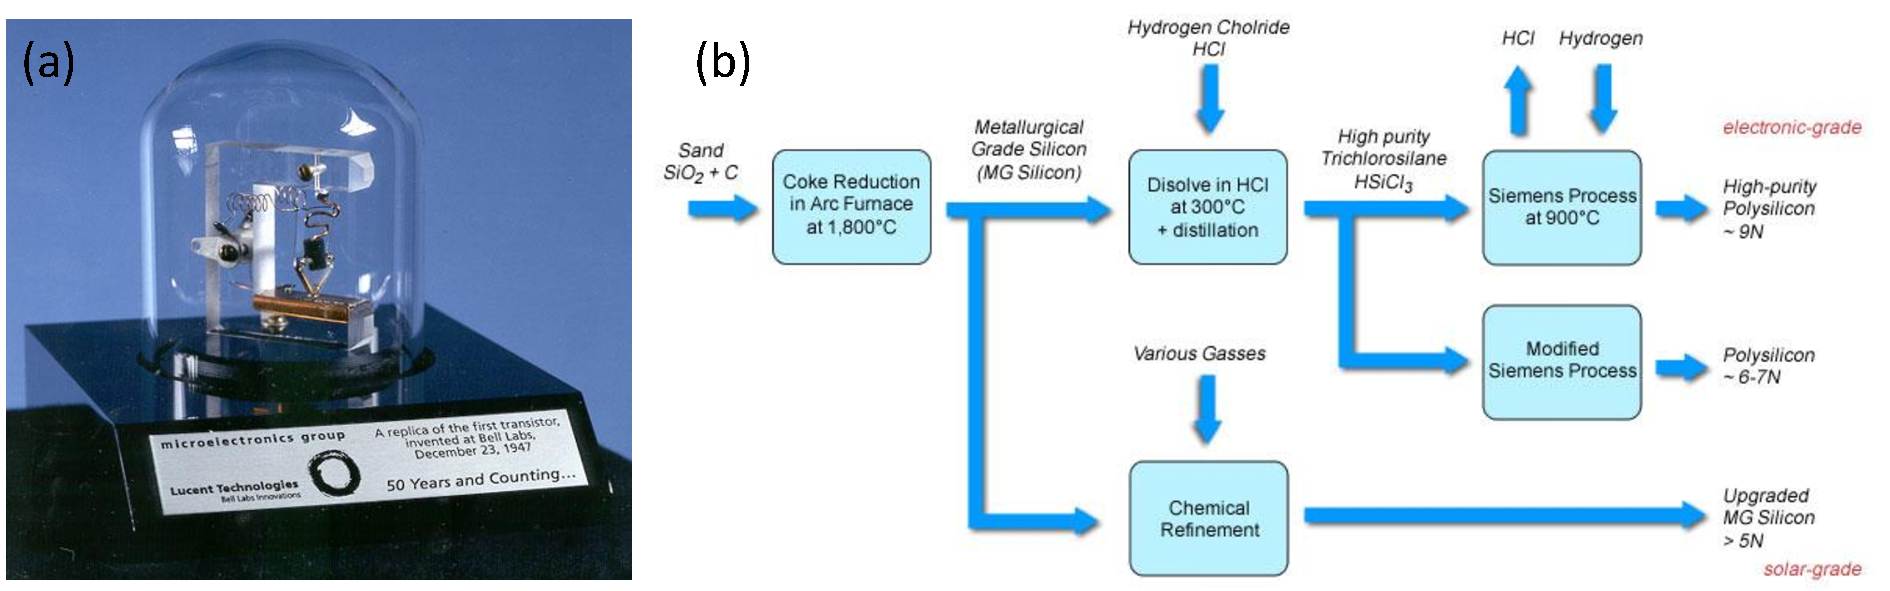
\includegraphics[width=\textwidth]{Fig1}
\caption{(a) Replica of first transistor built in 1946. Reproduced from Ref.\,\cite{Transistor}. (b) Schematic of process required to produce device-grade silicon from starting materials. Reproduced from Ref.\,\cite{Silicon}.}
\label{1Fig1}
\end{figure}

Despite the high stability and carrier mobility in inorganic semiconductors mentioned previous, one major disadvantage is with the processing of such materials. Although Si processing is well-developed, creation of device-grade material still requires many purification steps [Fig.\,\ref{1Fig1}(b)]. Alloys are often produced using vapour or electron-beam deposition, and as such the environmental parameters must be strictly controlled. Layer-by-layer growth can be used for the best quality material, however such processes are costly and time consuming. Current advances in technology require flexible, lightweight and more easily processable semiconductors. 

Although conduction was noted in a mix of aniline and sulphiric acid by Henry Letherby in 1862, research on organic seminconductors began in earnest in the latter half of the 20th century. Polycyclic aromatic compounds were found to form semiconducting charge transfer complexes with halogens in 1954 \cite{Naarmann2002}, and since then much work has been done on developing new molecules and polymers with desired optoelectronic properties, driven by the relative ease with which such molecules can be synthesised. Doping was developed in the 1970s to produce metallic and even superconducting complexes, for example highly conductive oxidised and iodine-doped polyacetylene in 1979 \cite{Shirakawa1977}. Organic semiconductors consist of conjugated molecules, whose overlapping $\pi$ orbitals allow charge transport within the molecule. Given the low production cost, work has be undertaken to produce devices made of organic semiconductors, notably organic photovoltaics, thin film transistors, and light emitting diodes (OLED), probably the most mature organic electronic device as OLEDs have been used mobile phone displays and TVs, with better efficiency and brightness. However problems exist with the manufacturing of such devices, as mass production is not currently optimised for the organic electronic market. More fundamentally, organic semiconductors are less thermally, optically and electrically stable than their inorganic counterparts, leading to lower lifespan of devices. Charge mobility is also lower as hopping between adjacent molecules is required, and lower crystallinity of materials leads to scattering at grain boundaries. 
\begin{figure}[ht]
\centering
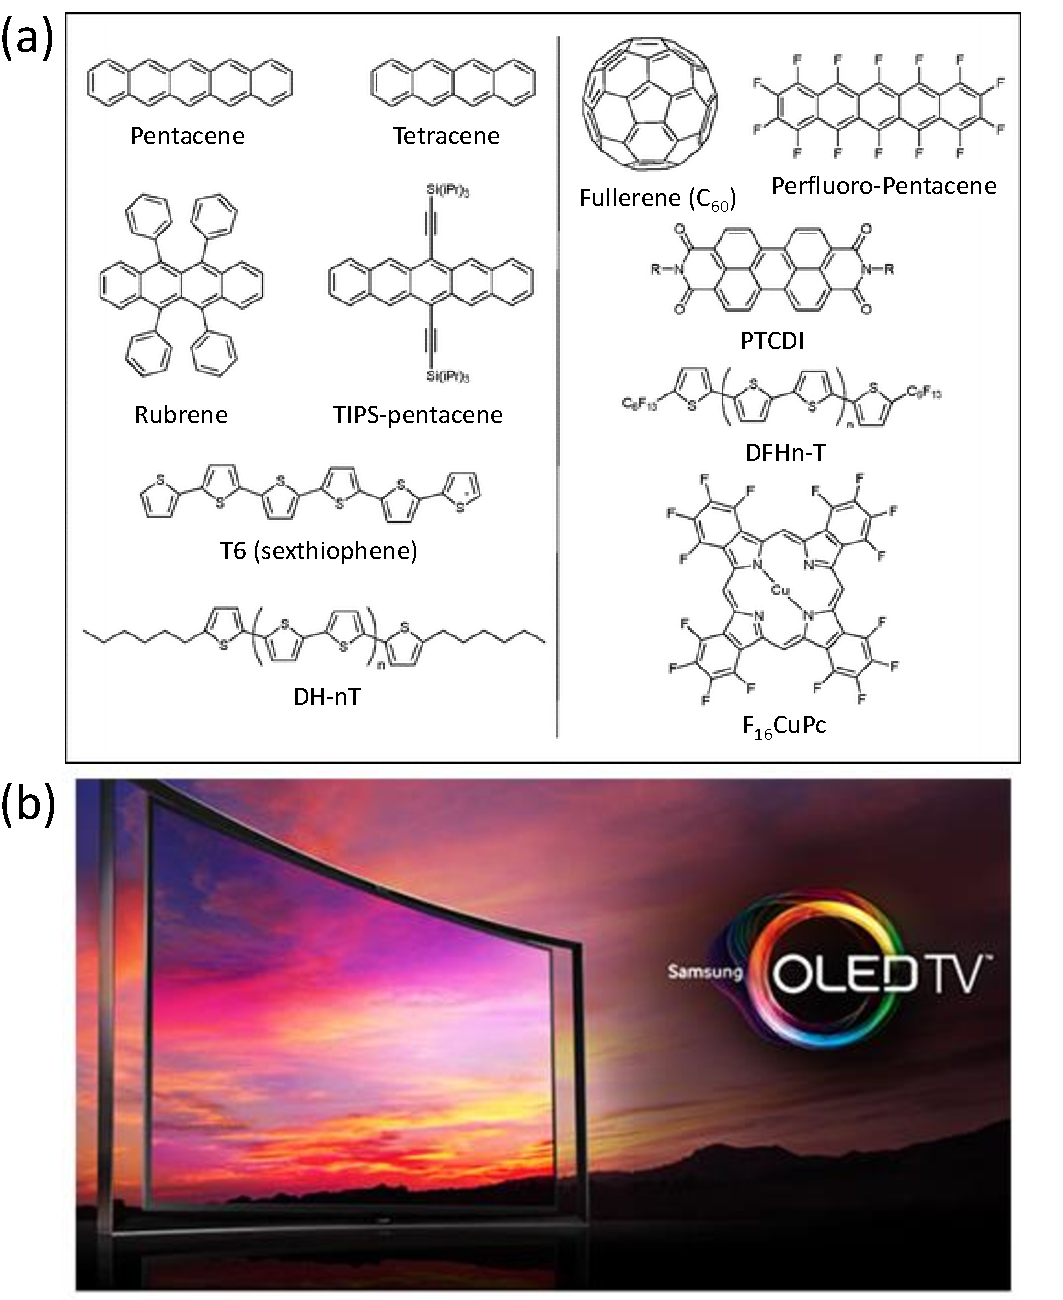
\includegraphics[width=\textwidth]{Fig2}
\caption{(a) Common organic semiconductors, with p-type materials on the left and n-type on the right. Modified from Ref.\,\cite{Miozzo2010}. (b) Samsung curved smart OLED TV. Reproduced from Ref.\,\cite{Samsung}.}
\label{1Fig2}
\end{figure}

A new class of hybrid materials has emerged in the last 20 years. Metal halide based organic-inorganic perovskite semiconductors combine the stability of the inorganic semiconductors with the processability of organic semiconductors. A variety of inorganic frameworks can be formed, all of which are self-assembling. Charge carriers are excited in the inorganic network, and thus share similar optical and electrical properties.

This thesis explores the optical properties of 2D lead iodide-based perovskites, particularly the interactions of perovskite excitons and collective electron oscillations in noble metal nanostructures called surface plasmons. We will first introduce the theory of excitons and review the research on lead iodide perovskites, before exploring the optical properties of surface plasmons. In Chapter 4 we will explore the fabrication of perovskite thin films via spin coating, then study the optical properties of ultrathin perovskite samples produced via exfoliation in Chapter 5. In Chapter 6 we will explore exciton-localised surface plasmon interactions in perovskite-coated metal island structures. Finally in Chapter 7 we look at the coupling between excitons and surface plasmon polaritons in coated plasmonic gratings.
%*****************************************************************************************
%*********************************** Second Chapter **************************************
%*****************************************************************************************

\chapter{Excitons in lead iodide perovskites}

\graphicspath{{Chapter2/Figures/}}

Excitons are neutral quasiparticles consisting of bound electron-hole pairs. Excitons are very important in the emission and absorption spectra of semiconductors, so this Chapter applies basic solid state theory to introduce exciton behaviour in bulk and 2D semiconductors. The rest of the Chapter consists of a brief literature review of exciton effects in organic-inorganic perovskites, from their prevalence in room temperature spectra to potential applications.

\section{Properties of excitons}
Electrons in solids exist in allowed energy bands as a result of mixing and overlap between discrete atomic orbitals. If a electron does not interact with its surroundings (free electron approximation), then it has energy $E=\frac{\hbar^2k^2}{2m_e}$ where $k$ the wavevector of the electron wavefunction and $m_e$ is the rest mass of a free electron. However in reality electrons are affected by positive atomic cores as well as other electrons, giving rise to a deviation from the free electron dispersion, and disallowed energy states (band gaps). Calculating the band structure of even the simplest systems are complex many-body problems, and in general cannot be solved analytically.

However we can still use some basic principles to describe the behaviour of charge carriers in solids. The most important energy bands are the valence band (VB, the highest band occupied by electrons) and the conduction band (CB, the lowest non-occupied band). The difference between the highest energy point of the VB and lowest energy point of the CB is known as the band gap $E_g$. When this gap occurs at the same $k$ point the material is said to have a direct band gap, and if not the band gap is indirect. The Fermi energy $E_F$ is the energy of the highest occupied state at 0\,K, and the behaviour of charge carriers depends on the position of $E_F$ with respect to the conduction and valence bands. Conduction depends on the availability of free electrons in the CB, and in a semiconductor $E_F$ lies in a band gap so there is no conduction at 0\,K. However $E_g$ should be sufficiently small ($\lesssim1$\,eV) so electrons can be thermally excited to the CB and leave behind `holes' in the VB, quasiparticles used to describe an absence of electrons, with charge $+e$ [Fig.\,\ref{2Fig1}(a)]. The behaviour of electrons in response to external forces differs from the free electron value as a result of inter-particle interactions, thus we define the effective electron mass $m_e^*$ as
\begin{equation}
\centering
m_e^{*} = \frac{\hbar^2}{\frac{d^2E}{dk^2}} .
\label{effectivemass}
\end{equation}
The argument also applies to holes, so $m_e^*$ and $m_h^*$ depend on the curvatures of the CB and VB respectively. For the rest of the Chapter the effective mass label $^*$ will be dropped for brevity, however note the free carrier mass can still be used in calculations as an approximation.

\begin{figure}[h!] 
\centering    
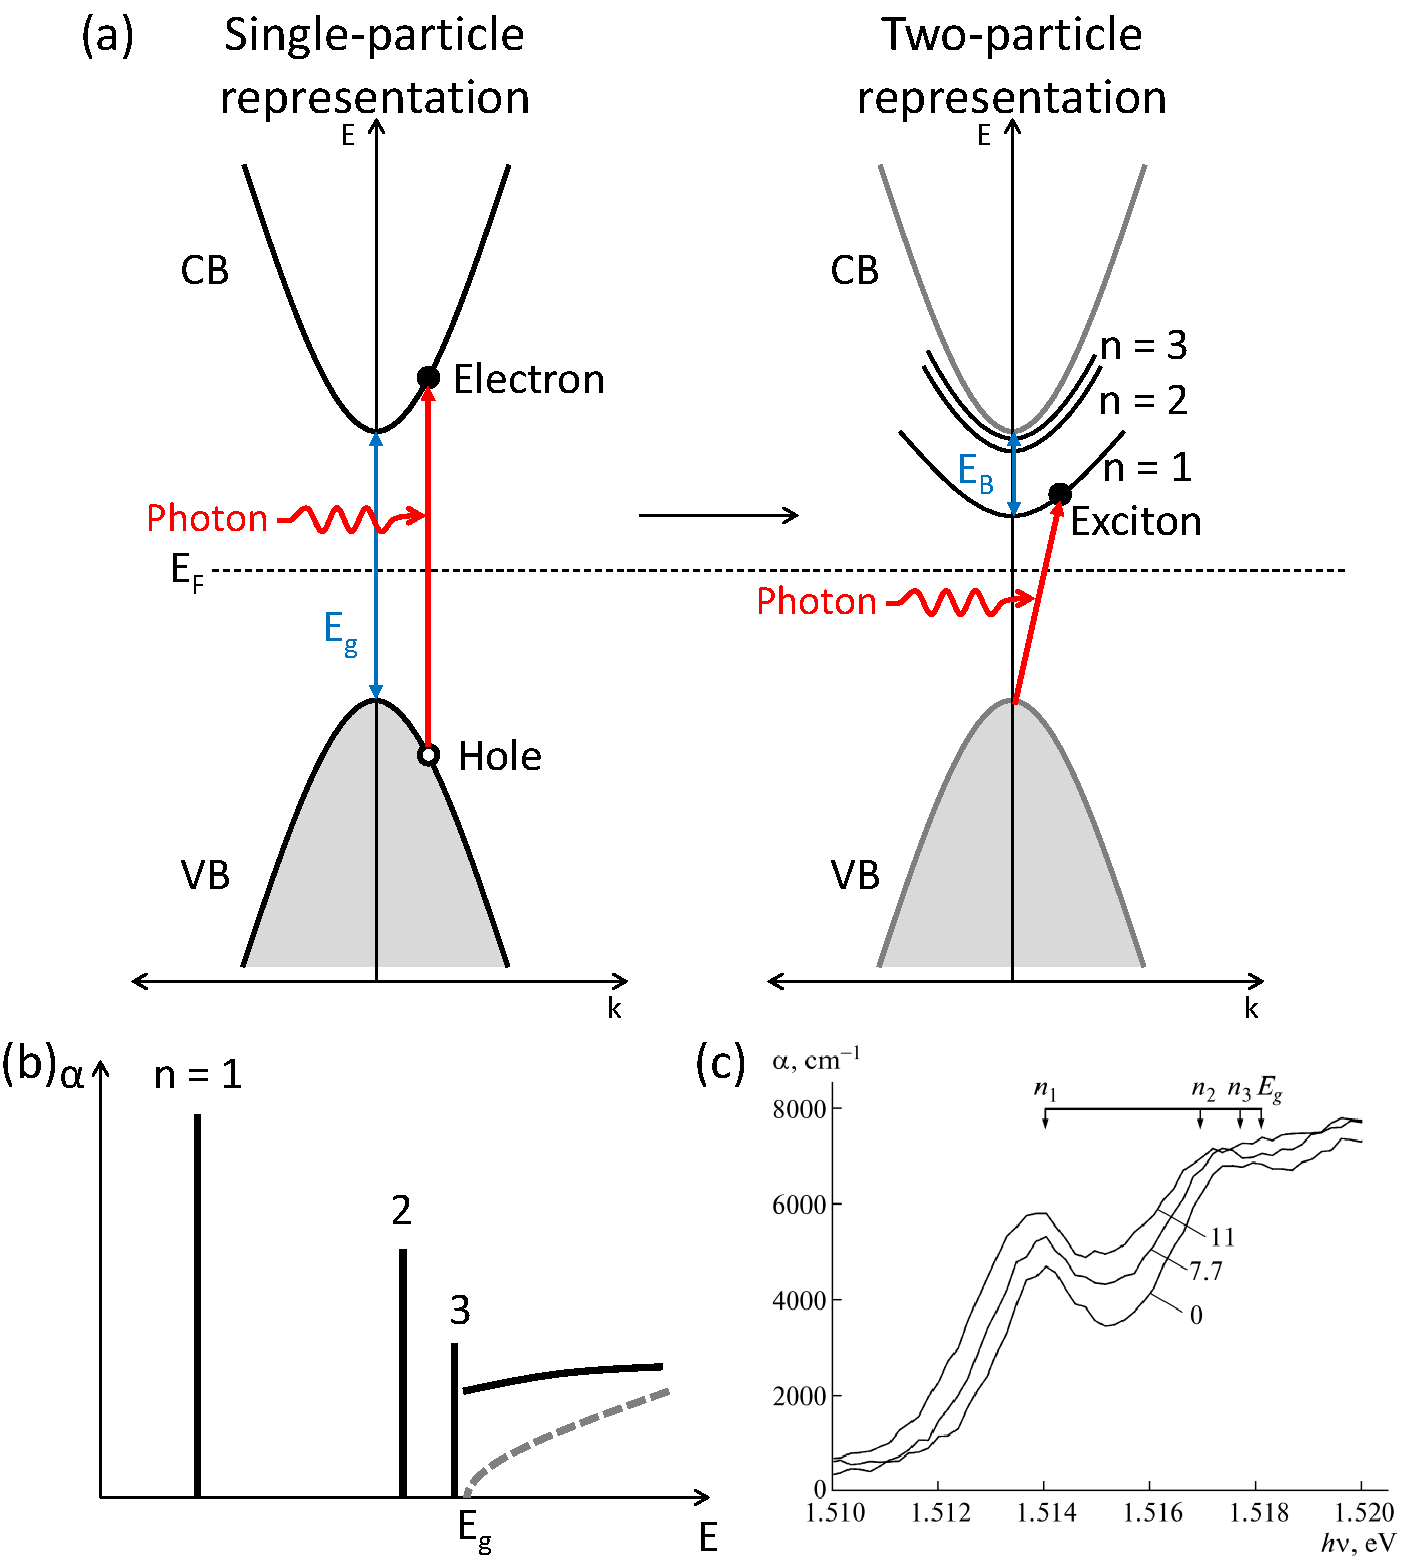
\includegraphics[width=\textwidth]{Fig1}
\caption{(a) (Left) Band structure of a semiconductor, showing the single-particle representation of the excitation of an electron-hole pair via photon absorption. (Right) Two-particle representation of the same system, illustrating exciton energy levels below the CB. (b) Theoretical absorption spectrum of a 3D semiconductor according to Eq.\,\ref{exabs} (not to scale). The dotted line shows the expected band edge absorption without the Sommerfeld factor (see text). (c) Experimental absorption spectrum of GaAs crystal at 1.7\,K, where the excitation power is labelled (W/cm$^2$) \cite{Vaganov2013}.}
\label{2Fig1}
\end{figure}
The attraction between an excited electron and hole binds them together to form a hydrogen-like neutral particle in the crystal. We can therefore use results from the hydrogen atom to find the binding energy $E_B$ and Bohr radius $a_B$ of an exciton:
\begin{subequations}
\label{ex3D}
\begin{align}
E_B &=\frac{\mu e^4}{32\pi^2\epsilon^2\epsilon_0^2\hbar^2n^2} = \frac{R_H}{n^2}\frac{\mu}{\epsilon^2 m_e} \label{exbinding3D}\\
a_B &= \frac{4\pi\epsilon\epsilon_0\hbar^2}{\mu e^4}=a_0\frac{\epsilon m_e}{\mu} \label{exrad3D},
\end{align}
\end{subequations}
where $\mu = (\frac{1}{m_e}+\frac{1}{m_h})^{-1}$ is the effective mass of the exciton, $\epsilon$ is the dielectric constant of the material, and $n$ is the energy level of the exciton ($n=1, 2, 3...$). The Rydberg constant $R_H=13.6$\,eV, and the most probably distance between a proton and electron in the ground state $a_0=0.5$\,\AA\, are defined for the hydrogen atom. Thus a series of exciton energy levels are formed below the lower edge of the CB [Fig.\,\ref{2Fig1}(a)], and the energy of an exciton $E_{ex}$ is given by
\begin{equation}
\centering
E_{ex} = E_g - E_B + \frac{\hbar^2}{2M}(k_x^2+k_y^2+k_z^2),
\label{exenergy}
\end{equation}
where $M = m_e+m_h$ is the total mass of the exciton, and the $k_i$ terms describe its motion in 3D. Eq.\,\ref{exenergy} gives the energy of free excitons that are able to move throughout the crystal, however excitons can be bound to impurities, further lowering their energy.

In inorganic materials, high $\epsilon$ gives rise to $E_B \sim 10$\,meV and $a_B \sim 100$\,\AA, and the so-called Mott-Wannier excitons extend over many unit cells, however due to low $E_B$ the effects can only be observed at low temperature. Conversely organic materials have lower $\epsilon$, such that $E_B \sim 1$\,eV and $a_B \sim 10$\,\AA. These Frenkel excitons are limited to a few unit cells, or one molecule in the case of molecular semiconductors.

Excitons can be created optically by the absorption of photons [Fig.\,\ref{2Fig1}(a)]. In bulk semiconductors, the absorption coefficient $\alpha$ of an exciton depends on the initial ground state $\ket{i}$ (filled VB and empty CB) and final state $\ket{f}$ (one promoted electron), such that
\begin{equation}
\centering
\alpha = \left| \Braket{f | i} \right|^2 \rho(E) ,
\label{exabs}
\end{equation}
where the matrix element $\braket{f | i}$ gives rise to selection rules of possible electronic transitions, and the joint density of states $\rho(E)$ is the number of states per unit energy range between the CB and VB at the photon energy $E$. In 3D $\rho(E)$ has a $\sqrt{E-E_g}$ dependence, however Coulomb interactions lead to an enhancement in the absorption by the Sommerfeld factor, and $\alpha$ is not discontinuous to zero at $E_g$ as expected from Eq.\,\ref{exabs} \cite{Bassu1997}. The theoretical absorption spectrum shown in Fig.\,\ref{2Fig1}(b), with discrete exciton lines decreasing in intensity as $n^{-3}$ \cite{Bassu1997}, and continuous absorption at higher energy due to interband transitions. Experimental data for the absorption of a GaAs crystal at 1.7\,K [Fig.\,\ref{2Fig1}(c)] shows overlap between exciton lines and band edge absorption as a result of the finite exciton peak width $\Gamma_{ex}$. The exciton linewidth is due to a number of factors: firstly homogeneous variables that affect each exciton equally, such as the radiative lifetime of the exciton $\tau_{ex} = \frac{1}{\Gamma_{ex}(0)}$ and collisions with phonons; secondly inhomogeneous factors such as impurities ($\Gamma_{imp}$), whose effects are more localised. Overall this leads to a measured linewidth $\Gamma_{ex}$ that varies with temperature $T$ as
\begin{equation}
\centering
\Gamma_{ex}(T) = \Gamma_{ex}(0) +  \Gamma_{imp}(T) +A_{ac}T + \frac{B_{op}}{\exp{\frac{\hbar\omega_p}{k_B T}}-1},
\label{exwidth}
\end{equation}
where the contribution to phonon collision has been further separated into coupling with acoustic phonons ($A_{ac}$), and interactions with polarised optical phonons of energy $\hbar\omega_p$ \cite{Dammak2009}. 

Once excitons are created, they can annihilate and emit energy in the form of photons. The formation of the charged constituents in excitons causes deformation of the crystal, and as a result of this structural rearrangement the exciton emission is redshifted with respect to absorption, known as the Stokes shift. In general Frenkel excitons in organic semiconductors show larger Stokes shifts as molecules are more easily deformable.

Observations of excitons in optical spectra depends on the coupling between excitons and photons, so exciton peak strength is partly determined by the oscillator strength $f$, given by the matrix element between the exciton and photon wavefunctions. Coupled exciton-photon states are known as exciton-polaritons. Non-propagating solutions give rise to longitudinal excitons with frequency $\omega_L$, while travelling solutions produce transverse excitons with frequency $\omega_T$. The longitudinal-transverse splitting $\omega_{LT} = \omega_L - \omega_T$ is again related to the coupling between excitons and photons, with $f \sim \sqrt{\epsilon_B} \omega_{LT}$, where $\epsilon_B$ is the background dielectric constant of the material without excitonic contributions.

\section{Excitons in 2D systems}
\label{sec:ex2D}
Exciton motion can be confined to 2D in quantum well (QW) systems, where a well material is sandwiched between barrier layers with higher $E_g$. If the well and barrier layers are periodically arranged then a multiple quantum well (MQW) or superlattice is formed. Four types of band alignment can be achieved [Fig.\,\ref{2Fig2}(a)]: in type I structures potential steps appear in both the VB and CB, thus confining both electrons and holes to the well region. In type II QWs band edges of the barrier layers are shifted in one direction with respect to the well, creating a staggered band alignment where the electrons are confined to the well and holes to the barrier region. In the most extreme case the barrier VB is above the well CB, creating a type II broken-gap arrangement. Type III QWs occur when a semimetal (with a small overlap between the VB and CB) is used as the well. For the rest of this section only type I QWs will be considered.

Type I QWs can be formed from a variety III-V composite materials, for example GaAs/AlGaAs, GaAs/AlAs or GaAs/GaP. In designing a QW system, one must consider the lattice constants of the materials in question as well as the electronic band structure. A large lattice mismatch will cause strain in the layers, and the growth will not be epitaxial, i.\,e.\, there will not be a well-defined crystal structure throughout the layer. The AlAs/GaAs system has good lattice matching, or alternatively a ternary alloy can be used to reach the lattice constant needed. It is also possible to use materials that can adapt to the local lattice constant up to a critical thickness despite strain. In general these inorganic QWs are grown atomically layer-by-layer, either using molecular beam epitaxy (MBE) or metalorganic chemical vapour deposition (MOCVD), where the relevant atoms are deposited onto the substrate either in the gas phase or via a molecular beam. The stoichiometric mix of relevant atoms must be carefully controlled during fabrication to create the correct structures. 

The layered structure of a QW confines carrier motion in the direction of layer growth, thus creating a 2D system. If the width of the well layer $L$ is on the order of the electron de Broglie wavelength ($\sim10$\,nm), then then carriers are essentially trapped in a finite potential well and we observe wave-like effects such as the creation of discrete energy levels in which electrons/holes can reside. Using the results for a particle in an infinite well for simplicity, the energy $E_u$ of allowed states are
\begin{equation}
\centering
E_u = \frac{\hbar^2}{2m} \left(\frac{u\pi}{L}\right)^2 ,
\label{particleboxenergy}
\end{equation}
where $m$ the mass of the carrier, and the index $u$ labels the energy level. Instead of the VB/CB, we find instead a series of minibands with different energies [Fig.\,\ref{2Fig2}(b)]. The absorption spectrum of QW systems can still be calculated using Eq.\,\ref{exabs}, however the orthogonality of eigenstates means that transitions from state $\Ket{u_1}$ in the VB to $\Ket{u_2}$ in the CB are only allowed if $u_2-u_1=0$. The joint density of states $\rho(E)$ is step-like in 2D, again with the Sommerfeld factor enhancing absorption [Fig.\,\ref{2Fig2}(c)].
\begin{figure}[h!] 
\centering    
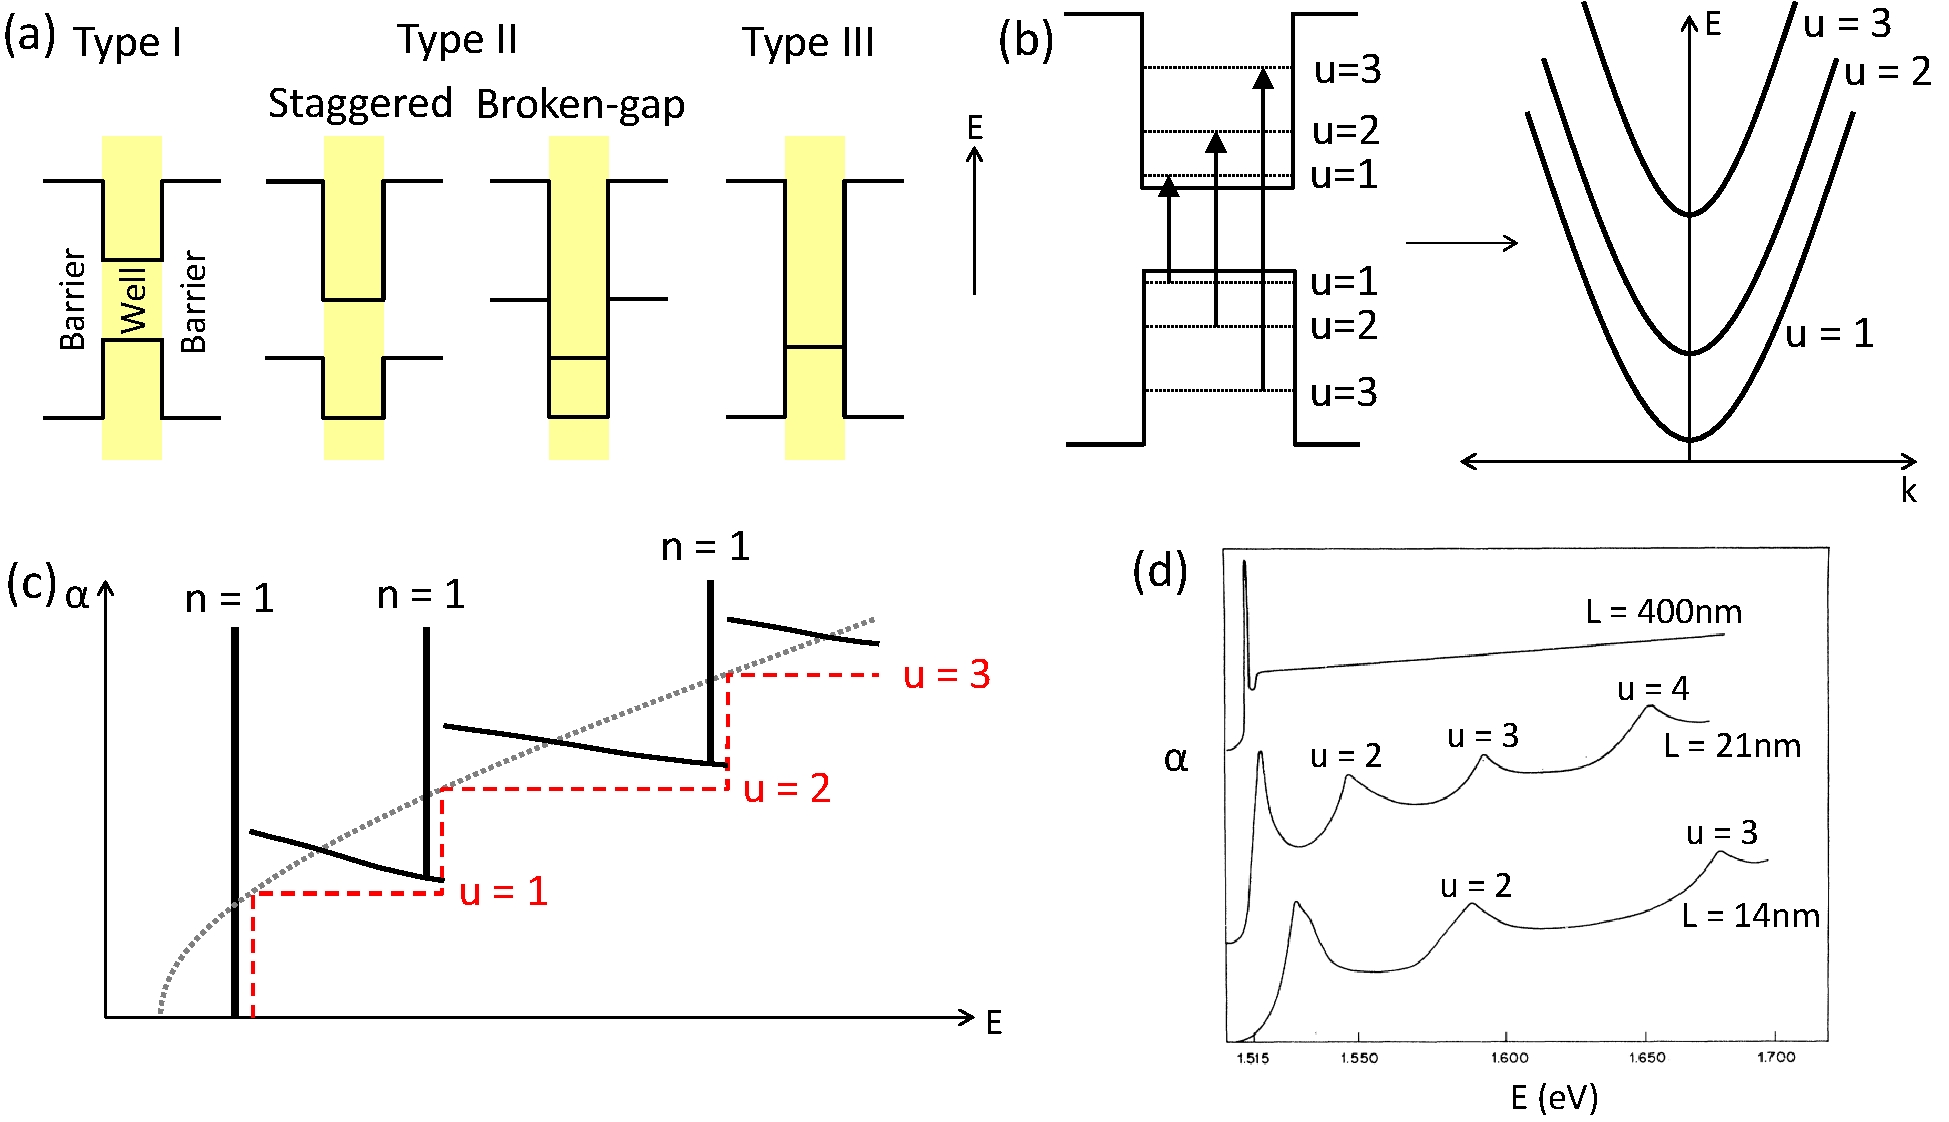
\includegraphics[width=0.53\textwidth]{Fig2}
\caption{(a) Schematic of quantum well band alignments. (b) Allowed transitions for electrons in a quantum well (left) and the resultant miniband structure (right). (c) Theoretical absorption spectrum of a 2D quantum well according to Eq.\,\ref{exabs} (black lines). The band edge absorption in 3D (grey dotted line) and 2D (red dashed line) are both shown with the Sommerfeld factor. (d) Experimental absorption spectrum of GaAs/Al$_{0.2}$Ga$_{0.2}$As quantum wells with the labelled well width $L$ at 2\,K. Only the $n=1$ exciton peaks (labelled ex) are observed, but the minibands $u$ are labelled. Adapted from Ref.\,\cite{Dingle1974}.}
\label{2Fig2}
\end{figure}

Exciton bands exist below each of the minibands, and in order to find $E_B$ we use the results for a hydrogen atom in 2D, such that
\begin{equation}
\centering
E_B =\frac{\mu e^4}{32\pi^2\epsilon^2\epsilon_0^2\hbar^2\left(n+\frac{1}{2}\right)^2} = \frac{R_H}{\left(n+\frac{1}{2}\right)^2}\frac{\mu}{\epsilon^2 m_e} .
\label{exbinding2D}
\end{equation}
Therefore the energy of the exciton bands $E_{ex}$ can be described by
\begin{equation}
\centering
E_{ex} = \Delta E_u - E_B + \frac{\hbar^2}{2M}(k_x^2+k_y^2) ,
\label{exenergy2D}
\end{equation}
where $\Delta E_u$ describes the transition between energy levels $u$ in the CB and VB. The expected absorption spectrum of a QW structure is shown in Fig.\,\ref{2Fig2}(c), while experimentally measured spectra for GaAs/Al$_{0.2}$Ga$_{0.8}$As QWs are shown in Fig.\,\ref{2Fig2}(d). Note how the change in $L$ affects the allowed $\Delta E_u$, with $L=400$\,nm essentially appearing as a 3D system.

We can see from Eq.\,\ref{exbinding2D} that the reduction in dimensionality leads to a factor of 4 enhancement in $E_B$ for the $n=1$ state, so exciton effects should be observable at higher temperatures in QWs. Similarly $a_B$ is reduced by a factor of 2 in QWs as a result of confinement. For this reason is it often said that excitonic effects are stronger in QWs, with increased overlap between the electron and hole wavefunctions.

\section{Properties of PbI perovskites}
%Organic-inorganic metal halide perovskite semiconductors can combine the distinct properties of its organic (ease of processing, structural diversity, plastic mechanical properties) and inorganic (band structure variability, electrical mobility, thermal and mechanical stability) constituents into one composite.
\subsection{Structure and bonding}
Metal halide \ce{RNH3MZ3} organic-inorganic semiconductors are based on the \ce{ABX3} perovskite crystal structure [Fig.\,\ref{2Fig3}(a)], consisting of a corner-sharing octahedra network of halogen atoms Z (most commonly I, Br or Cl) with a metal atom M in the centre of each octahedron (\ce{+2} valence metals such as Pb, Sn, Cd, Zn, Cu, or Co). Organic mono-ammonium molecules \ce{RNH3} hydrogen bond to halogen atoms and reside in the interstices between octahedra [Fig.\,\ref{2Fig3}(b)], and as a result only very short molecules are used, the most common of which is \ce{CH3NH3}. The band gaps of such semiconductors can be engineered by changing the metal and halogen composition, and recently lead halide-based semiconductors have been used as a light absorbing layer in solar cells, producing efficiencies of up to 16\%, and there is currently a drive to find lead-free alternatives for wider use \cite{Lee2012, Heo2013, Liu2013, Hao2014}. A change in the stoichiometric mix of organic and inorganic constituents results in the formation of lower dimension structures, for example 2D layered systems, or 1D inorganic wires \cite{Nagami1996, Fukumoto2000, Fujisawa2004, Pradeesh2010}. From here we will focus on <100> oriented 2D lead iodide (PbI) perovskites \cite{Mitzi2001}.

The self-assembled structure of 2D hybrid PbI perovskites with formula \ce{(RNH3)2PbI4} are shown in Fig.\,\ref{2Fig3}(c), and consist of alternating layers of corner-sharing \ce{PbI6} octahedra and interdigitating \ce{RNH3} molecules (where R is an organic moiety). The organic molecules have larger $E_g$ (\sim6$\,eV) than the inorganic layers ($\sim3$\,eV), and form a type I MQW structure \cite{Ishihara1994, Pradeesh2009b}. The width of the QW (PbI octahedra) is $\sim6.5$\,\AA~\cite{Ishihara1989}. The bonding in inorganic layers is primarily ionic as Pb-I distances are more comparable to the sum of ionic radii \cite{Mousdis2000}. Inorganic sheets are sandwiched between layers of organic molecules via hydrogen bonding between $\textrm{NH}_3$ groups and I atoms, while the van der Waals or aromatic-aromatic interactions that bind organic molecules together can (de)stabilise the perovskite structure \cite{Mitzi2001a}. Like other layered materials such as graphene or transition metal dichalcogenides, it is possible to break these van der Waals bonds and cleave the structure and produce thinner samples.
\begin{figure}[h!] 
\centering    
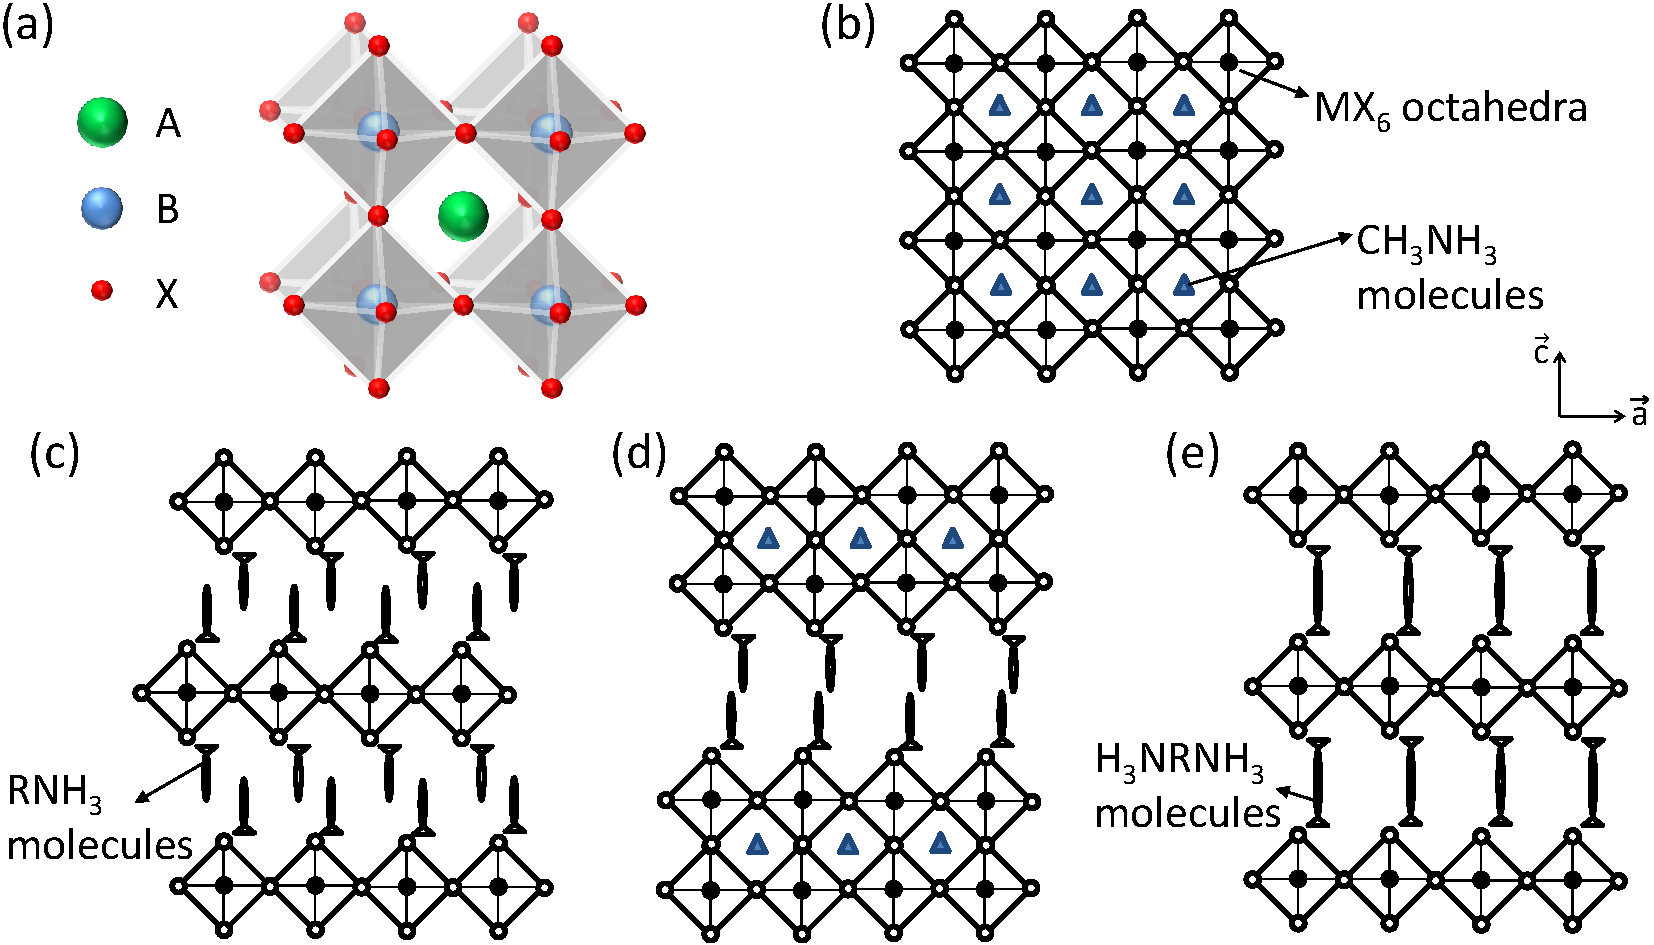
\includegraphics[width=\textwidth]{Fig3}
\caption[Crystal structure of (a) \ce{ABX3} perovskite, (b) 3D hybrid perovskite, (c) 2D hybrid perovskite, (d) 2D multilayered perovskite, and (e) 2D diammonium perovskite viewed along the crystallographic $\vec{b}$ axis.]{Crystal structure of (a) \ce{ABX3} perovskite, (b) 3D hybrid perovskite \ce{(CH3NH3)PbI3}, (c) 2D perovskite \ce{(RNH3)2PbI4}, (d) 2D multilayered perovskite \ce{(RNH3)2(CH3NH3)Pb2I7}, and (e) 2D diammonium perovskite \ce{(H3NRNH3)PbI4} viewed along the crystallographic $\vec{b}$ axis.}
\label{2Fig3}
\end{figure}

There are two main orientations for consecutive inorganic layers: eclipsed layers produce a monoclinic structure, while staggered layers produce an orthorhombic structure \cite{Billing2006}. The orientation is chosen to accommodate organic molecules in the structure. Phase transitions from the orthorhombic phase to the monoclinic phase will lead to a halving of the $c$ lattice parameter due to increased symmetry \cite{Billing2008}.

There are only a few limits on the organic molecule \ce{R} in the structure. The cross section of the molecule should be small enough to fit into the interlayer space between four adjacent octahedra ($\lesssim 40$\,\AA$^2$) \cite{Mitzi2001a}. However their lengths are not constrained so long as the intermolecular forces are strong enough to hold the structure together. Systems with aromatic molecules tend to be better organised with more crystallinity since such molecules allow for self-assembly using stronger aromatic-aromatic interactions, conversely large organic groups will hinder self assembly and reduce crystallinity \cite{Zhang2009}. In general very simple organic molecules are used, for example those based on simple alkane chains (($\textnormal{C}_n\textnormal{H}_{2n+1}$\ce{NH3)2PbI4}, C$_n$PI hereafter), ring structures (\ce{(C6H9NH3)2PbI4}, CHPI), or aromatic molecules (\seqsplit{\ce{(C6H5C2H4NH3)2PbI4}}, PAPI). However more complex organic molecules can be incorporated, for example optically active ligands \cite{Billing2006, Teshima2003} and fullerene derivatives \cite{Kikuchi2005, Kawabata2009}. 

The basic 2D layered structure can be varied in a series of ways. For instance the width of QWs	can be varied by extending the inorganic sheets to contain multiple layers of \ce{PbI6} octahedra (\ce{(RNH3)2(CH3NH3)}$_{n-1}\textnormal{Pb}_n\textnormal{I}_{3n+1}$) [Fig.\,\ref{2Fig3}(d)] \cite{Calabrese1991}. Another is with the use of diammonium organic molecules, which can hydrogen bond to two consecutive inorganic layers, therefore eliminating the need for van der Waals interactions between the interweaving molecules (\ce{(H3NRNH3)PbI4}) [Fig.\,\ref{2Fig3}(e)].

\subsubsection{Phase transitions in $\textrm{C}_n$PI}
\label{sec:Cnphases}
Four main phases of $\textrm{C}_n$PI perovskites have been identified. For temperatures $< -30^{\circ}$C (phase I), the crystal exhibits twinning so atomic positions cannot be determined. Between $-30$ and $15^{\circ}$C  (phase II), organic chains are ordered with uniform tilting angle. The structure then undergoes a pre-melting transition, leading to dynamic rotational disorder of $\textrm{NH}_3$ groups and a small decrease in the lattice parameter $c$ \cite{Barman2003}. Between $\sim 15$ and $65^{\circ}$C (phase III), organic chains show much more conformational disorder and become tilted at different angles, leading to a large increase in $c$, and thus an increase in volume since no lateral motion occurs \cite{Barman2003}. Above $65^{\circ}$C (phase IV), organic chains appear to be `melting' \cite{Ishihara1990, Xu1991, Ishihara1989}. Simulations show that after the melting transition alkyl chains are no longer all-trans, and the introduction of gauche defects leads to a shortening of the chain and an increase in its effective cross-sectional area. Conflicting demands of close packing that optimise dispersive interactions and the larger area required by conformationally disordered chains can no longer be met by a uniformly tilting arrangement, and the non-uniform tilt allows for increased space for individual chains \cite{Naik2010}. Changes in conformation during phase transitions also cause a spatial shift in the coupling between $\textrm{NH}_3$ groups and inorganic octahedra \cite{Pradeesh2009}. In order to accommodate the changes in alkyl chains, $\textrm{PbI}_6$ octahedra can undergo two types of structural change: they can tilt perpendicular or parallel to the inorganic sheets. During perpendicular tilting octahedra are tilted with respect to each other, whereas parallel tilting leads to an overall corrugation of inorganic layers \cite{Billing2008}. For $\textrm{C}_{12}$-, $\textrm{C}_{14}$-, $\textrm{C}_{16}$-, and $\textrm{C}_{18}$PI phase III is orthorhombic with staggered inorganic sheets, and phase IV is monoclinic with eclipsed inorganic sheets \cite{Billing2008}.    
%\begin{figure} [h!]
%\centering
%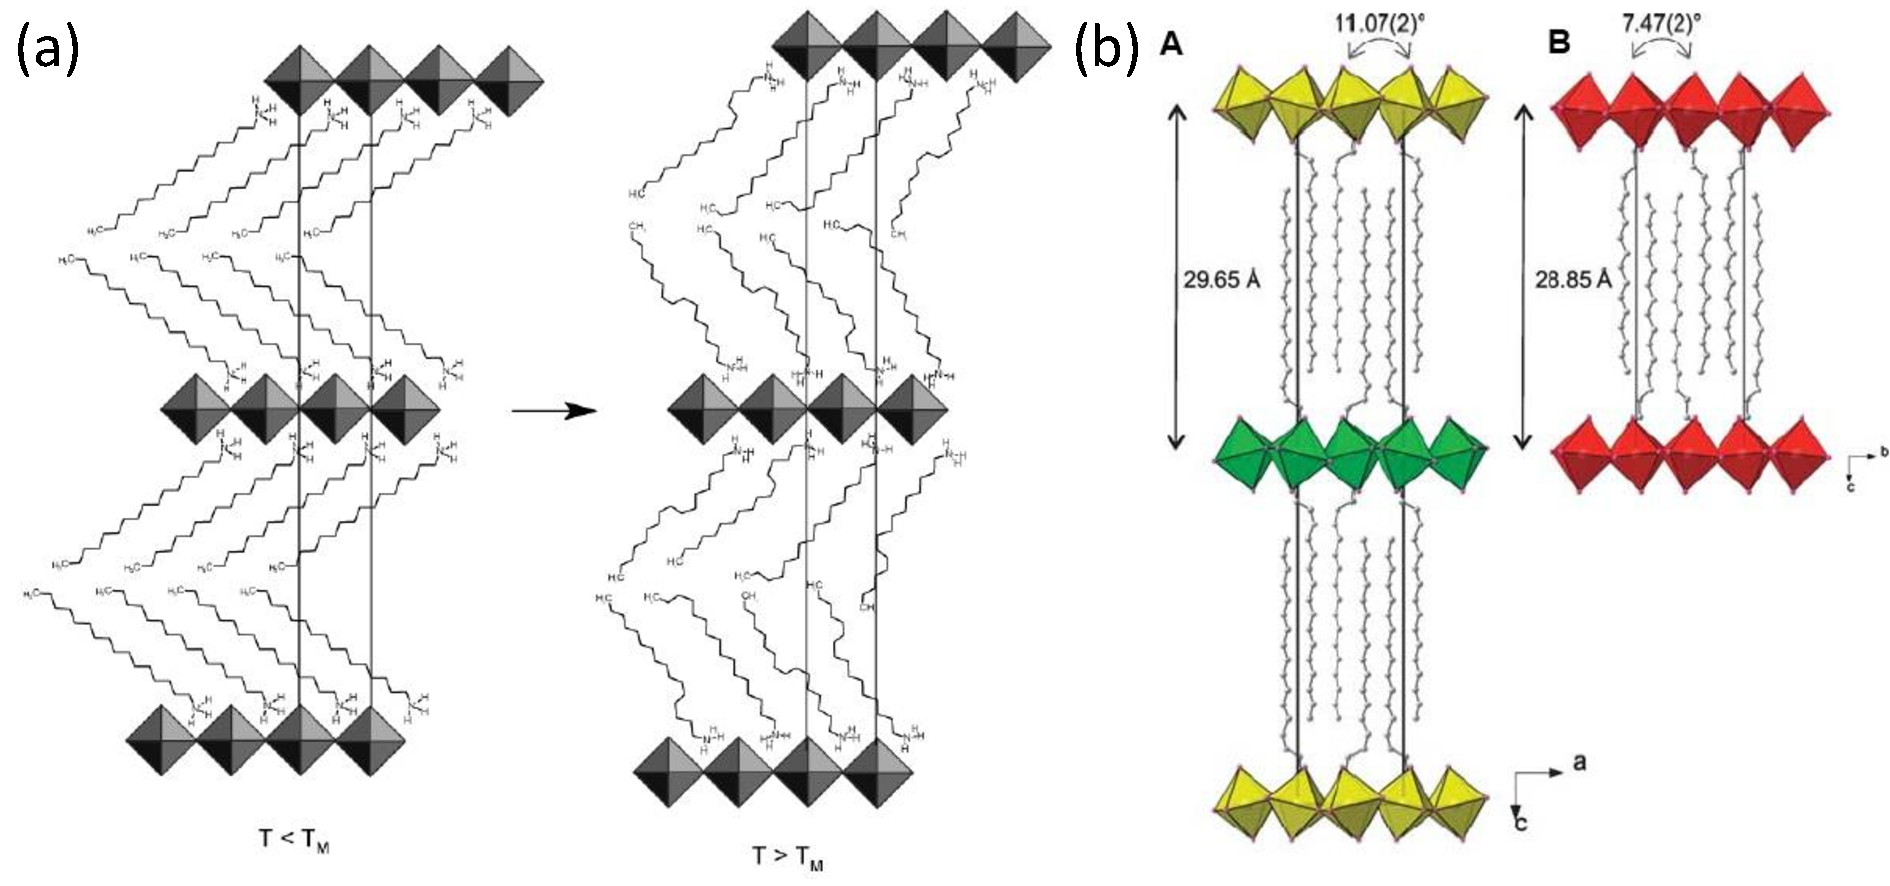
\includegraphics[width=\textwidth]{Fig4}
%\caption {(a) Structure of $\textrm{C}_{n}$PI ($n$=12, 14, 16, 18) before (A) and after (B) the pre-melt transition. A is orthorhombic, and B is monoclinic so the lattice parameter $c$ is halved. (b) Schematic of the melting transition in $\textrm{C}_{10}$PI. Below the melting temperature $T_M$, the chains adopt an all-trans conformation (no gauche defects \cite{Naik2010}) with a well defined tilt angle of around $55^{\circ}$ \cite{Venkataraman2002, Venkataraman2002a}. Above $T_M$, alkylammonium chains are conformationally disordered with different tilt angles. (a) Reproduced from Ref.\ \cite{Billing2008}, (b) from \cite{Barman2003}.}
%\label{2Fig4}
%\end{figure}

The switching between orthorhombic and monoclinic phases can be controlled by parameters other than temperature. Pradeesh \textit{et al.}\ showed that the phases present in spin coated films of $\textrm{C}_{12}$PI depend on the thickness of the sample, as well as ageing effects. They postulated that this is due to strain, where high strain in thicker samples favours the flatter orthorhombic phase. Ageing effects, where a sample in the monoclinic phase gradually shifted to the orthorhombic phase, can be stopped by annealing or capping with poly(methyl methacrylate) (PMMA) \cite{Pradeesh2009}.

\subsection{Fabrication and processing techniques}
\subsubsection{Silica-gel method}
An aqueous solution of Pb($\textrm{CH}_3 \textrm{COO)}_2$, $\textrm{C}_n\textrm{H}_{2n+1}\textrm{NH}_2$, $\textrm{CH}_3$COOH, and $\textrm{Na}_2\textrm{SiO}_3$ is prepared in a test tube, and becomes a gel after approximately one week. At this point an aqueous solution of KI is poured into the gel and the $\textrm{I}^-$ ions diffuse slowly into the gel to form $\textrm{C}_n$PI single crystals. About a month after the introduction of KI, platelet-like crystals form, approximately $2\times 2\times 0.1$~mm in size. However crystals for perovskites where $n=4,6$ cannot be produced using this method \cite{Ishihara1990}.

The silica-gel method allows multiple components to be mixed in solution on a nanometre scale, which can produce very homogeneous materials. The technique can also be used to make thin films by dissolving the raw ingredients in a suitable solvent (e.\,g.\,an alcohol) that is fast gelling and drying. The necessary condensation reaction and solvent evaporation will take place after the solution is applied to a substrate, leaving behind a wet gel film that can be heated to produce a dry film, but in order to avoid cracking the wet film should generally be less than 1\,$\mu$m thick. Thin gel films are usually amorphous, but surfactants on the substrate can help with assembly and annealed films are generally crystalline \cite{Mitzi2001b}.

\subsubsection{Solution crystal growth}
\label{sec:solutiongrowth}
The silica-gel method is time intensive, therefore crystals of a similar or larger size are more commonly produced from solution. Pb$\textrm{I}_2$, R$\textrm{NH}_2$ and HI are usually mixed in stoichiometry and left for solvent evaporation \cite{Kitazawa1996, Tang2001, Ishihara1994}. The basic reaction scheme is \ce{2RNH3 + 2HI + PbI2 -> (RNH3)2PbI4}. After around one week single crystals form, although the rate of evaporation can be controlled to change the morphology of crystals \cite{Cheng2010}. The difficulty lies in finding solvents that will dissolve both the inorganic and organic parts of the perovskites, and examples include acetone \cite{Hong1992}, dimethylformamide (DMF) \cite{Kitazawa1996}, and HI \cite{Barman2003}. If the evaporation is less controlled, this method can be used to create perovskite powder, which can later be dissolved in a suitable solvent and used in spin coating.

\subsubsection {Spray pyrolysis/drying}
Spray pyrolysis produces particles when misted streams of precursor solution are introduced to a furnace. Multicomponent particles can be prepared due to microscale reactions inside the micrometre-sized droplets, and new phases with narrow size distributions and non-agglomeration can be obtained rapidly after solvent evaporation and as a result of high temperature and inert gas streams inside the furnace reactor \cite{Cheng2005}. 

A precursor solution of stoichiometric quantities of $\textrm{PBI}_2$ and $\textrm{C}_6\textrm{H}_5\textrm{C}_2\textrm{H}_4\textrm{NH}_3\cdot\textrm{HI}$ in tetrahydrofuran (THF) is used to prepare PAPI powder. From scanning electron microscope (SEM) images the powder particles are $\sim 1\, \mu$m in size, however XRD data indicate the structure is less organised than PAPI prepared by other methods, e.\,g.\, spin coating. The photoluminescence (PL) spectrum of PAPI powder shows a strong exciton peak, indicating the formation of the required layered structure, however the wavelength is shifted by around 5\,nm, likely due to distortion of PbI sheets \cite{Cheng2005}.

A similar technique of spray drying can be used to produce perovskite nanoparticles. The precursor solution is prepared by bubbling a flow of dry HI into a dry ethereal solution of organic amine. Drying droplets (initial mean diameter $\sim 35\,\mu$m) are carried from the aerosol generator by dry air into an evaporation chamber at $250^{\circ}$C. Dried nanoparticles created using this method are mostly spherical, but with a large size distribution ($50-500$\,nm diameter; average $60\pm10$\,nm). The perovskite crystallises at the edge of the particle while the centre is depleted, therefore larger nanoparticles are hollow, while smaller particles are denser due to their fast drying rate. XRD data indicate the nanoparticles are crystalline, with a small redshift of a few nanometres in exciton PL caused by strain. The nanoparticles are also fairly photo-stable, with a drop in PL intensity of around 30-50\% after illumination of 1\,hour \cite{Audebert2009a}.

\subsubsection {Langmuir-Blodgett technique}
The Langmuir-Blodgett (LB) technique uses a movable barrier to apply pressure to a monolayer of molecules at a liquid-gas interface. When molecules are close enough van der Waals forces can create close packing, thus forming a thin film [Fig.\,\ref{2Fig6}(a)] \cite{Mitzi2001b}. Era \textit{et al.}\ used LB to create thin films of $(\textrm{C}_{22}\textrm{H}_{45}\textrm{NH}_3)_2\textrm{PbBr}_4$. The long chain ammonium bromide ($\textrm{C}_{22}\textrm{H}_{45}\textrm{NH}_3$Br) is spread on an aqueous subphase containing Pb$\textrm{Br}_2$ and $\textrm{CH}_3\textrm{NH}_3$Br from a chloroform and DMF solution. The monolayer is then pressed to a surface pressure of 30\,mN$\textrm{m}^{-1}$, then deposited on a hydrophobidised fused quartz substrate. Layer-by-layer deposition of LB films allows control over the film thickness. Films show strong exciton absorption peaks, with linear increase in the absorption intensity for each additional layer [Fig.\,\ref{2Fig6}(b)] \cite{Era2000}.
\begin{figure} [h!]
\centering
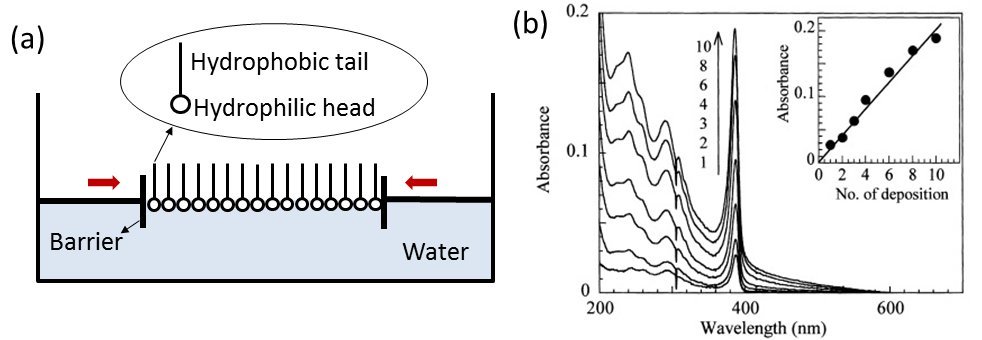
\includegraphics[width=\textwidth]{Fig6}
\caption{(a) Schematic of Langmuir-Blodgett setup and the amphiphilic nature of molecules ordered on the water-air interface. (b) Absorption spectra of LB film obtained using the labelled number of depositions, and exciton absorbance intensity against the number of depositions (inset) \cite{Era2000}.}
\label{2Fig6}
\end{figure}

\subsubsection{Intercalation}
Perovskite films can be formed by the intercalation of organic molecules into an inorganic framework. Pb$\textrm{I}_2$ films are deposited onto substrates by vacuum deposition or spin coating, and a solution of organic ammonium iodide prepared. The Pb$\textrm{I}_2$ covered substrates are dipped in the iodide solution and dried. The resulting films have the same properties as films created using other methods \cite{Liang1998}, and the film thickness is controlled by the initial Pb$\textrm{I}_2$ thickness. In the case of CHPI only 10\,s is needed to complete intercalation for a film $\sim70$\,nm thick \cite{Pradeesh2009a}.

A similar dipping method has been used to make thin films of the diammonium perovskite \mbox{\ce{(H3NC12H25NH3)PbI4}}. Hydrophilic quartz substrates are alternately dipped in organic diammonium iodide and \ce{PbI2} solutions, with care taken to remove excess reactants after each step. The procedure can be repeated as needed to create multilayers of self-assembled quantum wells and control the film thickness \cite{Matsui2002}.

Gaseous intercalation has also been demonstrated by Era \textit{et al.}. A 20\,nm thick film of Pb$\textrm{I}_2$ is vacuum deposited on a quartz substrate, then exposed to vaporised organic ammonium iodide ($\textrm{C}_6\textrm{H}_5\textrm{C}_2\textrm{H}_4\textrm{NH}_3\textrm{I}$). Both XRD and absorption confirm the formation of PAPI, although in XRD signatures of Pb$\textrm{I}_2$ can still be seen \cite{Era1998}.

Recently in-situ measurements on liquid-phase intercalation has shown that the process begins from the top surface of the \ce{PbI2} film, and proceeds parallel to the $\vec{c}$ axis. Organic molecules attach to the top \ce{PbI2} layer as terminal groups, and transform the edge-sharing PbI octahedra into a corner-sharing network. Interstices are opened for the diffusion of organic molecules, which interact with the bottom surface of the same layer, thus converting the \ce{PbI2} layer into full 2D perovskite monolayer. Further diffusion continues intercalation for subsequent layers [Fig.\,\ref{2Fig7}]. This process requires a non-polar solvent that will not compete with the hydrogen bonding between the inorganic and organic constituents, and an optimum organic iodide concentration exists due to steric hindrance of neighbouring molecules \cite{Ahmad2014}.
\begin{figure} [h!]
\centering
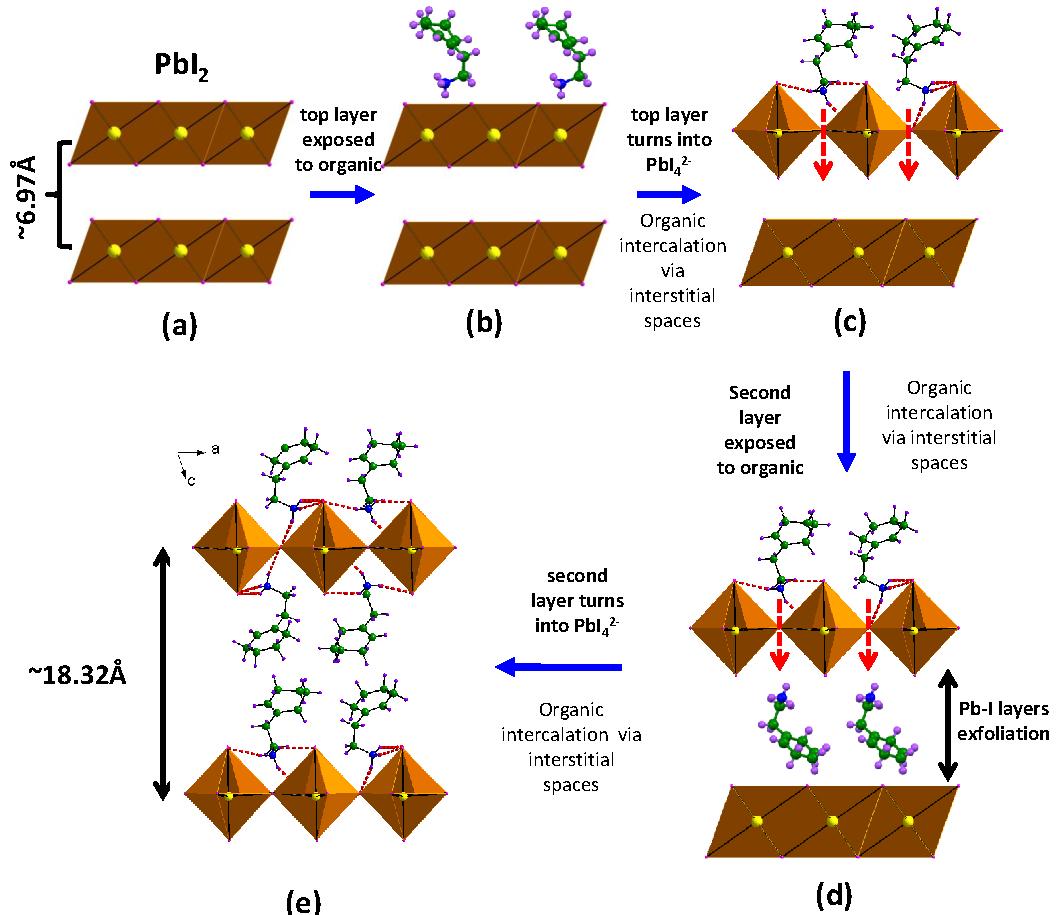
\includegraphics[width=\textwidth]{Fig7}
\caption{Molecular dynamics for the liquid-phase intercalation of organic ammonium iodide molecules into \ce{PbI2} film.}
\label{2Fig7}
\end{figure}

\subsubsection{Dual-source vacuum deposition}
PAPI films can be created using a dual-source vacuum deposition method, where both Pb$\textrm{I}_2$ and $\textrm{(C}_6\textrm{H}_9\textrm{C}_2\textrm{H}_4\textrm{NH}_3)\textrm{I}$ are deposited simultaneously on a quartz substrate. The created films show the same sharp exciton absorbance peaks as films and crystals created by other methods [Fig.\,\ref{2Fig8}], however the films are disordered as XRD data show no peaks at high $\theta$. The growth of the layered perovskite structure appears to occur in the solid phase on the substrate \cite{Era1997}. As the organic ammonium halide may dissociate into an amine and HI, care needs to be taken with choice of evaporation rates, or else films can be multiphasic, disordered or defective \cite{Mitzi1999}.
\begin{figure}[h!]
\centering
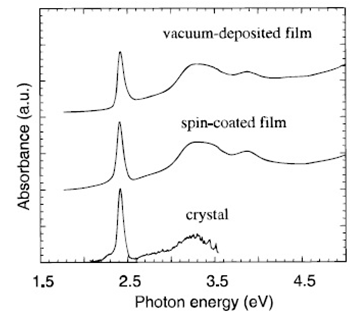
\includegraphics[width=0.6\textwidth]{Fig8}
\caption{Absorbance spectra of a vacuum deposited film, a spin coated film, and a single crystal sample of PAPI \cite{Era1997}.}
\label{2Fig8}
\end{figure}

\subsubsection{Single source thermal ablation}
Single source thermal ablation involves the vaporisation of a material onto a substrate in order to form a film. A powder of the material is placed on a tantalum heater, the chamber is pumped to vacuum, and a current passed through the heater. The starting material is vaporised from the heater surface and reassembles on the substrate above. The important control variable is the rate at which the heater reaches its final temperature, as a low rate may lead to multiphasic or defective films. Substrates can undergo multiple ablations, and the mass of material on the heater can also be used to control film thickness \cite{Mitzi1999}. AETHPI (\ce{C18H28N2S2PbI4}) films have been created using this method. Luminescence spectra show that as-formed films have only traces of a small exciton peak, however quantum well quality is improved by annealing as the exciton peak intensity increases \cite{Chondroudis2000}.
%\begin{figure} [h!]
%\centering
%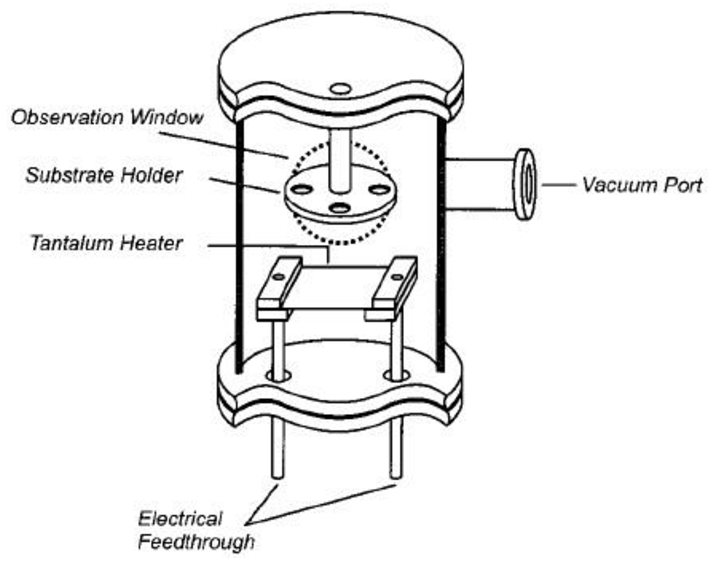
\includegraphics[width=0.7\textwidth]{Fig9}
%\caption{Cross section of single source thermal ablation apparatus. The starting material is placed on the tantalum heater, sublimates and forms a thin film on the substrate above. Reproduced from Ref.\ \cite{Chondroudis2000}.}
%\label{2Fig9}
%\end{figure}

\subsubsection{Spin coating}
Thin films can easily be produced by spin coating a perovskite solution on a substrate. Drops of solution are added to spinning substrates, and as the solvent evaporates a polycrystalline film is left behind. Suitable solvents include DMF \cite{Kikuchi2005}, THF \cite{Kataoka1994}, and acetonitrile \cite{VijayaPrakash2009}. The films produced have the same optical and electronic properties as single crystals, and the crystallographic $\vec{c}$ axis is perpendicular to the surface of the films \cite{Kataoka1993}. The films are generally smooth and can have a roughness of 1-2\,nm, although the solvent, substrate preparation, perovskite solution concentration, substrate temperature and spin speed all affect the thickness and morphology of films \cite{Mitzi2001b}. In thicker films, strain and uneven crystal planes lead to stacking imperfections, which may give rise to distorted quantum wells of differing widths and a decrease in the intensity of exciton absorption/luminescence \cite{VijayaPrakash2009}.

PbI perovskite samples tend to degrade over time due to moisture in the air, so a PMMA matrix doped with nanocrystalline PAPI can be created in order to suppress degradation \cite{Kitazawa1998}. PPMA, Pb$\textrm{I}_2$, and $\textrm{C}_6\textrm{H}_9\textrm{C}_2\textrm{H}_4\textrm{NH}_3\textrm{I}$ are dissolved in DMF then spin coated onto a glass substrate, and the resulting film annealed (thickness $\approx200$\,nm). The $\vec{c}$ axis of PAPI crystals are perpendicular to the surface of the film, and a strong exciton absorption at 2.4\,eV is seen as well as a step-like feature at 2.7\,eV due to interband transitions [Fig.\ \ref{2Fig10}(a)]. The binding energy of excitons in PMMA doped films is around 300\,meV, larger than in pure PAPI samples (250\,meV) due to dielectric confinement of PMMA. After two months in a humidity controlled box, absorption of the PAPI-doped PMMA sample is almost unchanged, however the spin coated PAPI film is degraded and no exciton peak can be seen [Fig.\,\ref{2Fig10}(b)].
\begin{figure}
\centering
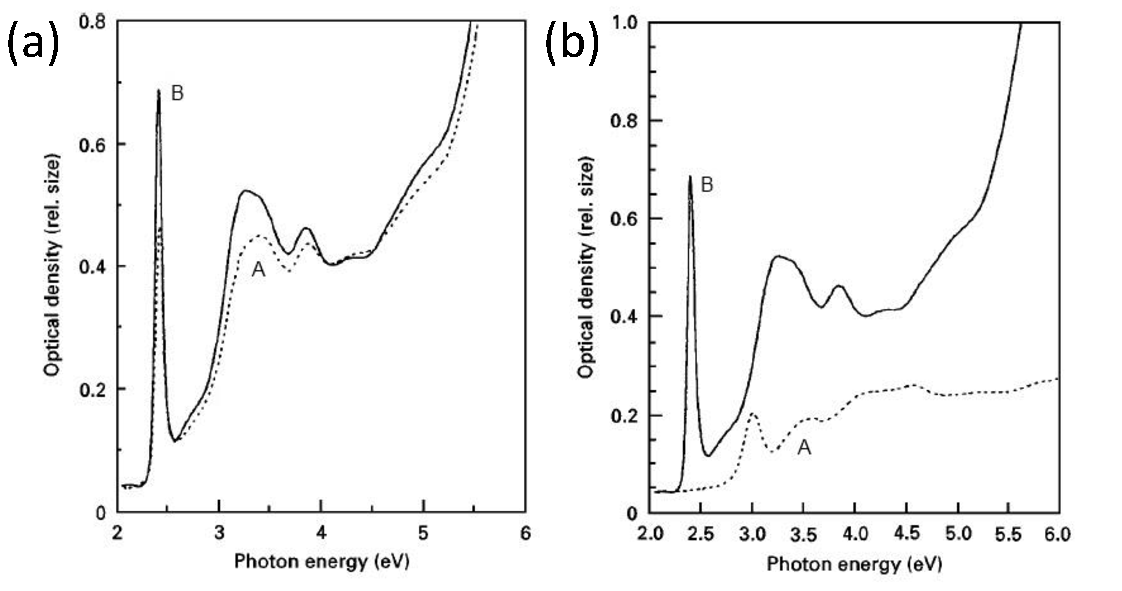
\includegraphics[width=\textwidth]{Fig10}
\caption{ (a) Absorption spectra of A) PAPI film spin coated using acetonitrile solution (dotted line), and B) PAPI doped PMMA annealed at $125^{\circ}$C for 10 minutes (solid line). (b) Absorption spectra of above films after being in a humidity controlled box for two months \cite{Kitazawa1998}.}
\label{2Fig10}
\end{figure}

The degradation of perovskite films is partly caused by the production of halide radicals, which can form halogen gases or react with organic moieties, Structures with more electron-rich organic molecules are therefore less resistant to attack from electrophilic halide radicals \cite{Wei2014}. Kondo \textit{et al.} reported oxygen($1s$) signatures in the photoelectron spectrum of photo-irradiated PAPI films, so photo-induced oxidation is another likely mechanism for photo-degradation \cite{Kitazawa2002}.

\subsubsection{Patterning}
Patterned PAPI films have been produced using a micromoulding in capillaries method (MIMIC). Polydimethylsiloxane (PDMS) moulds are created from silicon masters, then placed in conformal contact with pre-cleaned silicon substrates so the channels of the mould formed capillaries. A solution of PAPI dissolved in DMF is dropped on one end, and the channels are spontaneously filled by capillary force [Fig.\,\ref{2Fig11}(a)]. The mould and solution are then cured for 2\,hours at $65^{\circ}$C. In general the film stripes in Fig.\ \ref{2Fig11}(b) are defect free, however some edge defects are seen in C (channel width 0.8\,$\mu$m) since the channels are more difficult to fill when the width decreases. The width of film stripes also tend to be a little smaller than the width of mould channels, and a shrinkage of around 25\% is seen after solvent evaporation.  The patterned films have same the optical properties as unpatterened films \cite{Cheng2003}.
\begin{figure} [h!]
\centering
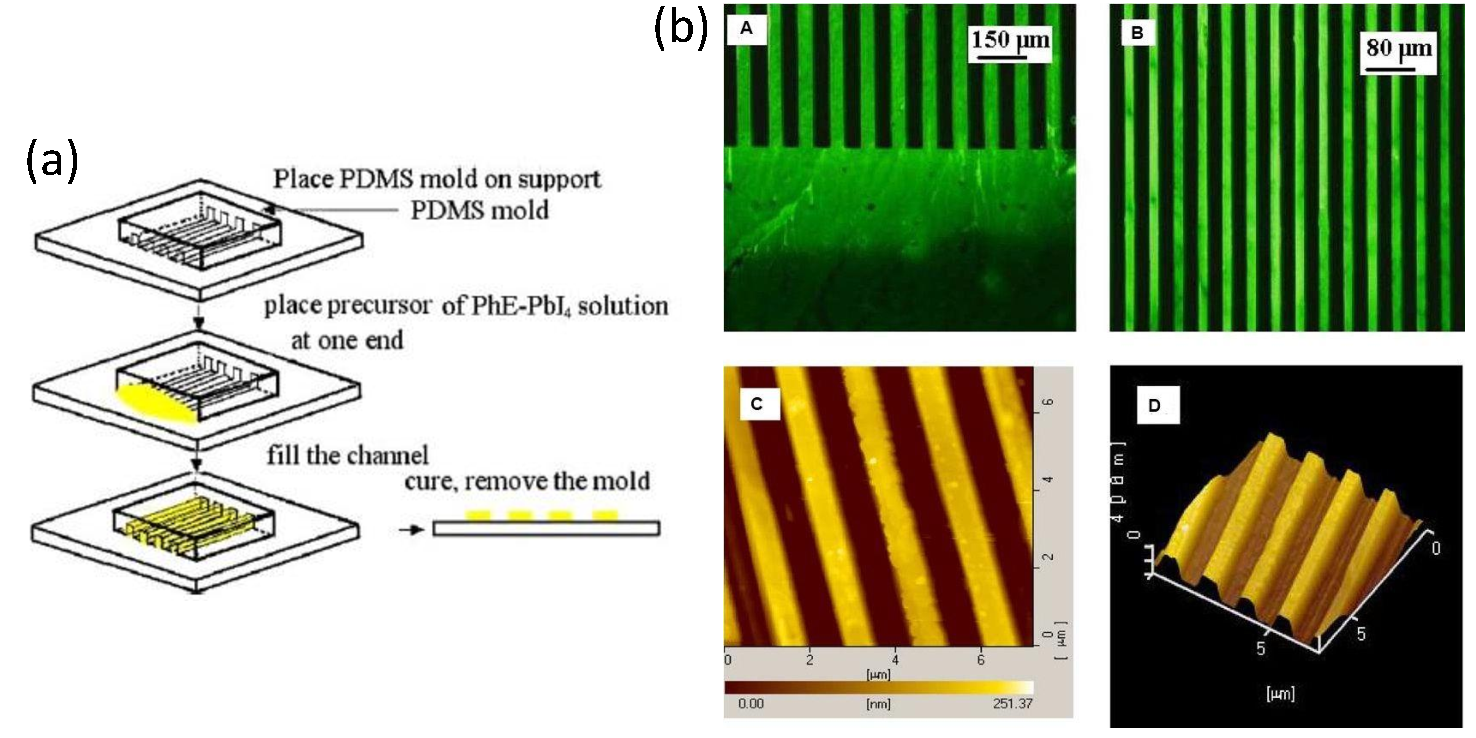
\includegraphics[width=\textwidth]{Fig11}
\caption{(a) Schematic of MIMIC process for pattering PAPI films. (b) Fluorescent optical micrographs (A,B) and AFM images (C: planar, D: stereo) of patterned PAPI films. In all cases the black stripes represent bare substrate without PAPI. Film stripe widths are A) 50\,$\mu$m wide, B) 15\,$\mu$m, C) and D) 0.8\,$\mu$m \cite{Cheng2003}.}
\label{2Fig11}
\end{figure}


\subsection{Electronic structure}
\begin{figure}[h!]
\centering
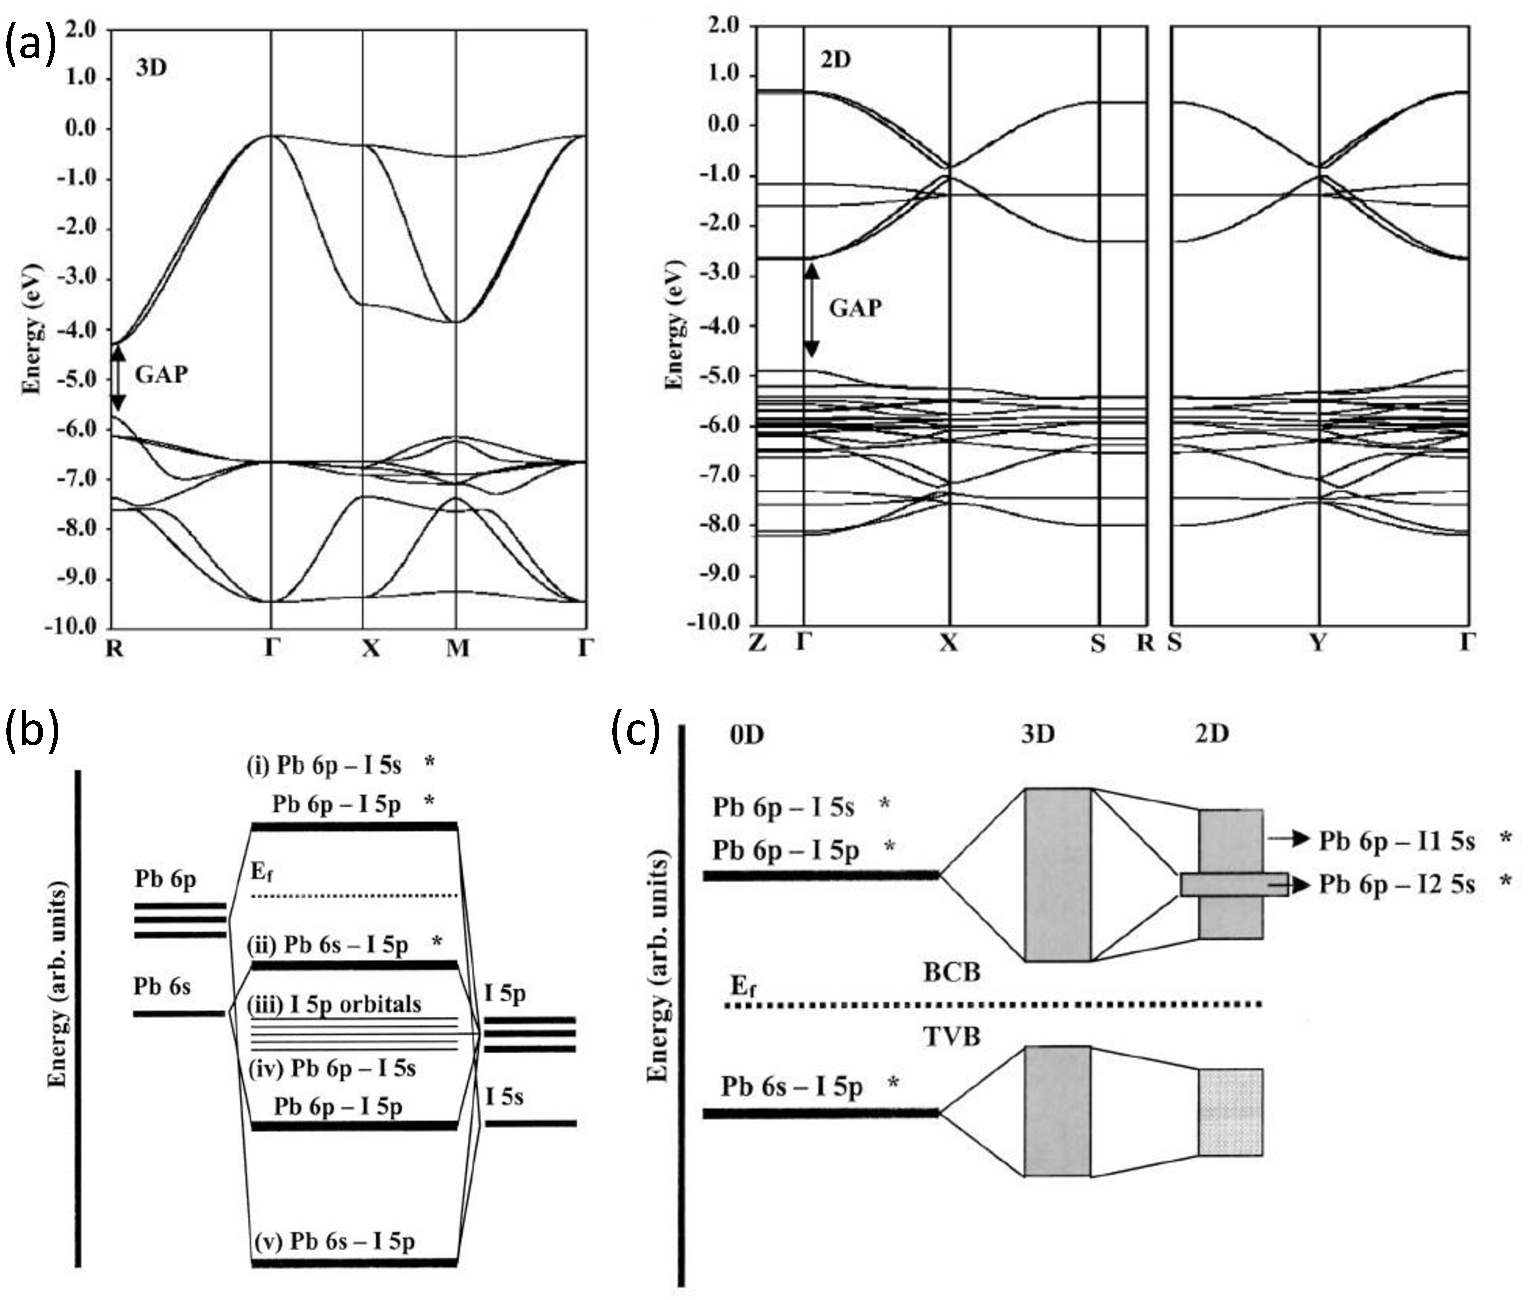
\includegraphics[width=\textwidth]{Fig12}
\caption{(a) Calculated band structures of $\textrm{CH}_3\textrm{NH}_3\textrm{PbI}_3$ (left) and $\textrm{C}_{4}$PI (right) along high symmetry lines in the first Brillouin zone. The band gap is labelled. Bonding diagrams of (b) one $\textrm{PbI}_6$ octahedron, and (c) extension to $\textrm{CH}_3\textrm{NH}_3\textrm{PbI}_3$ and $\textrm{C}_{4}$PI. The bottom of the conduction band (BCB), top of the valence band (TVB), and Fermi energy level ($\textrm{E}_F$) are labelled. Adapted from Ref.\ \cite{Umebayashi2003}.}
\label{2Fig12}
\end{figure}
Umebayashi \textit{et al.}\ calculated the electronic structure of $\textrm{C}_{4}$PI and its 3D extension $\textrm{CH}_3\textrm{NH}_3\textrm{PbI}_3$ using linear combination of atomic orbitals (LCAO) within density functional theory (DFT) [Fig.\,\ref{2Fig12}(a)] \cite{Umebayashi2003}. Both are direct gap semiconductors, but the 2D compound has a higher band gap and narrower bandwidths due to the decreased dimensionality. The 2D band structure also has flatter dispersions at the top of the valence band (TVB) and the bottom of the conduction band (BCB), leading to a larger carrier effective mass, and thus larger binding energy for excitons. 

Fig.\,\ref{2Fig12}(b) shows the bonding diagrams for a single $\textrm{PbI}_6$ octahedron, as well as the 3D and 2D compounds above. In the 2D crystal the TVB consists of Pb($6s$) and I($5p$) $\sigma$-antibonding orbitals, whereas the BCB consists of Pb($6p$) and I($5s$) $\sigma$-antibonding orbitals and Pb($6p$) and I($5p$) $\pi$-antibonding orbitals (not labelled on figure). The crystal field also lifts the degeneracy between different iodine atoms, so the conduction band with bridging iodine atoms ($\textrm{I}_1$) is wider than that with terminal iodine atoms ($\textrm{I}_2$). In Ref.\ \cite{Matsuishi2004} the BCB was labelled non-bonding from first principles pseudopotential total-energy calculations with the local density approximation, although it still consisted of Pb($6p$) and I($5p$) orbitals.

\subsection{Optical properties}
\subsubsection{Excitons}
\begin{figure}[h!]
\centering
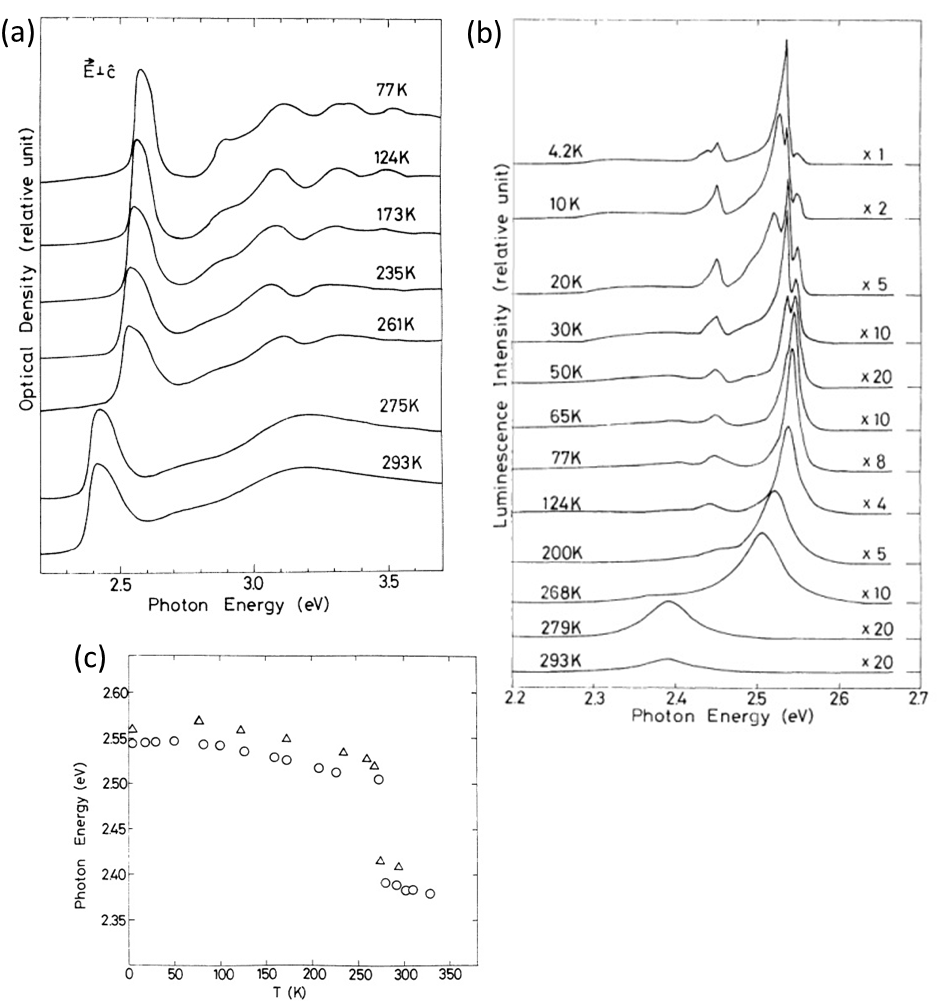
\includegraphics[width=\textwidth]{Fig13}
\caption{(a) Polarised optical density of $\textrm{C}_{10}$PI crystal at labelled temperatures, with $\vec{\mathbf{E}}$ parallel to the QWs. (b) Photoluminescence spectra spectra of $\textrm{C}_{10}$PI. The temperature and scaling of plotted data are labelled. (c) Energies of absorption ($\triangle$) and photoluminescence ($\circ$) peaks as a function of temperature \cite{Ishihara1990}.}
\label{2Fig13}
\end{figure}
Excitons are formed due to transitions between the TVB and BCB in the inorganic layers of PbI perovskites. Excitons in $\textrm{C}_{10}$PI have an energy of 2.4\,eV above 275\,K, but the value changes to 2.55\,eV at below 268\,K due to a phase transition of the alkylammonium molecules [Fig.\ \ref{2Fig13}]. The binding energy $E_B$ is calculated from the difference between the exciton peak and the step-like structure (interband transitions) in absorption spectra, and the value of $320\pm10$\,meV explains the presence of excitons at room temperature. Excitons also have a large oscillator strength of around $0.7\pm0.1$ \cite{Ishihara1990}. The above values are for the lowest energy ($n=1$) free exciton, but bound excitons can also be seen, for example in Fig.\,\ref{2Fig13}(b) the peak at 2.55\,eV is assigned to the lowest free exciton in the inorganic layers, whereas the peak at 2.53\,eV decreases in intensity with temperature and is assigned to a shallowly bound exciton. The peaks seen at low temperature $\sim2.45$\,eV are sample dependent, and thus assigned to deeply impurity-bound excitons \cite{Ishihara1990}. The Stokes shift for $\textrm{C}_{10}$PI is less than 5\,meV [Fig.\,\ref{2Fig13}(c)], and this is generally true for PbI-based perovskites (e.g. for $\textrm{C}_{12}$PI in Ref.\,\cite{Pradeesh2009}). In Refs.\,\cite{Ishihara1990, Ishihara1989} both longitudinal and transverse exciton-polaritons are observed in reflection spectra of $\textrm{C}_{10}$PI at 1.6\,K, with a splitting of around 60\,meV \cite{Ishihara1990}. The exciton radiative lifetime is 7\,ps at 8\,K \cite{Kondo1998a}.

Polarisation-dependent excitons are seen in the Kramers-Kronig calculated absorption spectra of diammonium \ce{(H3NC6H13NH3)PbI} [Fig.\,\ref{2Fig14}]. When the incoming light is polarised parallel to the crystallographic $\vec{b}$ axis, the lowest exciton has an energy of 2.5272\,eV. Two shoulders seen at 2.566 and 2.718\,eV (indicated by small arrows) are due to vibronic bands. The very small peak at 2.819\,eV is attributed to $n=2$ excitons, as determined using exciton activation energies calculated from PL spectra. Due to the monoclinic crystal symmetry, light polarised parallel to $\vec{c}$ can generate excitons polarised along both the $\vec{a}$ and $\vec{c}$ axes. And as the $\vec{a}$ and $\vec{b}$ directions are very nearly isotropic, the peak at 2.5272\,eV (also seen in Fig.\,\ref{2Fig14}(a)), is attributed to excitons polarised parallel to $\vec{a}$. The narrow peak at 2.559\,eV is due to excitons polarised parallel to $\vec{c}$, but only appears at very low temperatures as the linewidth normally causes the two exciton peaks to be indistinguishable. The binding energy for the material is calculated to be 330\,meV, and the Bohr radius 8.2\,\AA \cite{Goto2001}.
\begin{figure} [h!]
\centering
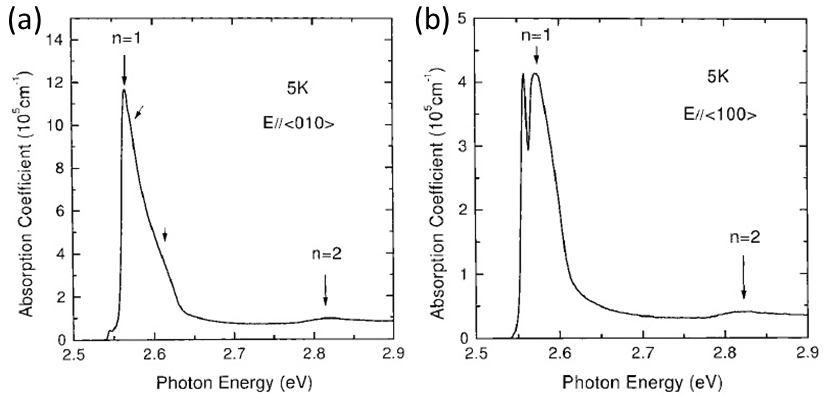
\includegraphics[width=\textwidth]{Fig14}
\caption{Absorbance spectra for $\vec{\mathbf{E}}$ parallel to (a) $\vec{b}$, and (b) $\vec{c}$ axes for \ce{(H3NC6H13NH3)PbI4}, calculated using Kramers-Kronig relations from reflection spectra. The $n=1, 2$ peaks are labelled, and arrows indicate vibronic sidebands \cite{Goto2001}.}
\label{2Fig14}
\end{figure}

The band gap of perovskites can be engineered by altering the halogen and metal atoms in the structure. The exciton energy ranges from 2.5\,eV for PbI perovskites, to 3.1\,eV for PbBr and 3.6\,eV for PbCl. Indeed mixed-halide perovskites of the form \ce{(RNH3)2Pb}$\textnormal{A}_x\textnormal{B}_{1-x}$ allow variation within this range \cite{Kitazawa1996, Kitazawa1997}. It has been shown that the while the change in absorption wavelength generally varies linearly with the halogen concentration $x$, because the process is averaged over excitons at all possible sites, the excitons formed then preferentially diffuse over $\sim10$\,nm to lower energy halogen atomic sites so the emission wavelength does not show the same linear variation with $x$ \cite{Ahmad2013}.

There has been some discussion regarding the nature of the excitons. Xu \textit{et al.} used magneto-optical measurements on polycrystalline $\textrm{C}_{10}$PI thin films and found that exciton peaks are not shifted when a magnetic field is applied in the plane of the QWs. However when the field is perpendicular to the QWs the energy of the exciton $E$ changes according to
\begin{equation}
E = E_0 \pm \frac{1}{2} g_{\bot} \mu_{B} B + c_0 B^2~,
\label{mag-shift}
\end{equation} 
where $E_0$ is the energy of the exciton at zero field, $g_{\bot}$ is the Land\'{e} $g$ factor perpendicular to the plane of the film, $\mu_B$ is the Bohr magneton, and $c_0$ is the diamagnetic constant. The sign of the energy shift depends on the polarisation of the magnetic field, and from the data $g_{\bot}\sim1$, and $c_0\sim 10^{-7}$~eV/$\textrm{T}^2$ for C$_{10}$PI. From the magneto-absorption measurements $a_B \sim12\,$\AA for $\textrm{C}_{10}$PI. The peak shifts indicate $\textrm{C}_{10}$PI excitons are Wannier-like, since Frenkel excitons would have no extended motion and thus show no energy shift at all. However as the size of each $\textrm{PbI}_6$ octahedron is around 6\,\AA~\cite{Ishihara1990}, excitonic motion extends over only a few octahedra \cite{Xu1991b}.

Magneto-optical measurements on C$_6$PI produces $g_{\bot}$ and $c_0$ values similar to those in $\textrm{C}_{10}$PI, however the authors believed that as the exciton Bohr radius is on the order of Pb-Pb distances in the crystal, the exciton may be better described by a cationic Frenkel model involving orbitals of Pb$^{2+}$. The calculated $g_{\bot}$ and $c_0$ agree well with experiment \cite{Kataoka1993}. On the other hand Tanaka \textit{et al.}\ used electroabsorption and two-photon absorption studies and showed that excitons in thin film $\textrm{C}_{6}$PI samples were Wannier-like in nature, with 1s, 2s, 2p, and 3p energies at 2.34, 2.60, 2.61, and 2.64\,eV respectively. The Wannier excitons exhibited strong 2D behaviour, and for the 1s exciton $E_B = 310$\,meV \cite{Tanaka2002}.


\subsubsection{Biexcitons and triexcitons}
\begin{figure}[h!]
\centering
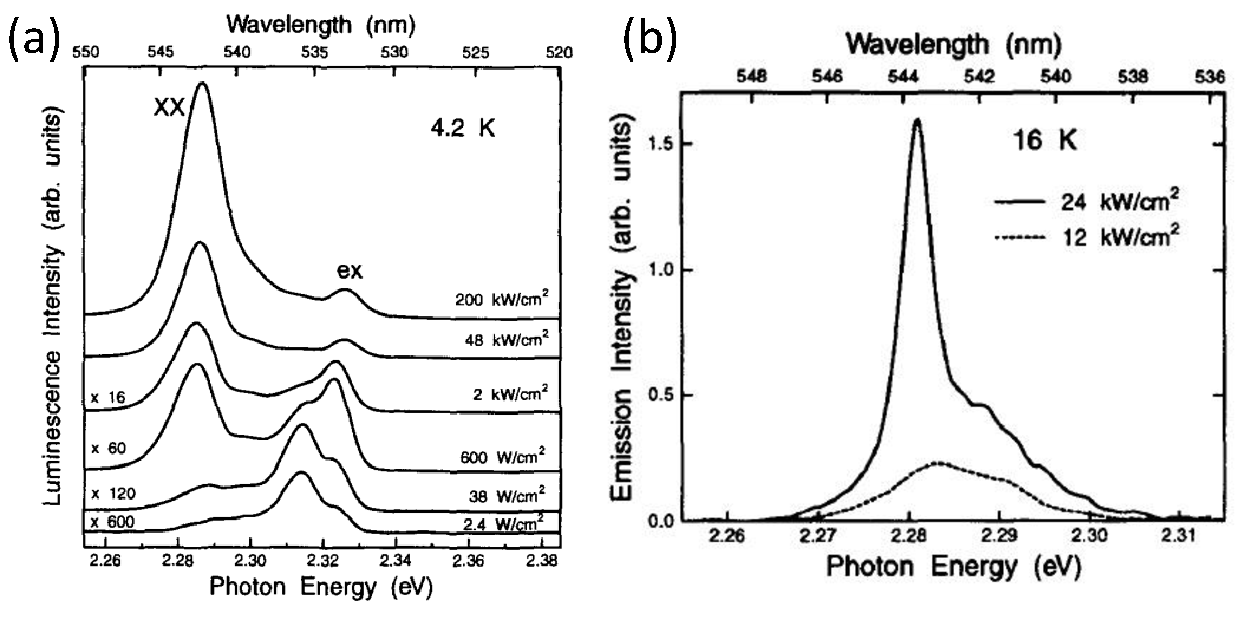
\includegraphics[width=\textwidth]{Fig15}
\caption{(a) Photoluminescence spectra of $\textrm{C}_{6}$PI film excited by 337\,nm nitrogen laser at 4.2\,K. The excitation intensity and data scaling are given. Exciton (ex) and biexciton (XX) bands are labelled. (b) Emission spectra of $\textrm{C}_{6}$PI waveguide above (24\,kW/$\textrm{cm}^2$) and below (12\,kW/$\textrm{cm}^2$) the lasing threshold at 4.2\,K. The lasing wavelength is 543.6\,nm \cite{Kondo1998}.}
\label{2Fig15}
\end{figure}
An increase in excitation power can lead to the formation of bi- or tri-exciton complexes, where two or three free excitons are bound together. Induced photo-carriers screen Coulomb interactions, so strong interactions between carriers are needed to observe triexcitons. Low dimensionality is an advantage as screening has a more limited effect \cite{Shimizu2006a}. The radiative decay of biexcitons to transverse excitons has been observed in \ce{C6PI} [Fig.\,\ref{2Fig15}(a)] and $\textrm{C}_{10}$PI, with biexciton binding energy of $\sim50$\,meV \cite{Kondo1998, Ishihara1992}. By creating a waveguide configuration with transverse pumping, biexciton lasing is observed in $\textrm{C}_6$PI. The lasing threshold is 20\,kW/$\textrm{cm}^2$ at 16\,K. Fig.\ref{2Fig15}(b) shows emission spectra above and below the lasing threshold: a broad biexciton band is seen below the threshold, but a sharp peak at 2.281V can be observed above the threshold. The biexciton band is probably isotropic as the emission is not polarised \cite{Kondo1998}.

\begin{figure}[h!]
\centering
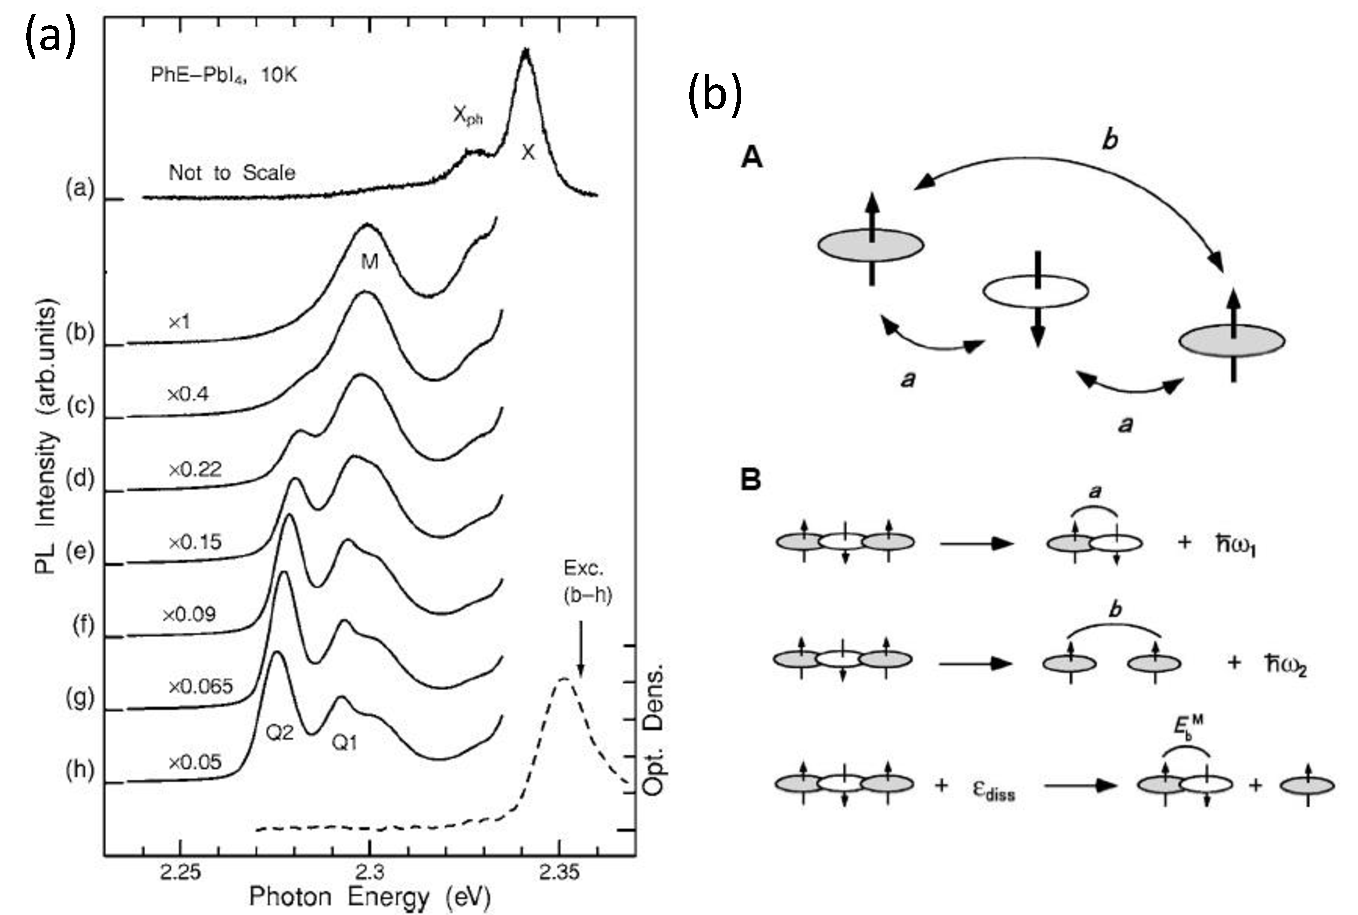
\includegraphics[width=\textwidth]{Fig16}
\caption{(a) PL spectra of PAPI at different excitation intensities and energies. (a) is excited at 2.58eV, and (b)-(h) at 2.355eV. The excitation intensities are (a) $4.6\times 10^{10}$, (b) $4.6\times 10^{12}$, (c) $1.4\times 10^{13}$, (d) $2.8\times 10^{13}$, (e) $4.6\times 10^{13}$, (f) $9.2\times 10^{13}$, (g) $1.6\times 10^{14}$, and (h) $3.2\times 10^{14}$ photons c$\textrm{m}^{-2}$. The dotted line shows the absorption spectrum. X is the free exciton band, $\textrm{X}_{\textrm{\footnotesize ph}}$ phonon sidebands, M the biexciton band, $\textrm{Q}_1$ amplified spontaneous recombination of biexcitons, and $\textrm{Q}_2$ the $\hbar \omega_2$ triexciton process. (b) A) shows the triexciton model, and B) likely dissociation mechanisms. For the meaning of symbols see the main text \cite{Shimizu2006a}.}
\label{2Fig16}
\end{figure}

Shimizu \textit{et al.}\ observed triexciton formation in the PL spectra of PAPI. In Fig.\ \ref{2Fig16}(a), the free exciton band is labelled X, phonon sidebands $\textrm{X}_{\textrm{\footnotesize ph}}$, and the biexciton band M. At higher excitation intensities, two other bands can be seen, labelled $\textrm{Q}_1$ and $\textrm{Q}_2$. $\textrm{Q}_1$ is assigned to the amplified spontaneous emission due biexciton recombination, and $\textrm{Q}_2$ to a triexciton process. Triexcitons consist of bound states of three spin singlet excitons, with interaction energy $a$ between opposite spin excitons ($<0$), and interaction energy $b$ between same spin excitons ($>0$). Likely radiative triexciton dissociation mechanisms are dissociation into a biexciton and photon $\omega_1$, or two excitons and photon $\omega_2$. However nonradiative dissociation (energy $\epsilon_{\textrm{\footnotesize diss}}$) into a biexciton (binding energy $E_{\textrm{\footnotesize b}}^{\textrm{\footnotesize M}}$) and an exciton is also possible [Fig.\,\ref{2Fig16}(b)]. As $\textrm{Q}_2$ is at a lower energy than M, it can only be due to the $\omega_2$ process, although it is unclear why the $\omega_1$ process is not observed. From the data collected, $a=-37.5$\,meV, $b=11$\,meV, $\epsilon_{\textrm{\footnotesize diss}}=14$\,meV, and $E_{\textrm{\footnotesize b}}^{\textrm{\footnotesize M}}=50$\,meV \cite{Shimizu2006a}. 


\subsubsection{Dielectric confinement and the image charge effect}

Both the binding energy and oscillator strength of (transverse) excitons in 2D PbI perovskites are much larger than those in the inorganic 3D equivalent Pb$\textrm{I}_2$ \cite{Hirasawa1994}. In materials where a QW is sandwiched between barrier layers with lower dielectric constant $\epsilon_b$, three types of confinement affect excitons. Firstly quantum confinement, where the reduction in dimensionality to 2D gives a binding energy four times larger than expected in bulk 3D material for the $n=1$ exciton as discussed in Section \ref{sec:ex2D} \cite{Shinada1966}. Secondly dielectric confinement, where the lower barrier $\epsilon_b$ reduces the effective dielectric constant of the entire structure, thus providing less shielding and giving a higher binding energy. Thirdly mass confinement, where carrier wavefunctions extending into the barrier region lead to a larger effective mass, thus increasing the binding energy. Mass confinement depends on quantum confinement in order to determine how much of the carrier wavefunction is leaked into the barrier region, and generally only has a small effect \cite{Kumagai1989}. The interfaces between layers also act as mirrors which create an infinite series of image charges [Fig.\ \ref{2Fig17}]. Using carrier wavefunctions which fit the boundary conditions of the well, as well as self and image-charge Hamiltonians, exciton properties can be calculated. The results show that $E_B$ increases if the barrier height decreases, the excitons have larger effective mass in carrier region, or the barrier regions have a smaller dielectric constant \cite{Kumagai1989}. Muljarov \textit{et al.}\ found that the potentials created due to the image charge effect causes charges in the inorganic layers to be repelled from the interface, whereas charges in the organic layers are attracted to the interface \cite{Muljarov1995}.
\begin{figure}[h!]
\centering
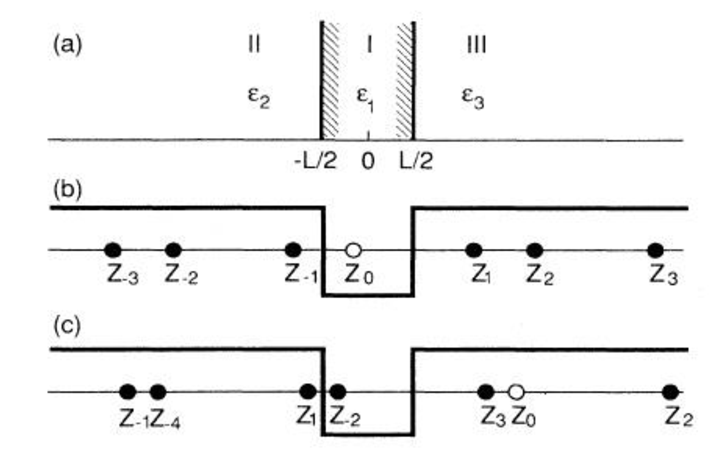
\includegraphics[width=0.8\textwidth]{Fig17}
\caption{(a) Generalised description of quantum well (region I) and barriers (regions II and III). (b) and (c) show the positions of initial charges (white circle, $Z_0$) and image charges created (black circles) due to interfaces. In (b) the initial charge is in the well region, whereas in (c) it is in the barrier region \cite{Kumagai1989}.}
\label{2Fig17}
\end{figure}

\subsection{Organic molecules}
The way organic molecules fit into the perovskite structure can change the conformation of \ce{PbI6} octahedra, the Pb-I bond angle or the interlayer I-I coupling, all of which lead to a change in the electronic structure \cite{Sourisseau2007}. Pb-I-Pb bond angles have the greatest effect on the band gap of perovskites. Experimental results show that bond angles closer to $180^{\circ}$ (undistorted octahedra) lead to smaller $E_g$, which agrees with extended Huckel tight-binding calculations used to evaluate band structures of PbI perovskites [Fig.\ \ref{2Fig19}]. Although $E_g$ is underestimated using this model, the overall correlation between I-Pb-I angle and electronic energy levels are correct \cite{Pradeesh2009}. Calculations for Sn-based perovskites show that bond angle distortions in the QW plane have a larger impact on $E_g$ than purely out-of-plane distortions \cite{Knutson2005}. For this reason, pressure can be used as an external parameter to tune to exciton energy \cite{Matsuishi2001}.
\begin{figure}[h!]
\centering
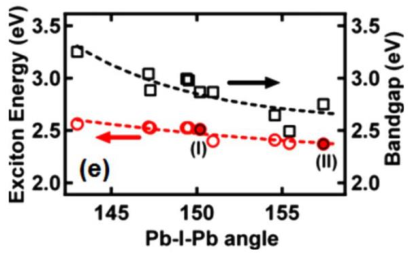
\includegraphics[width=0.6\textwidth]{Fig19}
\caption{Variations in exciton energy (red) and band gap (black) with Pb-I-Pb angles calculated using extended Huckel tight binding calculations. Data points given are experimentally determined for PbI perovskites, and filled in circles represent PL maxima of labelled $\textrm{C}_{12}$PI phases \cite{Pradeesh2009}.}
\label{2Fig19}
\end{figure}

2,$2^{'}$-biimidazole ($\textrm{C}_6\textrm{H}_6\textrm{N}_4$) can be incorporated into the perovskite structure to form $(\textrm{C}_6\textrm{H}_8\textrm{N}_4)\textrm{PbI}_4$. The loss of \ce{NH3} groups, as well as the ability to delocalise charge across the organic molecule, leads to weaker hydrogen bonding with inorganic octahedra. Thus the reduced corrugation of QWs produces smaller $E_g$ compared to C$_n$PI \cite{Tang2001}. Similarly in $(\textrm{HO(CH}_2)_2\textrm{NH}_3)_2\textrm{PbI}_4$, the OH group is able to hydrogen bond with neighbouring $\textrm{NH}_3$ groups or I atoms. The extra interactions weaken the $\textrm{NH}_3$-I hydrogen bonds, and also provide a channel for stronger electronic coupling between inorganic layers, leading to smaller $E_g$ \cite{Mercier2004}.

In general perovskites have better PL efficiencies if the QWs are flat. Therefore as well as bonding with functional groups of the organic molecule, the most emissive compounds are created using relatively flexible molecules whose size allows the formation of the MQW structure without too much deformation of inorganic sheets \cite{Zhang2009}.

As well as structural effects, notable properties of the organic ligand can be be incorporated into the perovskite. For example perovskites with with chiral molecules also exhibit optical activity \cite{Teshima2003}, while inclusion of chromophores into the structure can lead to charge and energy transfer between the organic and inorganic layers \cite{Kawabata2009, Mitzi1999a, Braun1999}.

\subsection{Applications}
\subsubsection{Microcavities and photonic crystals}
The dynamics of interactions between quasiparticles can be described in two limiting regimes. In the weak coupling limit the system can still be described by the original quasiparticle wavefunctions, albeit with some perturbations. In the strong coupling limit, coherent interactions between quasiparticles lead to the formation of mixed states that oscillate between the original eigenstates with frequency $\Omega_R$ (Rabi frequency, also a measure of the interaction strength). The new mixed states can combine properties of both the original particles. For example, strong coupling between excitons and cavity photon modes create exciton-polaritons, quasiparticles with small effective mass but capable of nonlinear interactions, polaritons have shown great promise in producing Bose-Einstein condensates \cite{Kasprzak2006}, low-threshold lasers \cite{Christopoulos2007} and ultrafast switches \cite{Amo2010}.
\begin{figure}[h!]
\centering
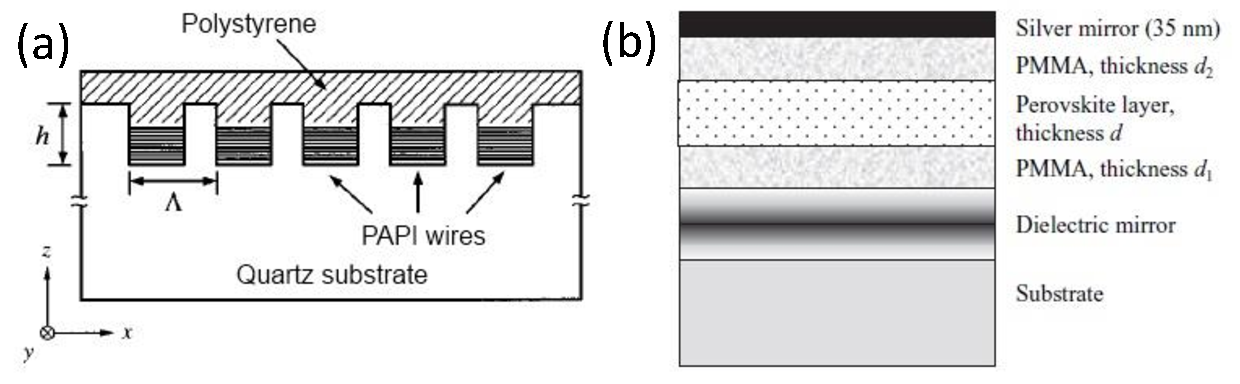
\includegraphics[width=\textwidth]{Fig20}
\caption{(a) Schematic of a distributed feedback microcavity. (b) Transmission dip positions at normal incidence as a function of cavity detuning from the PAPI exciton energy. Closed circles and diamonds represent the upper and lower polariton branches respectively, while closed squares indicate upper branch polaritons not affected by the reciprocal lattice vectors \cite{Fujita1998}.}
\label{2Fig20}
\end{figure}

Strong coupling has been observed between PAPI excitons and cavity modes in a distributed feedback microcavity at room temperature \cite{Fujita1998, Fujita1999, Fujita2000}. The cavity consists of a structured quartz substrate with PAPI spin coated into the spaces to form parallel wires, and an overcoat of polystyrene added to prevent the degradation of PAPI films [Fig.\,\ref{2Fig20}(a)]. When the incident beam is at normal incidence, PAPI excitons and fourth order cavity resonance become resonant, couple strongly and form new eigenstates (cavity polaritons). Using a variety of grating pitches $\Gamma$ from 0.62 to 0.72\,$\mu$m, transmission spectra showed that the upper and lower polariton branches exhibit anticrossing behaviour, as expected for strongly coupled modes [Fig.\,\ref{2Fig20}(b)]. Due to the large exciton oscillator strength, the mode splitting is around 100\,meV, an order of magnitude larger than the 9\,meV observed in GaAs systems in Fabry-Perot microcavities \cite{Fujita1998}. A strong enhancement of PL intensity of the lower branch polariton is seen if the standing wave cavity mode is in resonance with PAPI excitons, in this case when $\Gamma=0.68\,\mu$m \cite{Fujita1999}. No signature of the upper polariton branch is seen as in thermodynamic equilibrium the upper branch would expect to be less populated, however the polariton lifetime may not be long enough for equilibrium to occur. Other suggestions have included a relaxation of the upper branch polaritons towards uncoupled excitonic states, or fast emission of photons between the upper and lower polariton branches \cite{Lanty2008}. It is thought that PAPI rods oscillating in phase due to strong coupling with cavity modes at resonance would lead to a macroscopic polarisation and ultrafast resonance, however the polariton lifetime is actually 8\,ps longer with a grating structure at 40\,K. It is possible that this is due to excitons with large wave vectors that cannot couple to the outside without the help of the grating reciprocal lattice vector \cite{Fujita2000}. Strong coupling between excitons and 2D grating modes has also been observed in PAPI with Rabi splitting 100\,meV \cite{Ishi-Hayase2003}.

Strong coupling between cavity and PAPI exciton modes are also observed in the Fabry-Perot microcavities \cite{Brehier2006, Lanty2008}. By adjusting the position of the perovskite layer in the microcavity, the coupling between exciton and photon modes can be controlled, and the splittings seen were between 130-190\,nm. Similar CHPI microcavities constructed produce splittings of 130\,meV for a $5\lambda/4$ metal-air microcavity, and of 160\,meV for a $7\lambda/4$ metal-metal microcavity \cite{Pradeesh2009b}.

Strong exciton-photon coupling has also been observed in a photonic crystal of 256\,nm diameter microspheres infiltrated with PAPI (silica opal) \cite{Sumioka2001}. A face centred cubic lattice of silica microspheres with 3D channel voids is created, and a solution of PAPI and DMF introduced into continuous spaces through capillary forces [Fig.\,\ref{2Fig21}(a)]. Angle-dependent reflectivity spectra of the structure with PAPI filling fraction $f_{\textnormal{PAPI}}=0.06$ clearly demonstrates anticrossing behaviour, indicating strong coupling between the stop band (photon mode) of the photonic crystal and the exciton mode of PAPI, with Rabi splitting 240\,meV [Fig.\,\ref{2Fig21}(b)]. However there is an uncoupled exciton mode that seems largely unaffected by the photon mode, possibly due to some of the bulk PAPI on the surface of the silica opal remaining, or an open photonic gap in the silica opal that leads to insufficient photon confinement and limits exciton-photon coupling. 
\begin{figure}[h!]
\centering
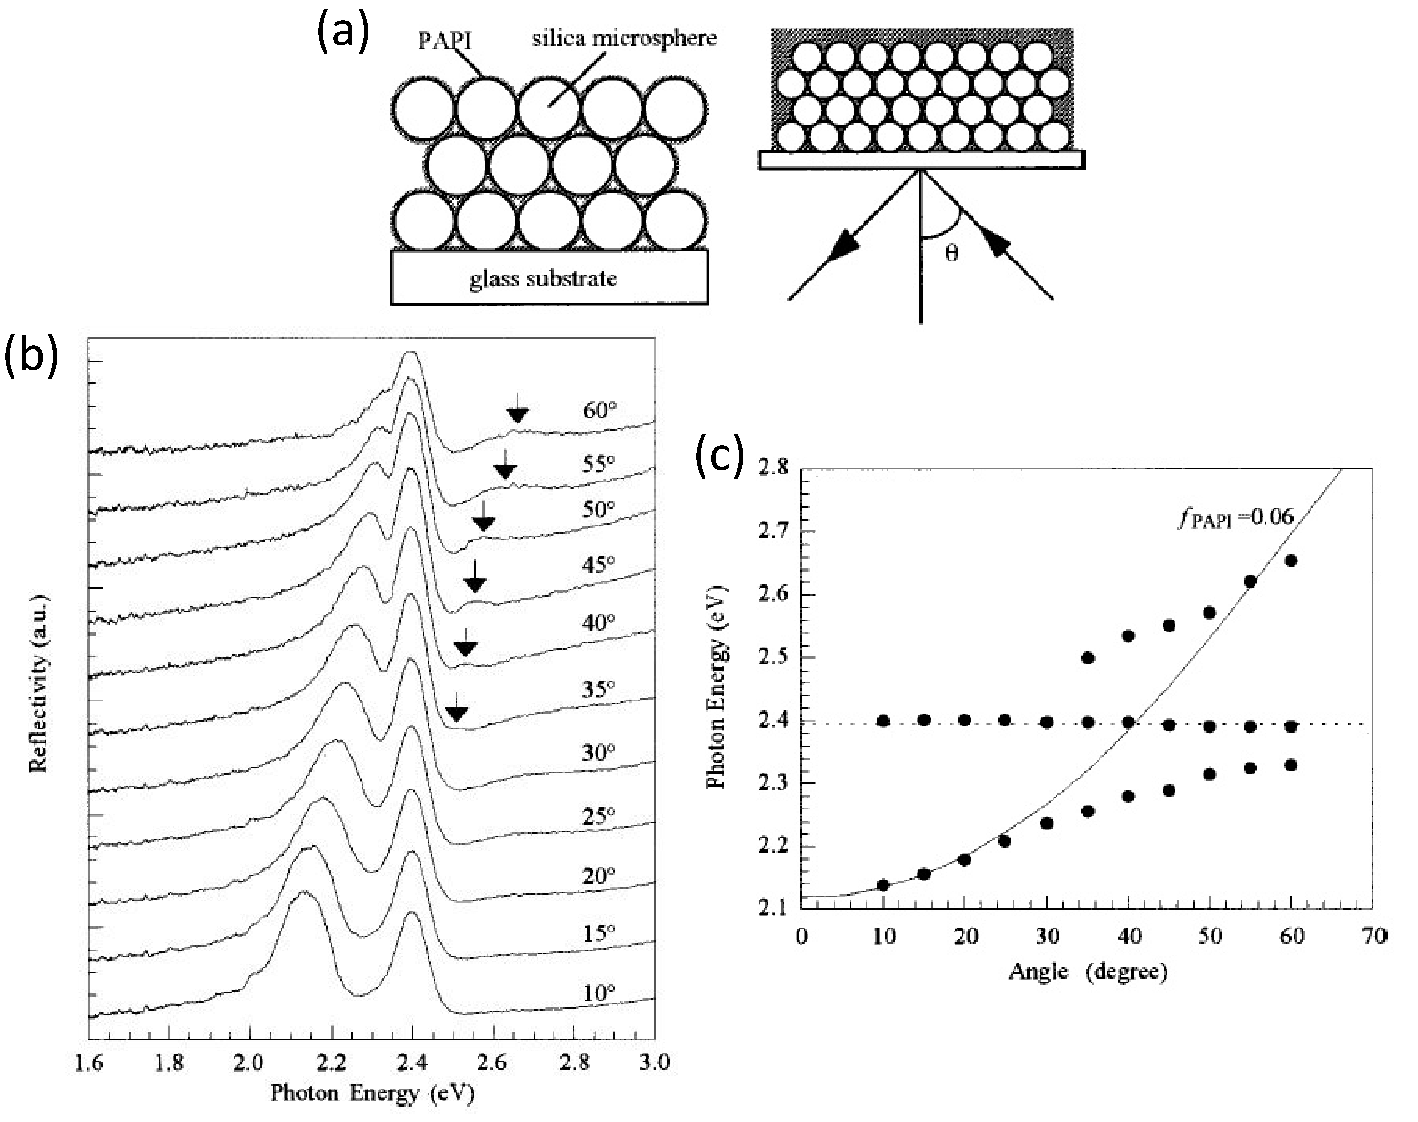
\includegraphics[width=\textwidth]{Fig21}
\caption{(a) Structure of silica opal infiltrated with PAPI film formed on a glass substrate. (b) Extracted mode positions from angle-dependent reflectivity spectra (black circles) for opal with PAPI filling fraction $f_{\textnormal{PAPI}}=0.06$. Exciton energy (dashed line) and theoretical photonic crystal stop gap (solid line) are marked \cite{Sumioka2001}.}
\label{2Fig21}
\end{figure}

\subsubsection{Optoelectronic devices}
The processability of perovskites from solution and their high PL efficiencies make perovskites attractive for optoelectronic devices, particularly electroluminescent (EL) devices. Era \textit{et al.}\ used a layered structure consisting of PAPI, an indium-tin-oxide (ITO) anode, MgAg cathode, and oxadiazole (OXD7) electron transport layer [Fig.\,\ref{2Fig22}(a)]. When the device is driven, electrons in OXD7 are injected smoothly into the PAPI layer as there is no energy barrier, but holes injected into PAPI will remain at the PAPI/OXD7 interface due to the barrier potential [Fig.\,\ref{2Fig22}(b)]. Electrons and holes are therefore trapped in the PAPI layer, and recombine to provide luminescence. When driven at liquid nitrogen temperatures, the EL intensity reaches a luminescence of more than 10000\,cd$\textrm{m}^2$ at a current density of 2\,A$\textrm{cm}^{-2}$ and voltage of 24\,V. The emission peak at 520\,nm has narrow bandwidth, and is very similar to the PL spectrum. However the EL efficiency at room temperature is much smaller than that at liquid nitrogen temperatures, and is mainly caused by thermal ionisation of excitons \cite{Era1994}. Similar devices made by Matsushima \textit{et al.} [Fig.\,\ref{2Fig22}(c)] show that an additional buffer layer (OTS=octadecyltrichlorosilane, CuPc=Cu pthalocyanine) can reduce the hole-injection barrier between ITO and PAPI, leading to an increase in EL efficiency. Buffer layers that decrease PAPI film roughness will also reduce leakage current \cite{Matsushima2005}.
\begin{figure}[h!]
\centering
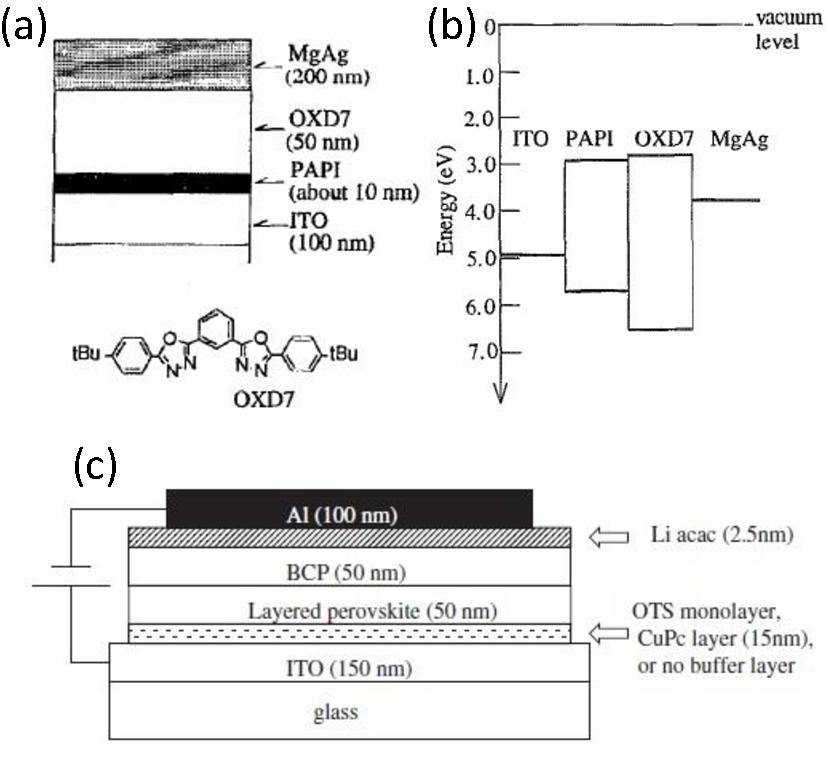
\includegraphics[width=0.8\textwidth]{Fig22}
\caption{(a) Schematic of EL device with PAPI by Era \textit{et al.}, and (b) energy level diagram of the device \cite{Era1994}. (c) Schematic of the LED made using PAPI by Matsushima \textit{et al.} \cite{Matsushima2005}.}
\label{2Fig22}
\end{figure}

Hattori \textit{et al.}\ made EL devices shown in Fig.\,\ref{2Fig22}(a) using PBPI (\ce{(C6H5C4H8NH3)2PbI4}), PAPI and CHPI. As before the EL and PL of all three compounds are almost identical [Fig.\,\ref{2Fig23}(a)], however despite PBPI and CHPI having higher PL efficiencies than PAPI [Fig.\,\ref{2Fig23}(b)], the PBPI device had the lowest external quantum efficiency $\eta_{ext}$ (number of emitted photons/number of electrons) and CHPI the highest. The PBPI device is also much more resistive than the others, with current density around two orders of magnitude less than other devices at same voltage. Both the resistance and the low EL efficiency are likely due to the longer alkyl chain preventing carrier transport. The external efficiency of the CHPI device is comparable to the highest efficiency reported in EL devices reported at the time \cite{Hattori1996}.
\begin{figure}[h!]
\centering
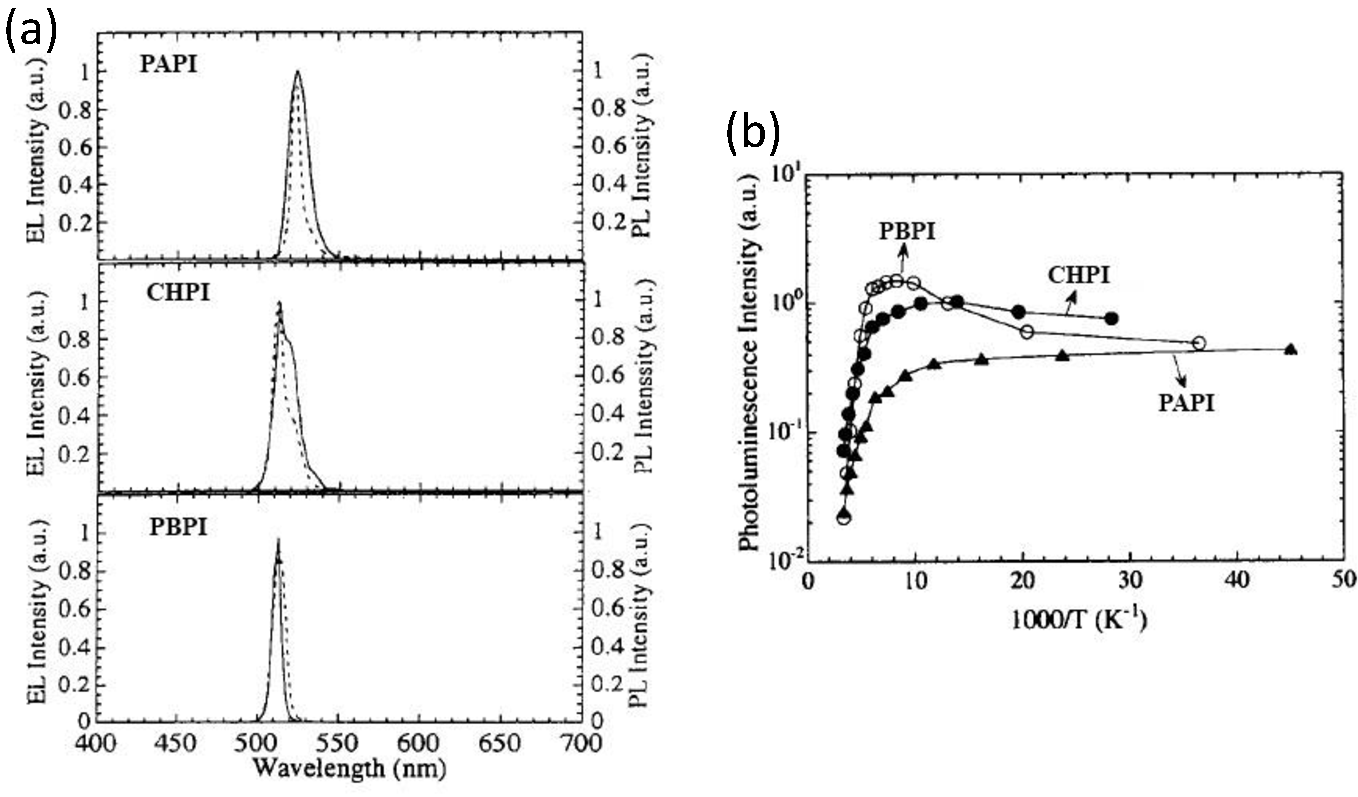
\includegraphics[width=0.6\textwidth]{Fig23}
\caption{(a) EL (solid lines) and PL (dotted lines) spectra of the labelled perovskite at 110\,K. EL device structure is shown in Fig.\ \ref{2Fig22}(a). (b) Integrated PL intensity of CHPI, PAPI, and PBPI thin film samples as a function of temperature \cite{Hattori1996}.}
\label{2Fig23}
\end{figure}

Although there have not been many studies on the transport properties of 2D PbI perovskites, SnI perovskites have received more attention in this area. 2D SnI structures are semiconducting, while the 3D SnI perovskite is a low-carrier density p-type metal \cite{Mitzi1994}. Thin film transistors have also been produced from 2D SnI perovskites, with carrier mobilities of up to 1.4\,cm$^2$/Vs, better than that of amorphous silicon, with on-off ratio $>1000$ and current densities $>400$\,A/cm$^2$ \cite{Mitzi2002b, Mitzi2001d, Kagan1999a}.

\subsubsection{Scintillators}
Scintillators convert radiation energy into photo-emission for the purpose of detecting ionising radiation. They need to have a short luminescence decay time constant in order to react quickly, high resistance to radiation damage, and high efficiency so that a suitable number of photons are created per unit radiation energy of absorbed \cite{Shibuya2002}. Many efficient scintillators (e.g.\ NaI:TI, CsI:Na) have decay times of 200\,ns or more, whereas fast scintillators (e.g.\ Ba$\textrm{F}_2$, CsF) have low light yields of less than 2000~photons per MeV \cite{Kengo2002}. $\textrm{C}_6$PI crystals are bombarded by an ultra-short electron beam with pulse width of 1-2\,ps, generated by a 35MeV linear accelerator, and produced a decay constant of 45\,ps at room temperature \cite{Kengo2002}. Investigations show 2D perovskites have faster decay times than their 3D counterparts as quantum confinement provides carrier wavefunction overlap and higher likelihood of decay.

Shibuya \textit{et al.}\ used different dosages of 2\,MeV protons to test $\approx250$nm thick $\textrm{C}_6$PI thin films \cite{Shibuya2002}. Radiation-induced emission spectra show no shift in the exciton peak position during bombardment, and no additional peaks appeared at any radiation dosage. Three decay components are found: one with decay constant 0.39\,ns due to free exciton recombination, then two defect density dependent components with constants of 3.8 and 16\,ns due to trapped excitons, with decay constants depending on defect density. Emission intensities of $\textrm{C}_6$PI excitons attenuated with increased radiation, but the radiation hardness is still enough for practical use. From these results, $\textrm{C}_6$PI is a good candidate for scintillator use due to the stability of excitons at room temperature, ease of processing, fast response time, spectrum stability to radiation, and inclusion of high atomic number element (Pb) in order to detect low energy transfer radiation such as X-rays \cite{Shibuya2004}. 

\section{Conclusions}
Excitons, bound hydrogen atom-like systems of electrons and holes, produce strong optical signatures in semiconductors, and many exciton effects are enhanced by a reduction in dimensionality. 2D hybrid organic-inorganic perovskites are naturally self-assembling materials that create a MQW structure, whose room temperature optical properties are dominated by the excitons produced in the inorganic layers. Their band gaps can be tuned across the visible and near-UV by substitution of inorganic elements. PbI perovskite excitons have wavelength $\sim500$\,nm, and binding energy in excess of 200\,meV as a result of quantum and dielectric confinement. The perovskite structure is very flexible and can accommodate a range of organic molecules that influence the optical and electronic properties of the material. High exciton oscillator strength make such systems ideal for the creation of new states at room temperature via strong coupling, while their processability from solution make these materials of interest for optoelectronic devices.
%*****************************************************************************************
%*********************************** Third Chapter **************************************
%*****************************************************************************************

\chapter{Plasmonic nanostructures}

\graphicspath{{Chapter3/Figures/}}

Surface plasmons are collective electron oscillations at a metallic interface. The form of such oscillations can be found by solving Maxwell's equations, and depends on the experimental geometry. Resonant electron motion causes large electromagnetic field enhancements, while the frequency is very sensitive to the dielectric environment around the metal. In this Chapter Maxwell's equations are solved to find the form of plasmon oscillations at a planar metal-dielectric interface, followed by considerations on how a periodic corrugation of the metal surface affects these solutions. Finally localised surface plasmons on	metal nanoparticles are explored.

\section{Surface plasmon polaritons (SPPs)}
In order to describe the behaviour of electrons in a metal, we use Maxwell's equations to describe the behaviour of electromagnetic fields:
\begin{subequations}
\label{Maxwell}
\begin{align}
\nabla \cdot \vec{\mathbf{D}} &= \rho \label{Maxwell1}\\
\nabla \cdot \vec{\mathbf{B}} &= 0 \label{Maxwell2}\\
\nabla \times \vec{\mathbf{E}} &= - \frac{\partial \vec{\mathbf{B}}}{\partial t} \label{Maxwell3}\\
\nabla \times \vec{\mathbf{H}} &= \vec{\mathbf{J}} + \frac{\partial \vec{\mathbf{D}}}{\partial t} \label{Maxwell4}. 
\end{align}
\end{subequations}
These equations link the fields $\vec{\mathbf{D}}$ (dielectric displacement), $\vec{\mathbf{E}}$ (electric field), $\vec{\mathbf{H}}$ (magnetic field) and $\vec{\mathbf{B}}$ (magnetic flux density). The electric charge density is given by $\rho$, and the electric current density by $\vec{\mathbf{J}}$. For linear, isotropic and non-magnetic materials we have the relationships
\begin{subequations}
\label{fieldrelations}
\begin{align}
\vec{\mathbf{D}} &= \epsilon \epsilon_0 \vec{\mathbf{E}} \label{DE}\\
\vec{\mathbf{B}} &= \mu \mu_0 \vec{\mathbf{H}} \label{BH},
\end{align}
\end{subequations}
where $\epsilon_0, \mu_0$ are the permittivity and permeability of free space respectively, and $\epsilon, \mu$ are the relative permittivity and permeability of the material in question. In the case of a non-magnetic medium $\mu=1$, and the refractive index $n=\sqrt{\epsilon}$.

By combining Eqs.\,\ref{Maxwell3} and \ref{Maxwell4} and assuming a harmonic time dependence to the electric field with frequency $\omega$ such that $\vec{\mathbf{E}}(\vec{r},t) = \vec{\mathbf{E}}(\vec{r})e^{-i\omega t}$, we find the Helmholtz equation
\begin{equation}
\centering
\nabla^2\vec{\mathbf{E}} + k_0^2\epsilon \vec{\mathbf{E}} = 0,
\label{Helmholz}
\end{equation}
where $k_0 = \frac{\omega}{c}$ is the wavevector of the wave in vacuum.
\begin{figure}[h!] 
\centering    
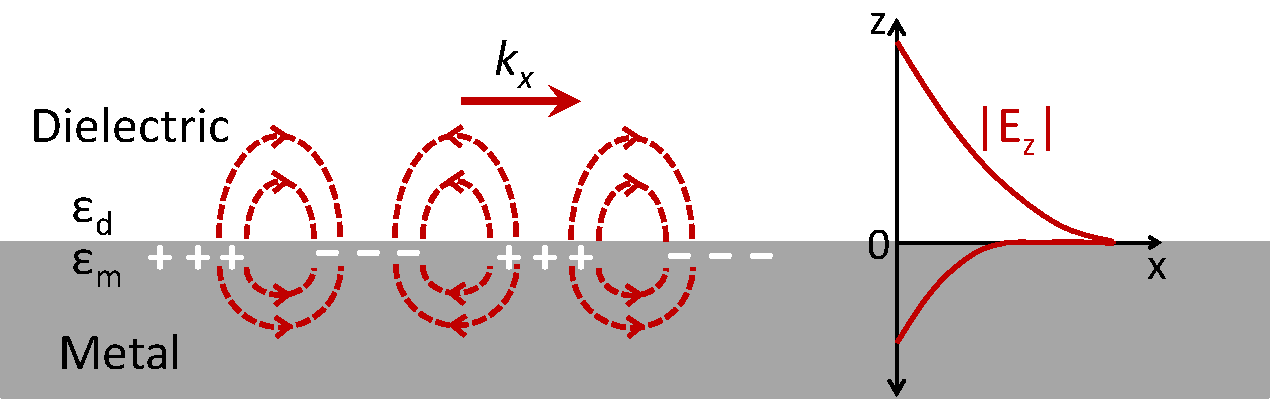
\includegraphics[width=\textwidth]{Fig1}
\caption{Schematic of SPP oscillations at a metal-dielectric surface and the evanescently decaying electric field caused by such plasmons.}
\label{3Fig1}
\end{figure}

Using the geometry of a metal-dielectric interface shown in Fig.\,\ref{3Fig1}, we look for solutions of waves propagation in the $x$ direction but confined to the interface with evanescent decay in the $z$ direction, such that $\vec{\mathbf{E}}(x,y,z)=\vec{\mathbf{E}}(z) e^{i k_x x}$ where $k_x$ is the propagation constant of the wave. We find one set of solutions that is transverse electric (TE) polarised, with the $\vec{\mathbf{E}}$-field component perpendicular to the direction of travel:
\begin{subequations}
\label{TEplasmons}
\begin{align}
H_x &= i \frac{1}{\omega \mu_0} \frac{\partial E_y}{\partial z}\\
H_z &= \frac{k_x}{\omega \mu_0} E_y\\
\frac{\partial^2 E_y}{\partial z^2} &+ (k_0^2 \epsilon_i-k_x^2)E_y = 0 .
\end{align}
\end{subequations}
The subscript $i$ refers to the medium in which the wave is travelling, either $d$ or $m$ for the dielectric and metal respectively. The solutions are waves of the form $e^{i k_x x} e^{k_i z}$. Applying the boundary condition of $E_y$ and $H_x$ continuity across the metal-dielectric interface, we find the condition 
\begin{equation}
\centering
A(k_m+k_d)=0 ,
\label{TEcont}
\end{equation}
where $A$ is the amplitude of wave in the metal halfspace. Since confinement requires Re$(k_m, k_d)>0$, Eq.\,\ref{TEcont} is only fulfilled if $A=0$, i.\,e.\,when no wave can be sustained in the metal. Boundary conditions indicate the wave amplitude of the wave must be 0 in the dielectric as well, thus no SPPs exist in TE polarisation.

The transverse magnetic (TM) polarised solution, with the $\vec{\mathbf{H}}$-field component perpendicular to the direction of travel, is:
\begin{subequations}
\label{TMplasmons}
\begin{align}
E_x &= -i \frac{1}{\omega \epsilon_i \epsilon_0} \frac{\partial H_y}{\partial z}\\
E_z &= -\frac{k_x}{\omega \epsilon_i \epsilon_0} H_y\\
\frac{\partial^2 H_y}{\partial z^2} &+ (k_0^2 \epsilon_i-k_x^2)H_y = 0 \label{TMwave}.
\end{align}
\end{subequations}
Here continuity of $H_y$ and $\epsilon_i E_z$ across the interface requires
\begin{equation}
\centering
\frac{k_d}{k_m} = -\frac{\epsilon_d}{\epsilon_m} ,
\label{TMcont}
\end{equation}
so Re[$\epsilon_m$] and $\epsilon_d$ must be of opposite signs, thus SPPs can only be sustained at a metal-insulator interface. Fulfilment of Eq.\,\ref{TMwave} leads to 
\begin{subequations}
\label{k_relations}
\begin{align}
k_m^2 &= k_x^2-k_0^2\epsilon_m\\
k_d^2 &= k_x^2-k_0^2\epsilon_d ,
\end{align}
\end{subequations}
and combining this with Eq.\,\ref{TMcont} produces
\begin{equation}
\centering
k_x = k_0\sqrt{\frac{\epsilon_m \epsilon_d}{\epsilon_m + \epsilon_d}} ,
\label{SPPdispersion}
\end{equation}
the dispersion relation of an SPP on a metal-dielectric interface. Fig.\,\ref{3Fig2}(a) shows the calculated dispersion for Ag-air SPPs, using a free electron gas model where there is no damping in the metal, i.\,e.\,Im($\epsilon_m)=0$ (values for Ag from Ref.\,\cite{Zeman1987}). The SPP dispersion can be separated into three regions: at frequencies above the plasma frequency of the electron gas $\omega_p$ we have the transparent region ($k_x, k_i$ real) where radiation can penetrate into the metal and excite volume plasmon polaritons. At frequencies below the surface plasmon frequency $\omega_{sp}$ we have bound surface modes ($k_x$ real, $k_i$ imaginary). In the limit $k_x\rightarrow \infty$ plasmons become stationary surface plasmons, where the resonance frequency $\omega_{sp} = \frac{\omega_p}{1+\epsilon_d}$ and $\epsilon_m+\epsilon_d=0$. For $\omega_{sp}<\omega<\omega_p$ no propagating modes exist ($k_x$ imaginary). If damping is included in the metal dielectric, then quasi-bound modes can exist in this intermediate region [Fig.\,\ref{3Fig2}(b), calculated using Ag values from Ref.\,\cite{Johnson1972}]. Note damping introduces a finite maximum $k_x$ for the SPP, leading to a finite propagation length $L_x = \frac{1}{2\textnormal{Im}(k_x)}$, typically on the order $10-100\,\mu$m at visible wavelengths for Au/Ag \cite{Maier2007}. The limit in $k_x$ also produces an upper limit in $k_i$ [Eq.\,\ref{k_relations}], thus limiting the skin depth $L_z = \frac{1}{\textnormal{Im}(k_i)}$ to $\sim10$\,nm in metals. 
\begin{figure}[h!] 
\centering    
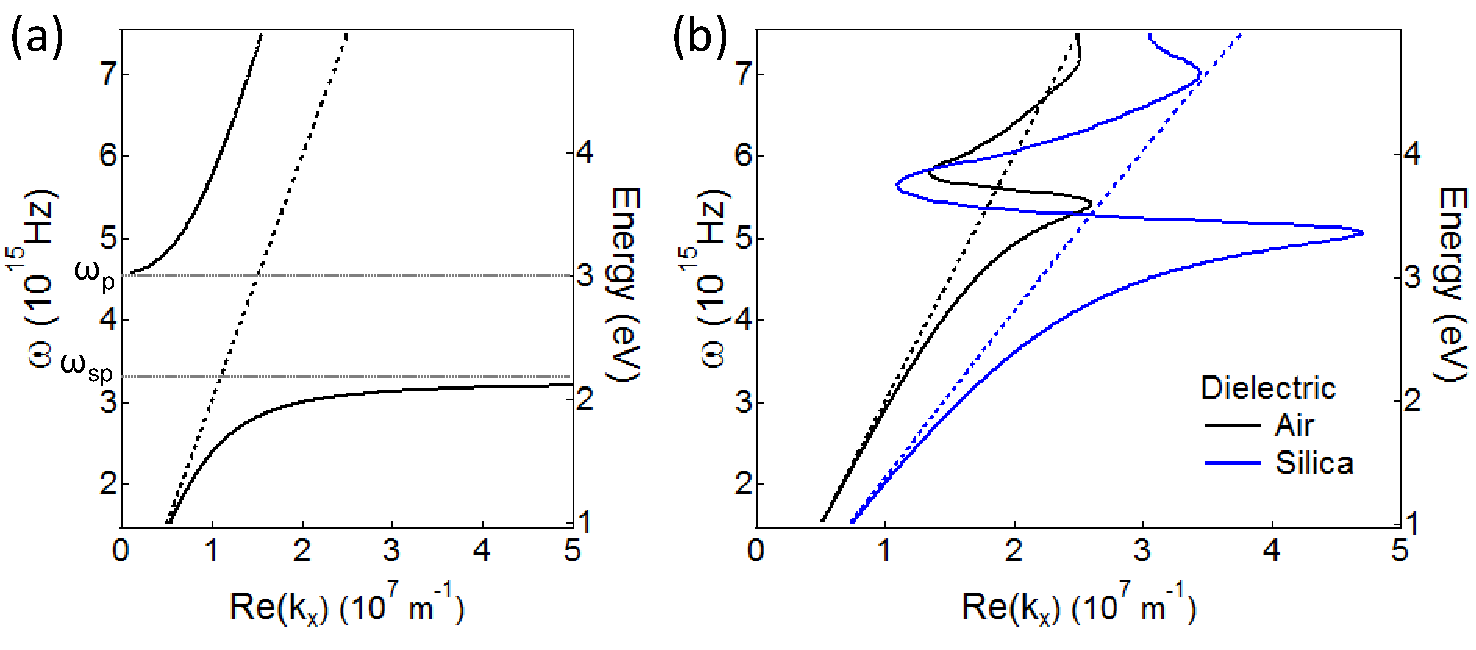
\includegraphics[width=\textwidth]{Fig2}
\caption{Dispersion of SPPs on (a) Ag free electron gas-air and (b) Ag-air/silica interfaces as labelled (solid lines). Light lines in the dielectric are shown by dashed lines. Values for the dielectric function of Ag are taken from Ref.\,\cite{Zeman1987} for (a), and \cite{Johnson1972} for (b).}
\label{3Fig2}
\end{figure}


\section{Plasmonic gratings}
\label{sec:plasmonicgratings}
\begin{figure}[h!]
\centering
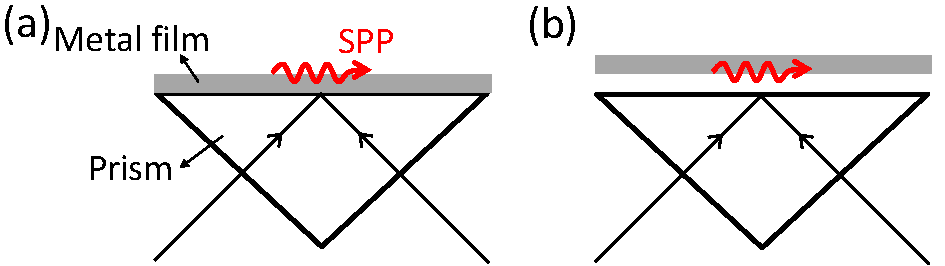
\includegraphics[width=0.8\textwidth]{PrismCoupling}
\caption{Prism coupling to surface plasmon polaritons in the (a) Kretschmann and (b) Otto configurations.}
\label{PrismCoupling}
\end{figure}
The momentum mismatch between SPPs and photons in a dielectric [Fig.\,\ref{3Fig2}] means that it is not possible to directly optically excite SPPs. Instead we must use a phase matching technique, for example prism or grating coupling. In prism coupling a three-layer system is employed either in the Kretschmann or Otto configurations [Fig.\,\ref{PrismCoupling}], in both cases the evanescent field of photons in a higher refractive index material has sufficient momentum to excite SPPs on the interface between a metal and lower refractive index material. In grating coupling, momenta $\hbar\frac{2\pi}{D}m = \hbar G_m$ (integer $m$) can be provided by standing waves set up in a structure with periodicity $D$, thereby allowing photons to couple to SPPs. However in a periodic plasmonic nanostructure SPPs can interact with diffracted photons to produce complex optical spectra, which will be discussed below.

\subsection{First order modes}
\begin{figure}[h!] 
\centering    
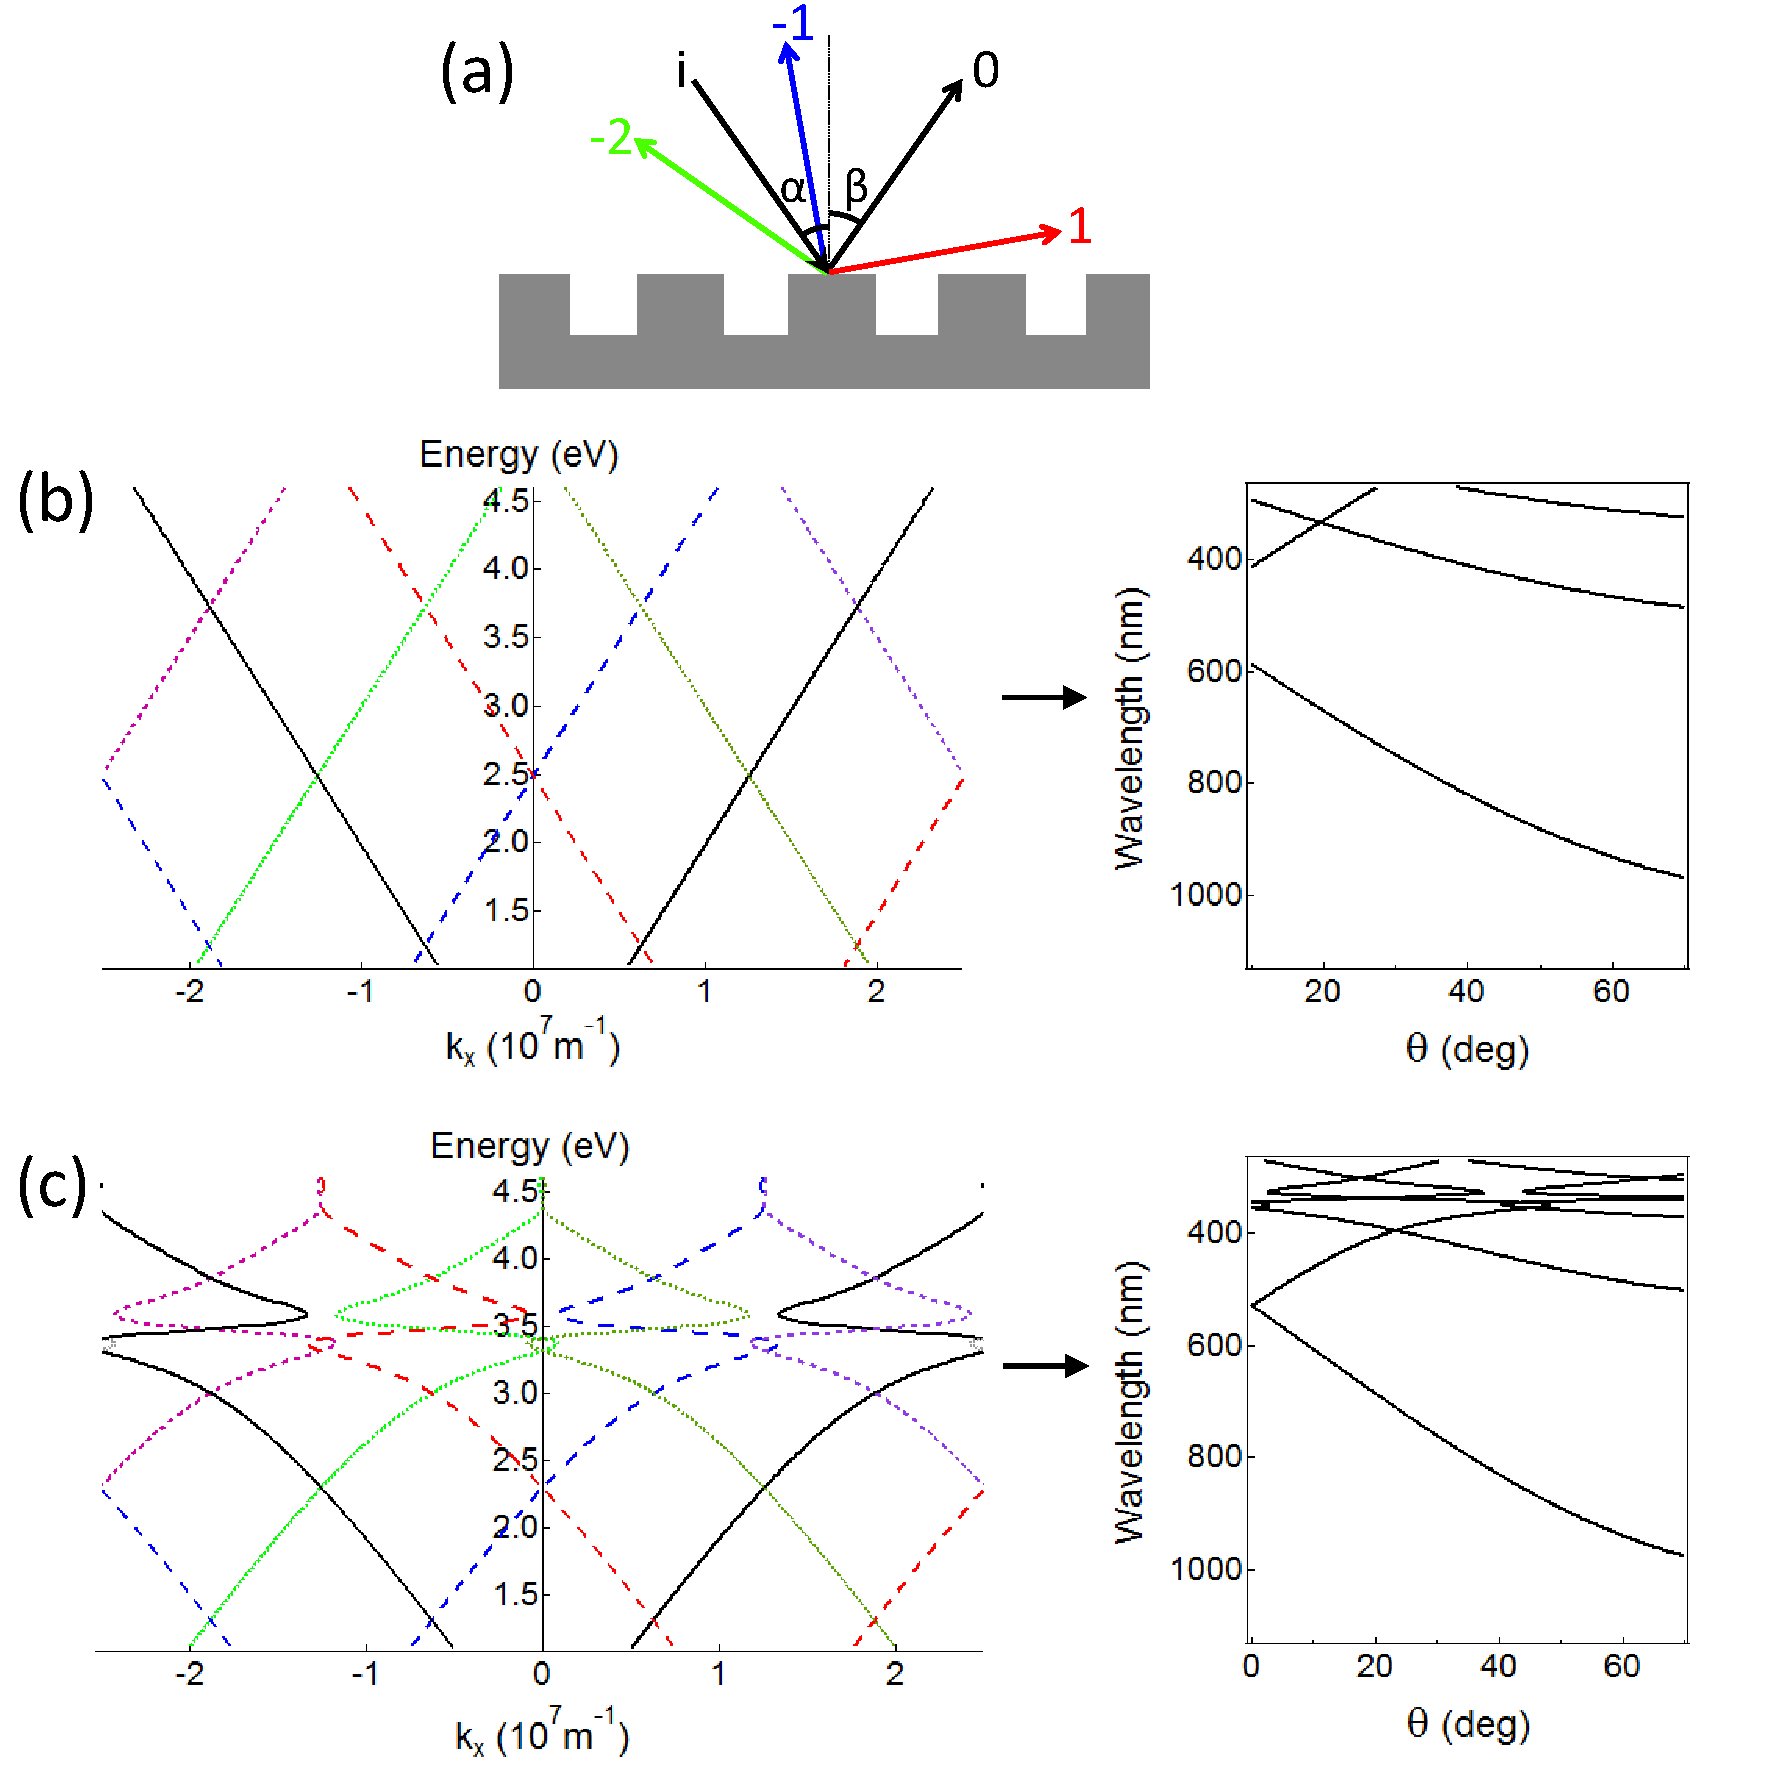
\includegraphics[width=\textwidth]{Fig3}
\caption{(a) Diffraction from a 1D grating structure, showing the incident light and diffracted orders. Dispersion (left) and mode positions in specular reflection as a function of incidence angle $\theta$ (right) for (b) photonic and (c) plasmonic first order modes on $D=500$\,nm Ag grating.}
\label{3Fig3}
\end{figure}
Using Huygens' construction and considering each point on the grating as a wave scatterer, we reach the well-known grating equation for constructive interference
\begin{equation}
\centering
D(\sin\alpha-\sin\beta) = n\lambda ,
\label{GratingEq}
\end{equation}
where $\alpha$ is the angle of incidence and $\beta$ the diffracted angle with respect to the grating normal, $\lambda$ is the wavelength and $n$ the order of the diffracted light [Fig.\,\ref{3Fig3}(a)]. From here we will only consider the zeroth diffraction order (specular reflection) with incidence angle $\theta$ and azimuthal angle $\phi$. In the first order approximation we assume no interactions between diffracted fields, and can distinguish between two types of gratings modes: `photonic' modes caused purely by the interference of light, and `plasmonic' modes where SPPs are excited on the surface of the grating. We can find the dispersion of such grating modes by considering momentum and energy conservation of incoming/outgoing photons, and find
\begin{equation}
\centering
k = k_i^2\sin^2\theta+G_m^2\pm2k_iG_m\sin\theta\cos\phi ,
\label{GratingDisp}
\end{equation}
where the $m$ labels the grating vector $G_m$ needed for momentum matching. Here
\begin{subequations}
\label{kmodes}
\begin{align}
\centering
k_i &= \frac{\omega}{c}\sqrt{\epsilon_d}& \\
k&=\frac{\omega}{c}& \textnormal{(photons) } \label{kphot} \\
k &= \frac{\omega}{c}\sqrt{\frac{\epsilon_m\epsilon_d}{\epsilon_m+\epsilon_d}}& \textnormal{(SPPs) .} \label{kspp}
\end{align}
\end{subequations}
In this case the grating can be thought of as a 1D photonic crystal, where the photon and SPP dispersions are displaced by multiples of the grating vector $G_1$ [Fig.\,\ref{3Fig3}(b,c)]. Different SPP modes on the metal surface can strongly couple and create anticrossings in spectra \cite{Chen1983}.


\subsection{Grating anomalies}
Anomalies are sharp changes in the response of a grating, and first observed by Wood, who noted ``that under certain conditions the drop from maximum illumination to minimum...occurred within a range of wave-lengths not greater than the distance between sodium lines" \cite{Wood1902}. So called Wood's anomalies are second order effects, where interactions between diffracted fields are taken into account. In plasmonic gratings we can further separate this phenomenon into threshold (sharp changes in intensity) and resonance anomalies (dip in intensity at higher wavelength) [Fig.\,\ref{3Fig4}].
\begin{figure}[h!] 
\centering    
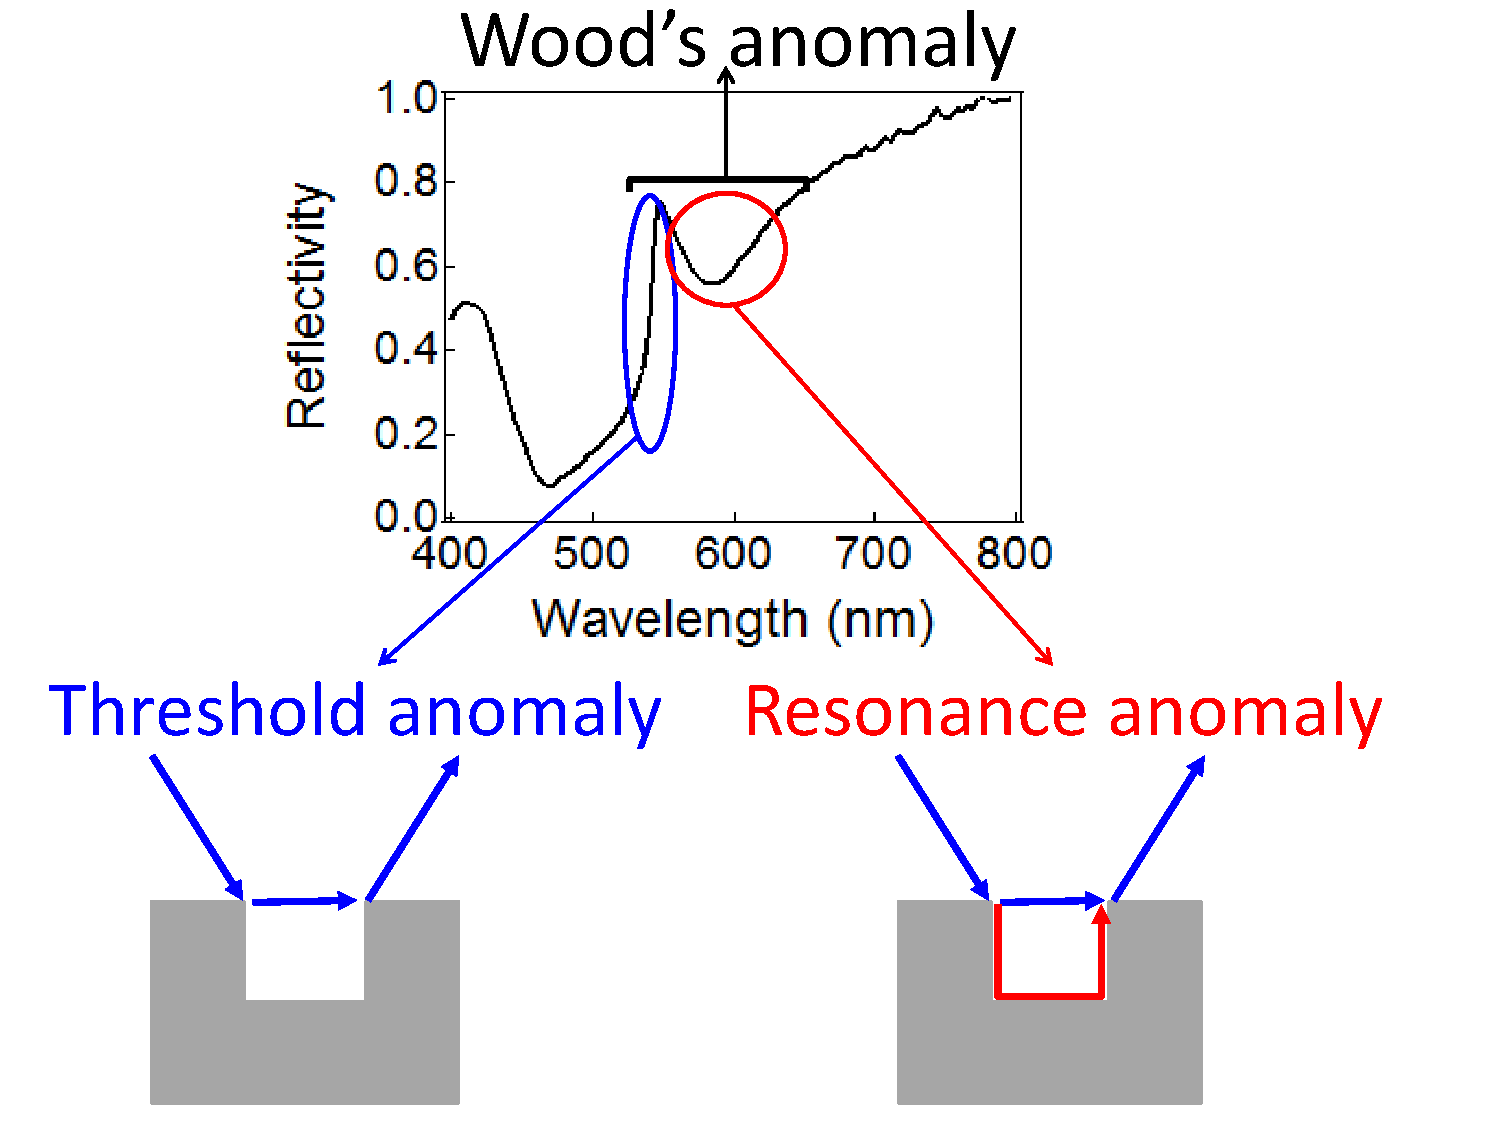
\includegraphics[width=0.7\textwidth]{Fig4}
\caption{Wood's anomaly in the TM-polarised specular reflectivity of Ag grating, $D=417$\,nm. Illustrations of the threshold and resonance anomaly processes are included.}
\label{3Fig4}
\end{figure}

The threshold anomaly is a photonic effect, and comes about when an order is diffracted along the surface of the grating ($\beta=90^{\circ}$). If the order becomes evanescent then the energy available will be redistributed to other diffractive orders. Thus the `passing' order on the edge between diffraction ($\beta<90^{\circ}$) and evanescence ($\beta>90^{\circ}$) causes a sharp change in the diffraction intensity of other diffractive orders, and are observed in the positions of first order photonic modes [Eq.\,\ref{GratingDisp}]. Threshold anomalies can be observed in both polarisations, but generally anomaly strength (i.\,e.\,the difference between maximum and minimum intensity) is smaller in TE polarisation, particularly in metals. In this case the $\vec{\mathbf{E}}$ field is parallel to grating lines and cannot be sustained, leading to less energy redistribution, and a reduction in the effect. Threshold anomalies can be observed in both reflection and transmission gratings, and are responsible for the extraordinary transmission seen in 1D and 2D hole arrays \cite{Fano1941, Hessel1965, Lee2005, Lochbihler1994, Ritchie1968, Treacy2002, Watts1997}.

The resonance anomaly is a plasmonic effect, and comes from an interaction between diffracted light and excited surface waves on the grating. The addition of the SPP oscillator and background photonic diffraction produces a Fano resonance, the asymmetric lineshape in Fig.\,\ref{3Fig4}. Clearly resonance anomalies can only be observed in geometries where SPPs can be excited, e.\,g.\,TM polarisation $\phi=0^{\circ}$, TE polarisation $\phi=90^{\circ}$. The dip position and linewidth depend on the nature of the SPP and is sensitive to the grating profile and material roughness [Fig.\,\ref{3Fig5}]. Therefore we cannot use analytical equations to make predictions about the positions of resonance anomalies, instead we need to use electromagnetic theory to model the grating (see Refs.\,\cite{Hutley1982, Loewen1997} and references therein). In the same way, overcoatings on gratings affect the electromagnetic field near the surface and can change the position and strength of anomalies, particularly resonance anomalies. In addition, modes excited in the coating material can change the $\vec{\mathbf{E}}$ field polarisation and excite anomalies in previously forbidden geometries \cite{Hutley1982, Loewen1997}.
\begin{figure}[h!] 
\centering    
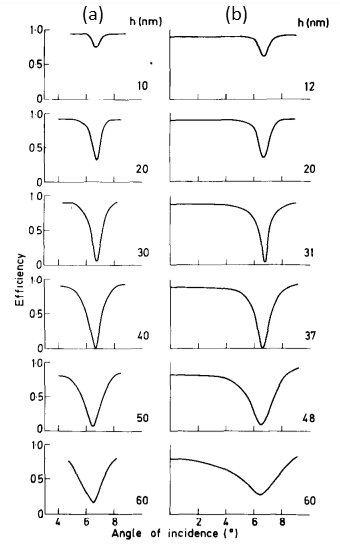
\includegraphics[width=0.6\textwidth]{Fig5}
\caption{(a) Electromagnetic theory modelling and (b) experimental dependence of resonance anomaly on the grating depth $h$ for $D=556$\,nm sinusoidal Au grating at $\lambda=647$\,nm \cite{Hutley1976}. }
\label{3Fig5}
\end{figure}


\subsection{Localised and guided modes}
Gratings can also give rise to optical modes that do not rely on diffraction. In particular the grating slits are independent open electromagnetic waveguides that can sustain TE and TM modes. For example, the dispersion of a TE$_{\mu\nu}$ mode is \cite{Jackson1999}
\begin{equation}
\centering
\frac{\omega^2}{c^2}(n_{\mathit{eff}}^2-\sin^2\theta) = \pi^2\left(\frac{\mu^2}{a_{\mathit{eff}}^2}+\frac{\nu^2}{b_{\mathit{eff}}^2}\right) ,
\label{waveguide}
\end{equation}
where $n_{\mathit{eff}}$ is the effective refractive index experienced by the mode in the grating slit, $a_{\mathit{eff}}$ the effective cavity width and $b_{\mathit{eff}}$ the effective cavity height, and $\mu, \nu$ are indices used to label the waveguide mode. Due to the penetration of electromagnetic fields in metals, $a_{\mathit{eff}}$ is not the same as the geometric width of the grating slit, and particularly if there is a coating on the metal then $a_{\mathit{eff}}$ and $b_{\mathit{eff}}$ both have some dependence on $n_{\mathit{eff}}$. 

If SPPs are excited, then grating slits can be thought of as a metal/insulator/metal waveguide. SPPs travelling on slit edges can interact to form symmetric and antisymmetric combinations, particularly if the slit is narrow \cite{Maier2007}. For rectangular slits, often known as trench waveguides, the highest $\vec{\mathbf{E}}$ field intensity is at the top corners of slits and thus extends outside the groove [Fig.\,\ref{3Fig6}(a), right] \cite{Bozhevolnyi2005, Srivastava2009, Chattopadhyay2012}. For V-shaped slits, the gradual change in width leads to multiple reflections, and localisation of the $\vec{\mathbf{E}}$ field at the bottom of the grooves (adiabatic nanofocusing) [Fig.\,\ref{3Fig6}(a), left] \cite{Bozhevolnyi2005, Srivastava2009, Novikov2002, Kuttge2009, Sondergaard2012}. These modes are called channel plasmon polaritons (CPPs) and can be observed in near-field optical microscopy [Fig.\,\ref{3Fig6}(b)]. Due to their localised nature, CPPs can be distinguished from diffractive grating modes by their relatively flat dispersions.
\begin{figure}[h!] 
\centering    
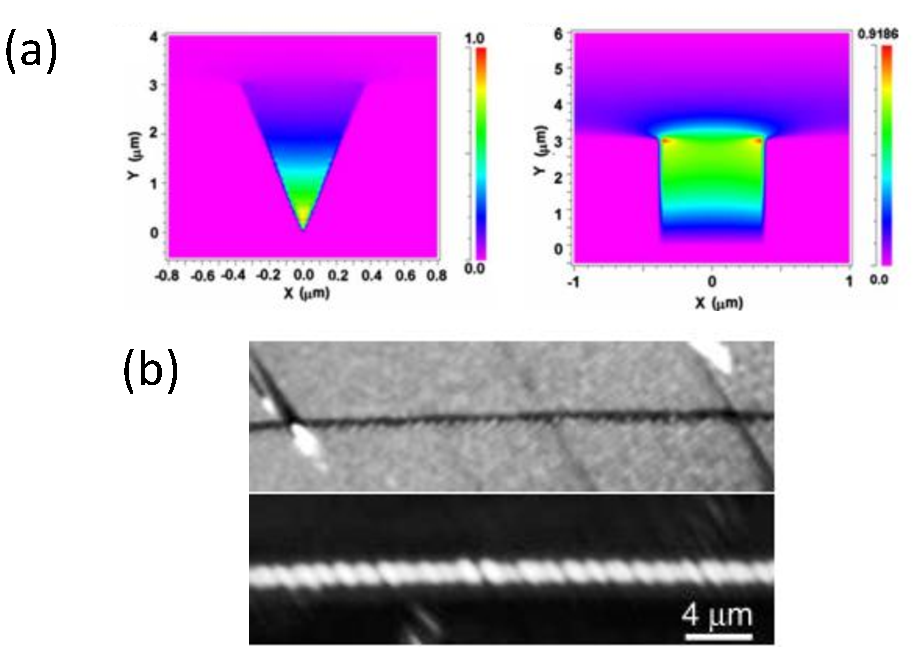
\includegraphics[width=0.8\textwidth]{Fig6}
\caption{(a) $\vec{\mathbf{E}}$ field profiles of channel plasmon polariton modes in a V-shaped (left) and trench (right) Au groove, with width 3.75\,$\mu$m and depth 3\,$\mu$m filled with air \cite{Srivastava2009}. (b) Topographical (top) and near-field optical images (bottom) for V-shaped Au slit with width 0.6\,$\mu$m and depth 1\,$\mu$m at $\lambda=1440$\,nm. Interference can be seen in the near-field image as a result of interference with scattered light \cite{Bozhevolnyi2005}.}
\label{3Fig6}
\end{figure} 

\section{Localised surface plasmons}
\subsection{Quasi-static approximation}
For a spherical nanoparticle (NP) whose diameter $d\ll\lambda$, the phase of the $\vec{\mathbf{E}}$ field is approximately constant across the particle and we can solve the simplified problem of a sphere in an electrostatic field, then include the harmonic time dependence as a last step. The geometry is shown in Fig.\,\ref{3Fig7}(a), with a homogeneous metal particle (dielectric function $\epsilon_m$) of diameter $d$ at the origin inside a dielectric medium $\epsilon_d$, and $\vec{\mathbf{E}} = E_0\vec{z}$. Solving the Laplace equation for the potential $\Phi$ ($\vec{\mathbf{E}} = -\nabla\Phi$), we find
\begin{subequations}
\label{NPlaplace}
\begin{align}
\Phi_{in} &= -\frac{3\epsilon_d}{\epsilon_m+2\epsilon_d}E_0r\cos\theta \label{PhiIn}\\
\Phi_{out} &= -E_0r\cos\theta+\frac{\epsilon_m-\epsilon_d}{\epsilon_m+2\epsilon_d}E_0\left(\frac{d}{2}\right)^3\frac{\cos\theta}{r^2} \label{PhiOut}
\end{align}
\end{subequations}
at a distance $r$ from the centre of the sphere, where $\Phi_{in}$ and $\Phi_{out}$ represent the potentials inside and outside the sphere respectively. From Eq.\,\ref{PhiIn} we can see that the potential and electric field is enhanced at the NP surface by factor of $\frac{3\epsilon_d}{\epsilon_m+2\epsilon_d}$ as a result of the induced surface charges [Fig.\,\ref{3Fig7}(c)]. This effect also appears in Eq.\,\ref{PhiOut}, which is the superposition of the applied field $E_0$ and an induced dipole in the NP with dipole moment $\vec{p}$ and polarisability $\alpha$, such that
\begin{subequations}
\label{NPdipole}
\begin{align}
\vec{p} &=4\pi\epsilon_0\epsilon_d\left(\frac{d}{2}\right)^3\frac{\epsilon_m-\epsilon_d}{\epsilon_m+2\epsilon_d}\vec{\mathbf{E}} \label{NPmoment}\\
\alpha &= 4\pi\left(\frac{d}{2}\right)^3\frac{\epsilon_m-\epsilon_d}{\epsilon_m+2\epsilon_d} \label{NPpolarisability} .
\end{align}
\end{subequations}
A resonance in $\alpha$ is achieved when 
\begin{equation}
\centering
\epsilon_m(\omega) = -2\epsilon_d(\omega) ,
\label{Frolich}
\end{equation}
known as the Fr\"{o}lich condition, and provides the resonance frequency of the dipolar localised surface plasmon (LSP) for a metallic NP. For a free electron gas in air, this condition is achieved at $\omega = \frac{\omega_p}{\sqrt{3}}$, but will clearly depend on both $\epsilon_m$ and $\epsilon_d$. For this reason the LSP resonance of Ag NPs is at a higher frequency than Au NPs with the same $d$ [Fig.\,\ref{3Fig7}(b)]. Note the asymmetric shape of the Au extinction peak due to the onset of interband transitions. The harmonically oscillating $\vec{\mathbf{E}}$ field acts to drive electron oscillations in the NP, and causes a large field enhancement in the vicinity of the particle in the same way as an SPP [Fig.\,\ref{3Fig7}(c)]. For NP arrays, if particles are separated by $\gtrsim2d$ then LSP fields do not interact \cite{Rechberger2003}.
\begin{figure}[h!] 
\centering    
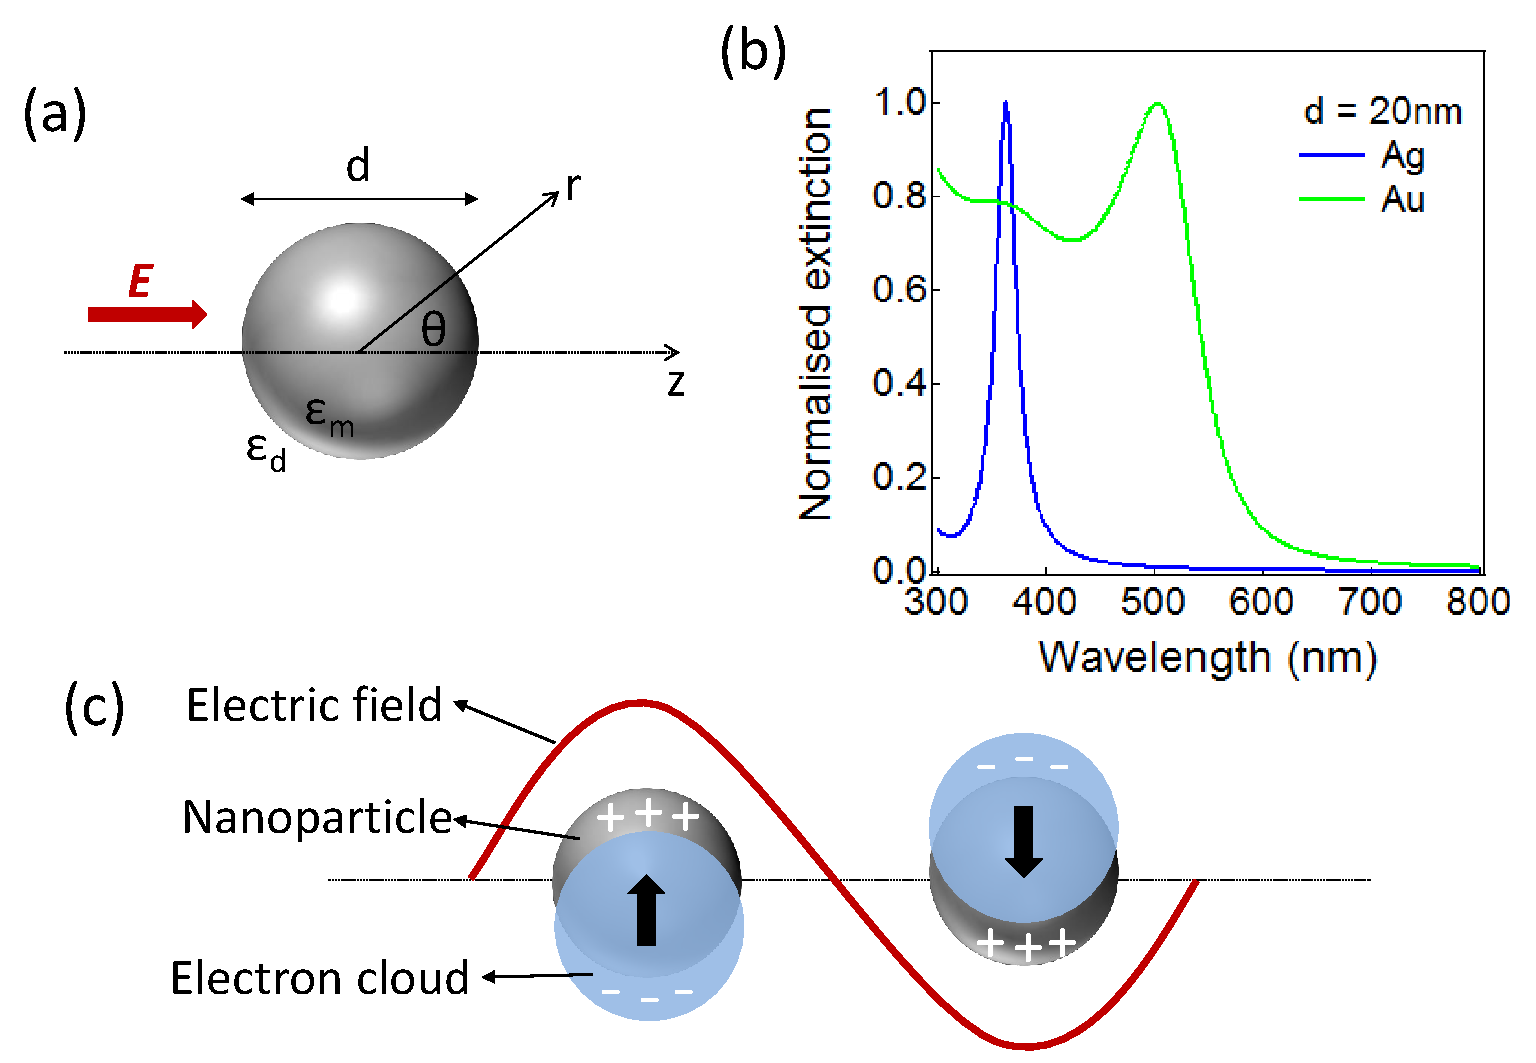
\includegraphics[width=0.8\textwidth]{Fig7}
\caption{(a) Geometry used to calculate the localised surface plasmon resonance of a homogeneous metal sphere with diameter $d$ placed inside a electrostatic $\vec{\mathbf{E}}$ field. (b) Normalised extinction spectra for $d=20$\,nm Ag/Au NPs in air. (c) Schematic of dipolar electron oscillations in NPs driven by an electric field.}
\label{3Fig7}
\end{figure} 

The oscillating NP dipole leads to radiation, which can be seen as the scattering of light from the NP. The scattering $C_{\mathit{scat}}$ and absorption $C_{\mathit{abs}}$ cross sections of the particle are given by
\begin{subequations}
\label{NPcrossSections}
\begin{align}
C_{\mathit{scat}} &= \frac{k^4}{6\pi}|\alpha|^2 = \frac{8\pi}{3}k^4\left(\frac{d}{2}\right)^6 \left|\frac{\epsilon_m-\epsilon_d}{\epsilon_m+2\epsilon_d}\right|^2 \label{Scat}\\
C_{\mathit{abs}} &= k\textrm{Im}[\alpha] = 4\pik\left(\frac{d}{2}\right)^3\textrm{Im}\left[\frac{\epsilon_m-\epsilon_d}{\epsilon_m+2\epsilon_d}\right] \label{abs} ,
\end{align}
\end{subequations}
and we define extinction $C_{\mathit{ext}} = C_{\mathit{scat}}+C_{\mathit{abs}}$. The resonance in $\alpha$ gives rise to a maximum in the optical response of the NP. For very small NPs absorption dominates over scattering due to its $d^3$ dependence, for example for $d=30$\,nm Ag NPs the extinction is almost entirely due to absorption, while the reverse is true for $d=90$\,nm [Fig.\,\ref{3Fig8}].
\begin{figure}[h!] 
\centering    
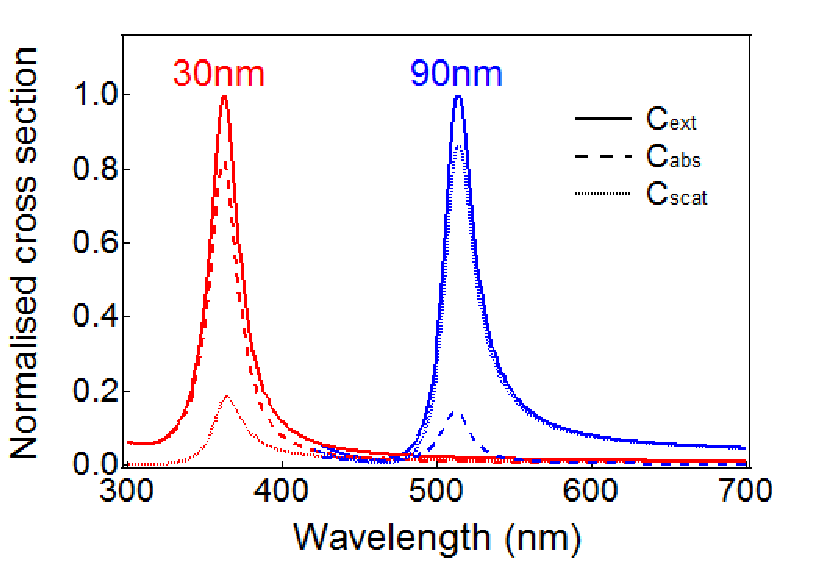
\includegraphics[width=0.8\textwidth]{Fig8}
\caption{Normalise absorption (dashed lines), scattering (dotted lines) and extinction (solid lines) cross sections for Ag NPs $d=30$, 90\,nm at $\lambda=500$\,nm in air according to Eq.\,\ref{NPcrossSections}. The $d=90$\,nm data has been shifted for clarity.}
\label{3Fig8}
\end{figure}

\subsection{Size and shape effects}
The quasi-static approximation models the NP as an electric dipole whose resonance frequency depends purely on the relative dielectric functions of the metal and surrounding medium. The underlying assumption that the phase of the $\vec{\mathbf{E}}$ field across the particle is constant is only true for very small particles, and works well for $d<50$\,nm Ag particles [Fig.\,\ref{3Fig9}]. For larger particles an electrodynamic model must be used, for example Mie theory, where the electromagnetic field is separated into subfields made of infinite series of of partial waves with spherical polar geometry. Applications of boundary conditions and Maxwell's equations leads to a set of differential equations that can be solved to find the form of LSP fields. Mie theory produces a redshift in LSP resonance with $d$ as seen in experiment, as well as the emergence of multipole modes for larger particles [Fig.\,\ref{3Fig9}(a)] \cite{Maier2007, Born1999}. For example in Ag particles, the quadrupole mode is first observed as a shoulder in the extinction spectrum for $d=90$\,nm particles. [Insert sentence about form of dipole/quadrupole fields.]
\begin{figure}[h!] 
\centering    
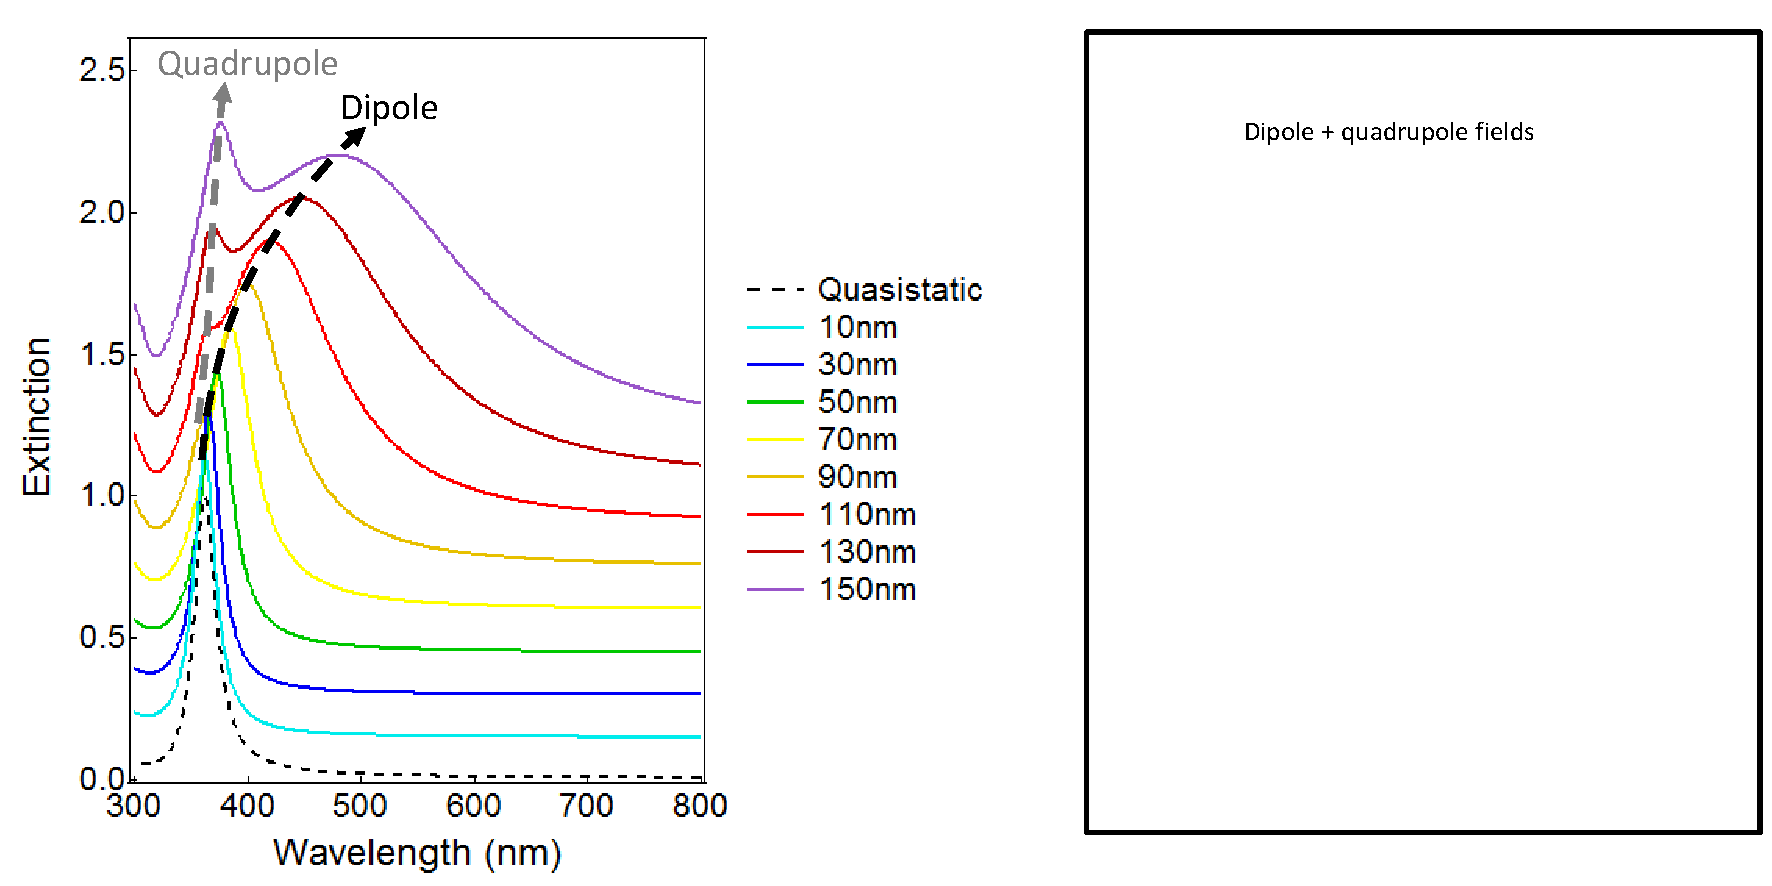
\includegraphics[width=\textwidth]{Fig9}
\caption{Calculated extinction spectra for NPs with labelled $d$ in air using Mie theory, normalised to the dipole maximum and offset for clarity. The quasi-static approximation resonance is added for comparison.}
\label{3Fig9}
\end{figure}

The resonance of NPs is also very sensitive to the particle shape, and both quasi-static and Mie theory calculations can be adapted for non-spherical geometry. This provides great tunability in the LSP wavelength via control of particle growth. Deviations from spherical geometry leads to the production of multiple redshifted peaks [Fig.\,\ref{3Fig10}(a)]. In the case of nanorods, we observe two LSP resonances in unpolarised spectra: a transverse mode associated with electron oscillations along the short axis, and a longitudinal mode related to electron oscillations along the long axis. The longitudinal resonance wavelength depends on the aspect ratio of the nanorod [Fig.\,\ref{3Fig10}(b)], and the controllable growth of nanorods is often used to produce a required LSP resonance \cite{Wiley2006, Wiley2007, Chen2013}.
\begin{figure}[h!] 
\centering    
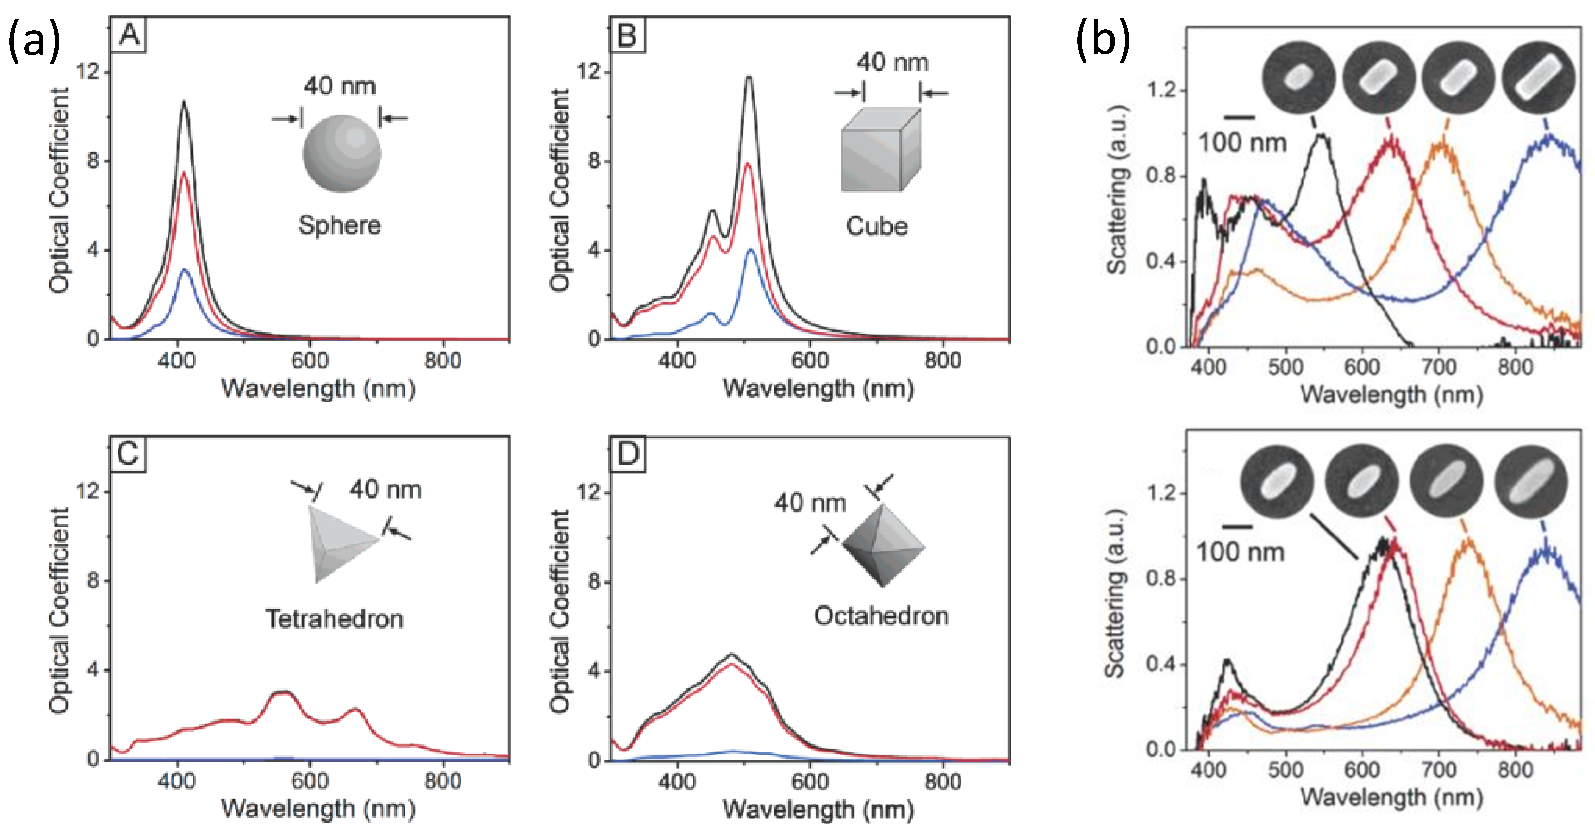
\includegraphics[width=\textwidth]{Fig10}
\caption{(a) Discrete dipole approximation calculations of the extinction (black), absorption (red) and scattering (blue) of Ag nanoparticles with the geometries shown \cite{Wiley2006}. (b) SEM images and normalised scattering spectra of individual Ag nanobar (left) and nanorice (right) structures \cite{Wiley2007}.}
\label{3Fig10}
\end{figure}

\section{Conclusions}
Surface plasmons are collective oscillations of electrons in a metal. Such oscillations show resonance in many geometries, specifically as travelling surface waves on planar metal films, or localised oscillations in metal nanoparticles. The resonance frequency depends on the relative dielectric functions of the metal and surrounding medium, and is very sensitive to the nanostructure geometry. Surface plasmons cause large electric field enhancement around the vicinity of the metal, which can be used to increase optical coupling with materials near the metal surface. Periodic plasmonic nanostructures can sustain many diffractive or guided modes, and zone-folding allows incoming/outgoing light to reach parts of the photon and plasmon dispersions that may not be otherwise accessible, while interactions between electron and photon fields gives rise to sharp changes in intensity called anomalies. The strengths and positions of grating modes can be modified via grating geometry, as well as the polarisation and configuration of incoming light.
%*****************************************************************************************
%*********************************** Fourth Chapter **************************************
%*****************************************************************************************

\chapter{Lead iodide perovskite thin films}

\graphicspath{{Chapter4/Figures/}}

Spin coating is a process that can be used to fabricate thin films on relatively flat substrates. After a solution is deposited, the substrate is accelerated to the desired spin speed and continues rotating to remove excess solution. As the solvent evaporates the material self-assembles to form a solid film. The process is commonly used in industry as it can controllably produce films of thickness 10\,nm to 100\,\textmu m, covering areas with lateral size up to 10\,cm. The film thickness and morphology depend on solution concentration, spin speed and substrate preparation. It is possible to create PbI perovskite films using spin coating [Sec.\,\ref{sec:spin}], however optimisation is required in order to create continuous and uniform films with thickness under 100\,nm. In this Chapter the formation of C$_{12}$PI (\ce{(C12H25NH3)2PbI4}) and CHPI (\ce{(C6H9C2H4NH3)2PbI4}) films spin coated on silica substrates will be explored.

\section{Spin coating theory}
Although spin coating is experimentally simple, it is complicated to model due to the large number of factors involved. Initially, fluid inertia and surface tension are important as the fluid front spreads out in spiral waves. Solvent evaporation also begins at this point, and a small boundary layer is formed at the liquid-gas interface. At the end of this step a thin and even film forms on the substrate. In the next phase a balance between viscous and centrifugal forces causes fluid flow and thinning. The boundary layer in the solution gradually gets thicker, and the solute concentration varies throughout the film thickness. Viscosity rises as a result of solvent evaporation, eventually inhibiting further flow. Further fluid loss is caused by solvent evaporation, which dominates thinning in the latter stages, and eventually solute concentration becomes uniform throughout the film. There is also a small atmospheric boundary layer above the solution that can influence mass transfer and exert shear forces at the interface \cite{Meyerhofer1978, VanHardeveld1995, Lawrence1988}. The initial acceleration may also affect final film thickness, as too slow an acceleration can lead to complete solvent evaporation before the final spin speed is reached \cite{Birnie2005}.

Various approximations have been used in models of spin coating. Meyerhofer considered the solvent evaporation negligible until the mass loss due to rotational forces fell to the level of the evaporation rate \cite{Meyerhofer1978}, van Hardeveld \textit{et al.\,}used the same principles but modelled the evaporation rate more rigorously in terms of rate of mass transfer at the interface \cite{VanHardeveld1995}, and Lawrence took both the solvent and atmospheric boundary layers into consideration\cite{Lawrence1988}. All three models agree that the final film thickness $h_f$ depends on the angular spin speed $\omega$ as $h_f \propto \omega^{-0.5}$, and this relationship has been experimentally verified \cite{Meyerhofer1978, VanHardeveld1995}. However other exponents have been reported, and Lawrence indicated that an exponent %WN
larger %end
than $-0.5$ may be measured in films that complete the full spinning process before reaching $\omega$, and are thus thicker than the calculations anticipate. Shear thinning, where the viscosity of the solution decreases with an increased shear stress, may also be responsible \cite{Lawrence1988}.

\begin{figure}[h!]
\centering    
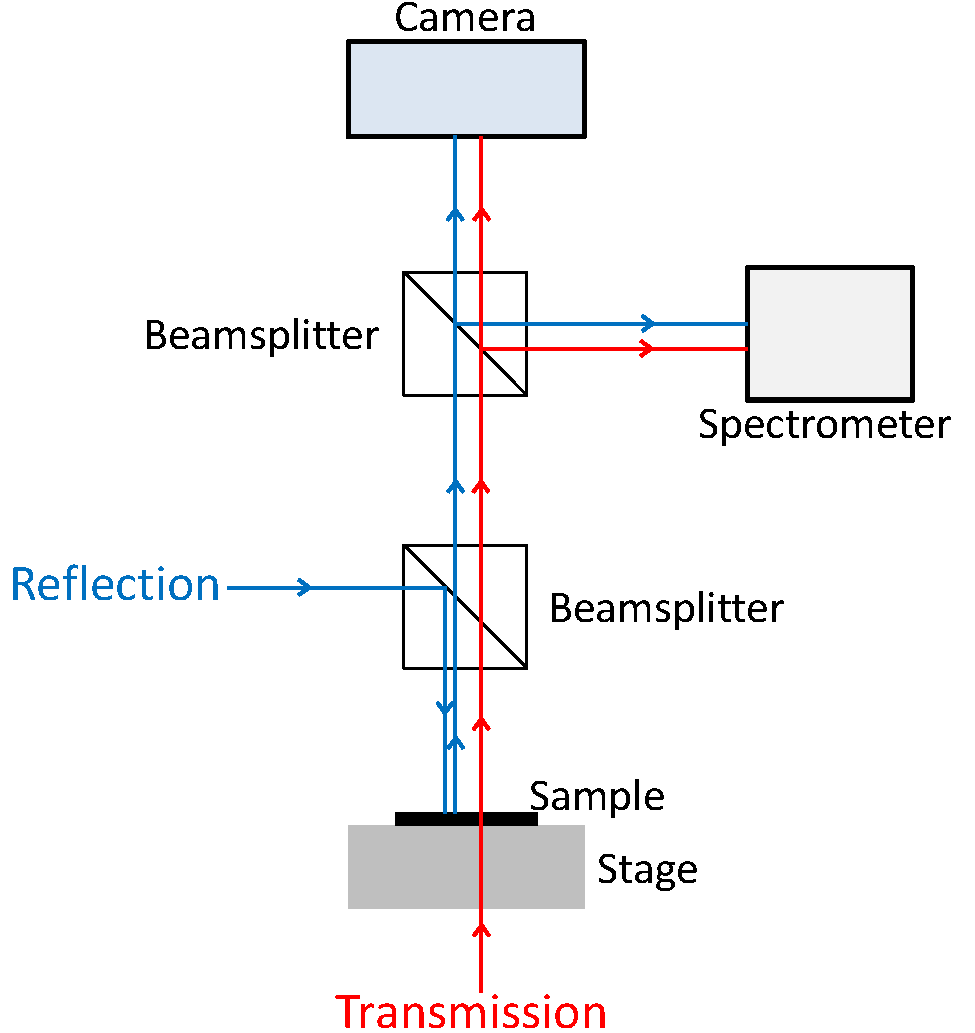
\includegraphics[width=0.6\textwidth]{Microscope}
\caption{Schematic of optical microscopy and spectroscopy setup, including the reflection and transmission beam paths.}
\label{Microscope}
\end{figure}
\section{Experimental methods}
\label{sec:glass}
Spin coating solutions are prepared by dissolving a chemically synthesised perovskite powder [Sec.\,\ref{sec:solutiongrowth}] in tetrahydrofuran (THF) with a concentration of 20\,mg/ml. Silica substrates are sonicated in a four-step process for approximately 15 minutes per solvent: firstly in a deionised water and detergent solution, then in deionised water, acetone, and finally isopropanol. Three additional substrate preparation techniques are investigated in order to create the most uniform films: \\
(1) \ce{CO2} snowjetting, where a high velocity mix of gaseous and solid carbon dioxide is focused on the substrate, cleaning the surface as a result of momentum transfer and solvent action of the \ce{CO2} \cite{Snowjet}. \\
(2) Silanisation, where substrates are dipped in a 2 vol\% solution of aminopropyltriethoxy silane (APTES) in dry acetone for approximately 90 minutes. A self-assembled monolayer of silane molecules forms on the substrate, and in the case of APTES the surface is functionalised with amine groups. \\
(3) Plasma etching, where substrates are treated using a Diener Electronic Femto plasma system for 5 minutes, using an oxygen plasma to clean contaminants from the substrate. The surface is functionalised with hydroxyl groups and becomes more hydrophilic.

Perovskite films are characterised using optical microscopy and spectroscopy (signals are collected over areas with diameter $\approx 20$\,\textmu m unless otherwise specified) [Fig.\,\ref{Microscope}], and the film thickness is determined by atomic force microscopy (AFM) measurements over scratches in the film.

\begin{figure}[h!]
\centering    
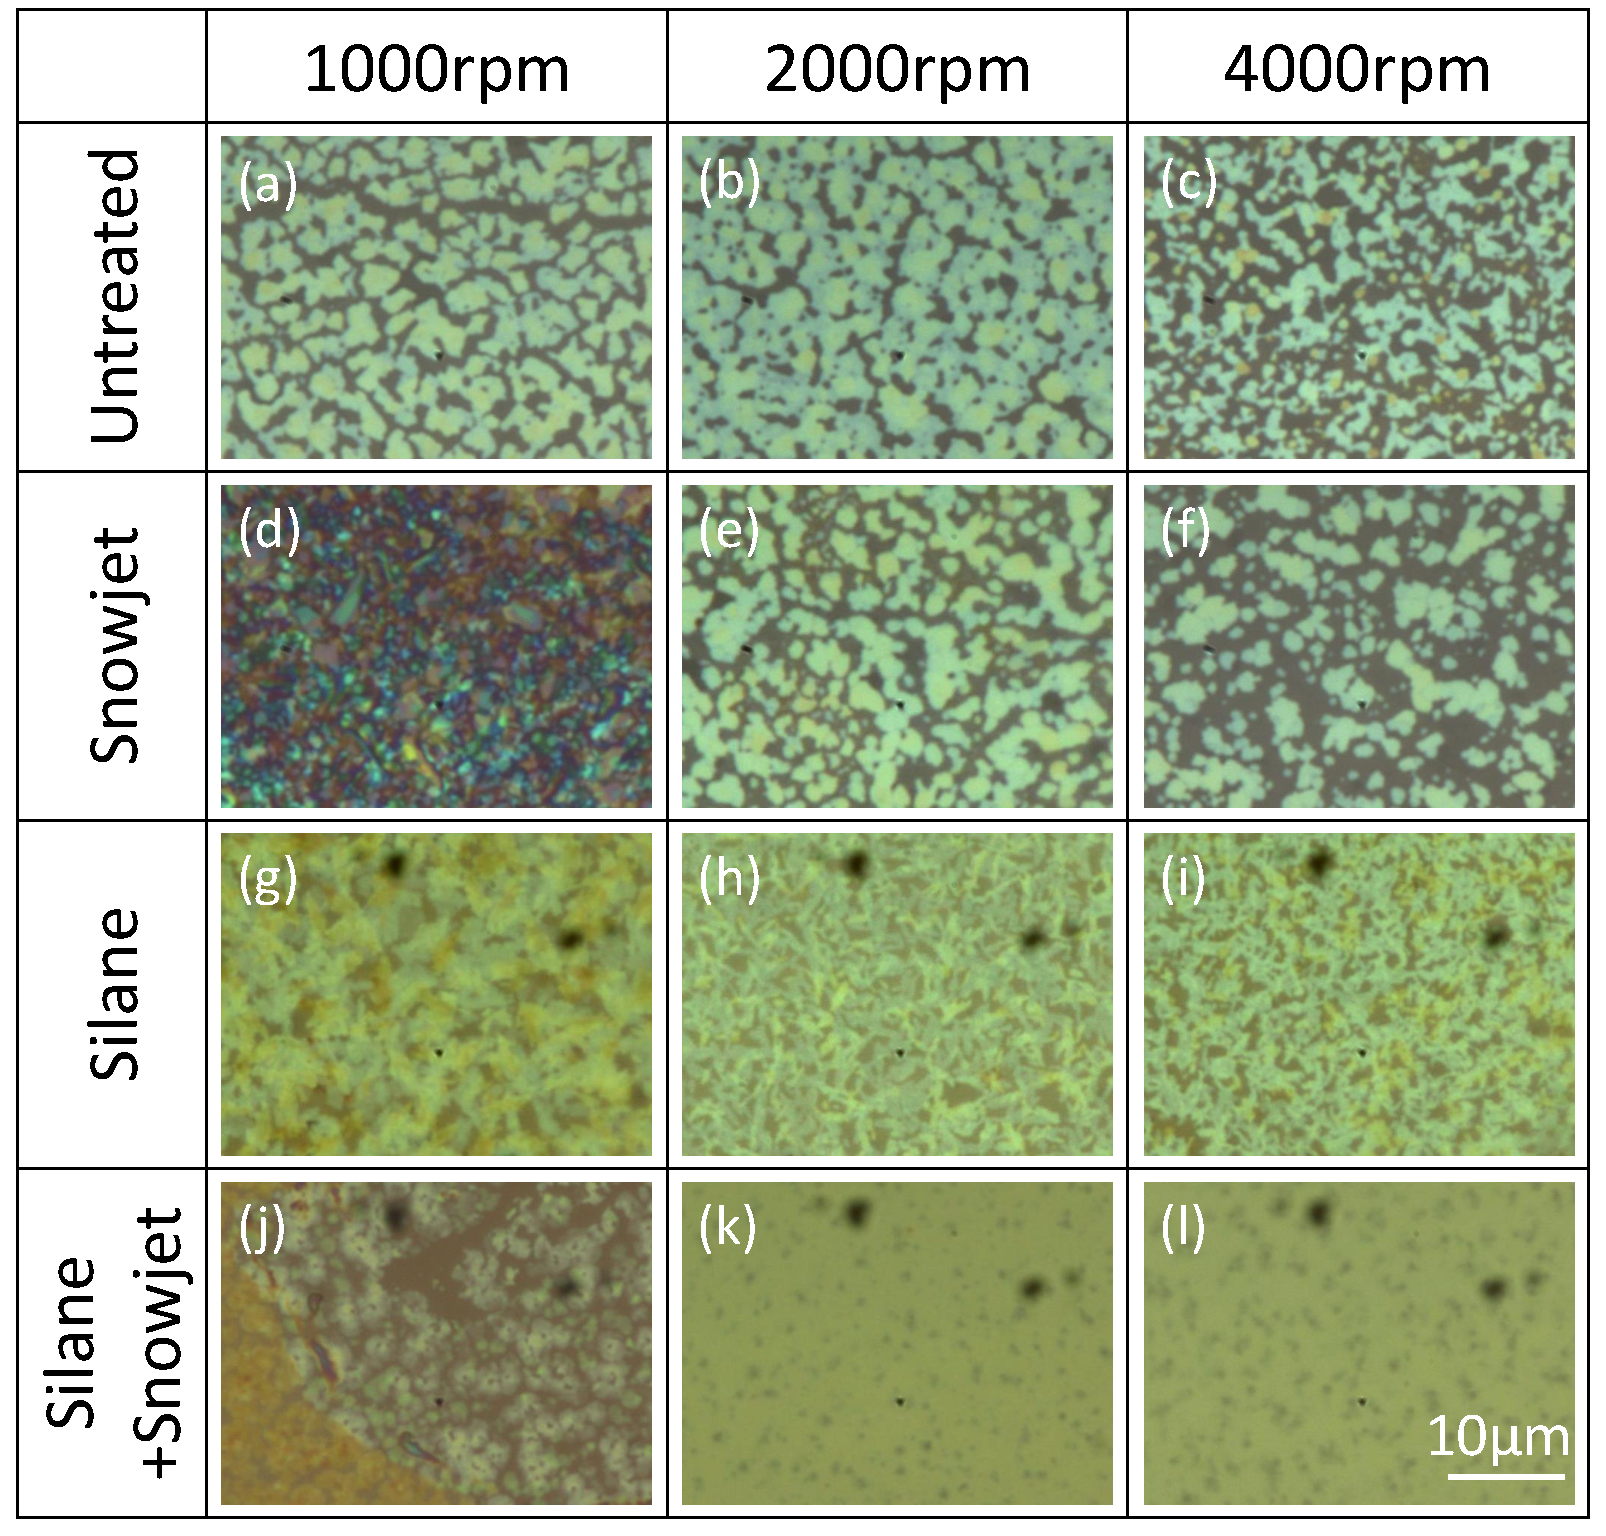
\includegraphics[width=0.88\textwidth]{Fig1}
\caption{BF images at 100$\times$ magnification of spin coated C$_{12}$PI films on silica, with spin speed and substrate preparation as labelled. Note the substrate was heated immediately prior to spin coating for (d). The black marks seen on (g-l) are due to dust particles on the microscope lens.}
\label{4Fig1}
\end{figure}
\section{C$_{12}$PI thin films}
\label{sec:4-1}
Bright field reflection (BF) images of C$_{12}$PI films spin coated on silica at 100$\times$ magnification are shown in Fig.\,\ref{4Fig1}. Due to the hydrophobic nature of the organic molecule, C$_{12}$PI films show significant dewetting without substrate functionalisation [Figs.\,\ref{4Fig1}(a-f)], and for this reason films are not formed on plasma etched substrates (not shown). The non-uniform film in Fig.\,\ref{4Fig1}(d) does not exhibit such dewetting as the substrate was heated before application of the C$_{12}$PI solution, thus the solvent evaporated before excess fluid could be removed. Silanisation increases attractive interactions between constituents of C$_{12}$PI and the substrate, thereby improving film coverage [Figs.\,\ref{4Fig1}(g-i)]. A further snowjet step removes excess APTES that may remain after silanisation, reducing surface roughness and producing the most uniform C$_{12}$PI samples [Figs.\,\ref{4Fig1}(k,l)].

\begin{figure}[h!]
\centering
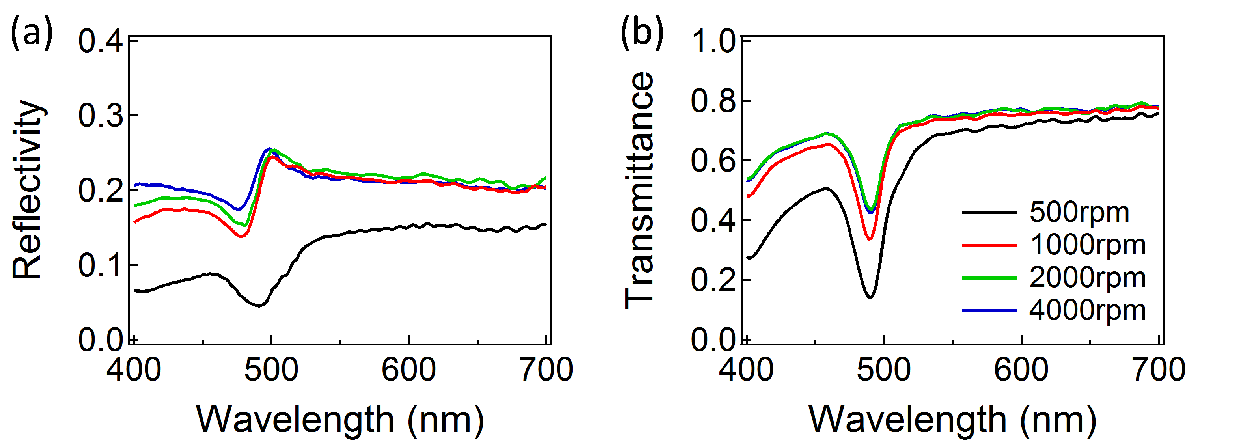
\includegraphics[width=\textwidth]{Fig2}
\caption{(a) Reflection and (b) transmission spectra for C$_{12}$PI films on silanised silica substrates.}
\label{4Fig2}
\end{figure}
\subsection{Spin speed}
\label{sec:4-2}
Optical spectra of C$_{12}$PI films created on silanised substrates illustrate the general trends observed for all substrate preparations [Fig.\,\ref{4Fig2}]. The exciton appears as a Fano resonance at the expected wavelength of 490\,nm \cite{Pradeesh2009} in reflectivity due to interference between its narrow resonance and the continuum background, while a dip appears in the transmittance spectra due to exciton absorption. Although both phases of C$_{12}$PI are observed for films below 2000\,rpm [Sec.\,\ref{sec:Cnphases}], here we consider only the high energy exciton. Spectra can be directly correlated to the BF images, hence increased roughness observed in 500\,rpm films translate to a lowering of the overall reflectivity as a result of scattering. In the same way, similarities in the morphologies of films made above 1000\,rpm [Figs.\,\ref{4Fig1}(g-i)] lead to almost identical optical spectra. As C$_{12}$PI is a multilayer system, more excitons are available for absorption as the film thickness increases, thus the amplitude of the exciton dip in transmission spectra can be used as a gauge of the film thickness. From Fig.\,\ref{4Fig2}(b) we see that the film thickness decreases with spin speed as expected.

\begin{figure}[h!]
\centering
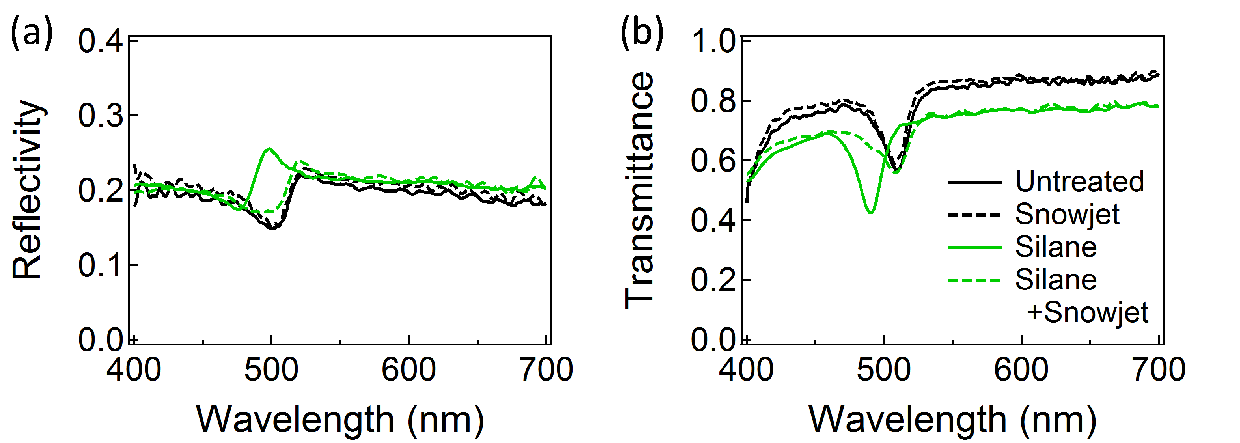
\includegraphics[width=\textwidth]{Fig3}
\caption{(a) Reflection and (b) transmission spectra for C$_{12}$PI films spin coated on silica at 4000\,rpm.}
\label{4Fig3}
\end{figure}
\subsection{Substrate preparation}
\label{sec:4-3}
Optical spectra of 4000\,rpm C$_{12}$PI films made using a variety of substrate preparation techniques are shown in Fig.\,\ref{4Fig3}. The reflectivity spectra are almost identical for all substrate preparations [Fig.\,\ref{4Fig3}(a)], with the exception of the silanised substrate where excess APTES molecules led to increased surface roughness, thus favouring the more crumpled and higher energy C$_{12}$PI phase. Removal of the excess silane via snowjetting creates flatter inorganic sheets and lowers the exciton energy. Dewetting of C$_{12}$PI films on non-functionalised substrates produces an increase in the film transmittance away from the exciton resonance [Fig.\,\ref{4Fig3}(b)].

\begin{figure}[h!]
\centering
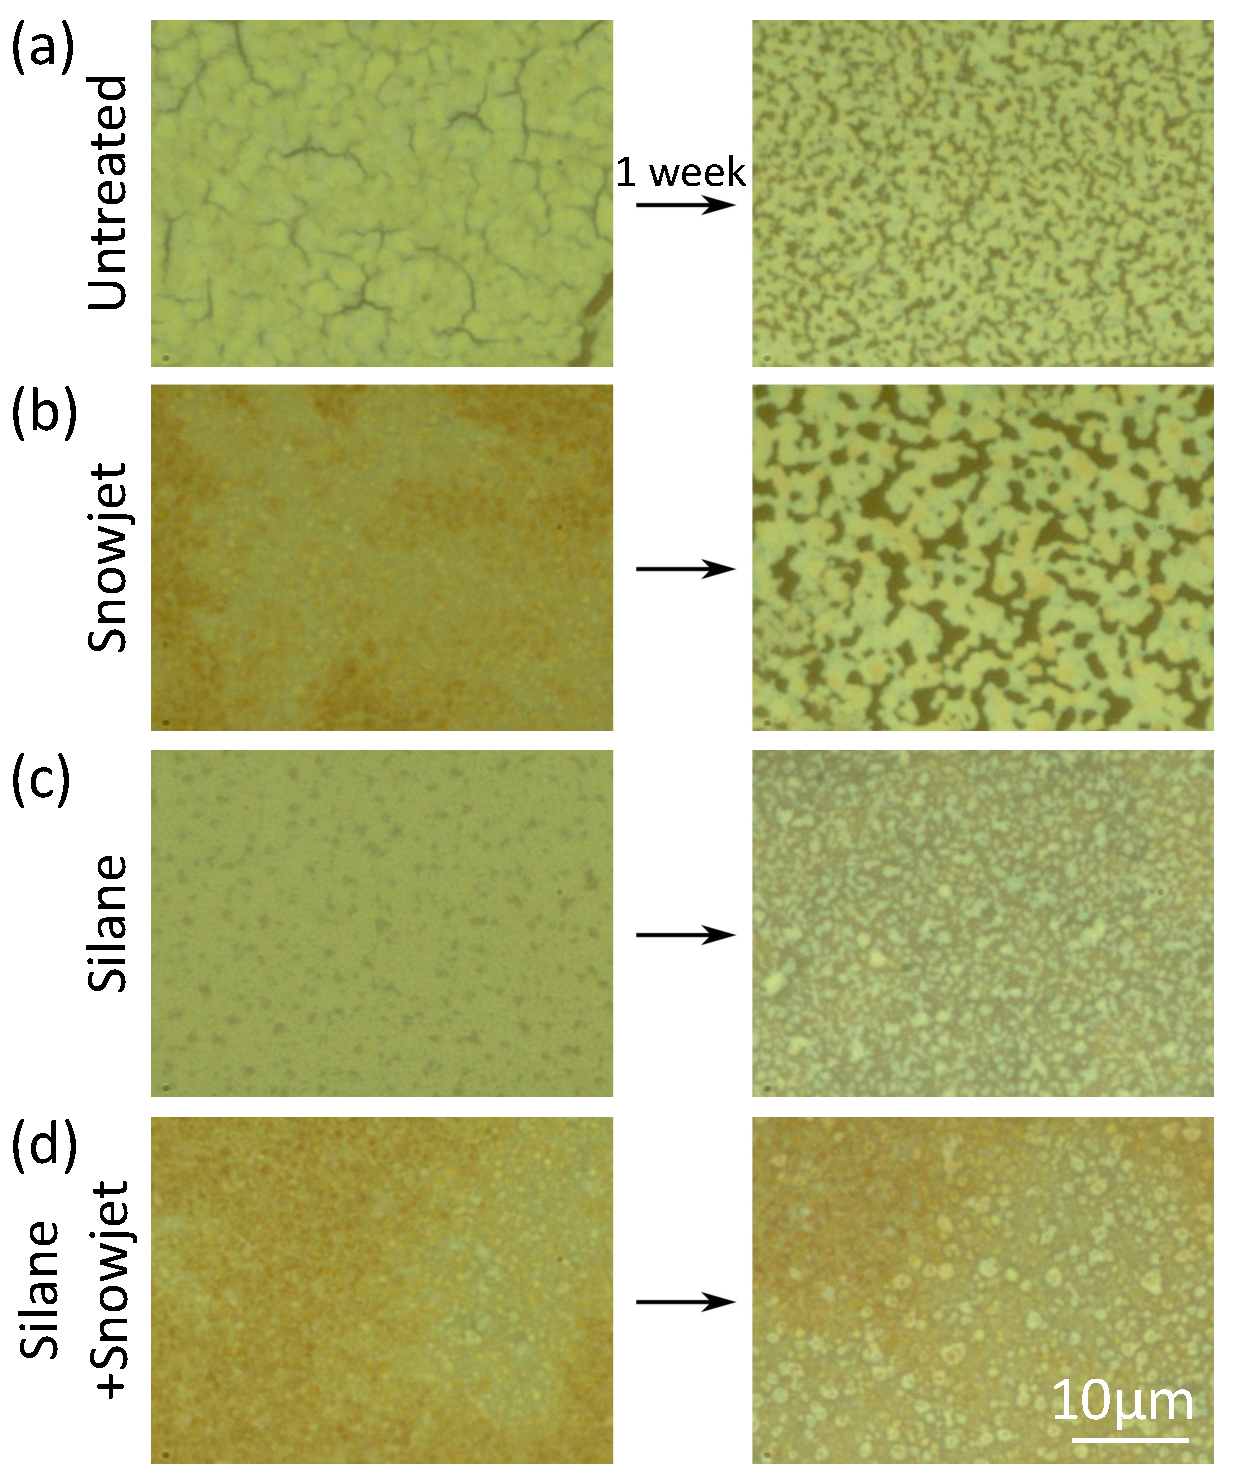
\includegraphics[width=0.65\textwidth]{Fig4}
\caption{Degradation of 2000\,rpm C$_{12}$PI thin films shown in $100\times$ magnification BF images. Images of the sample were taken as-made (left), and after one week in standard conditions (right).}
\label{4Fig4}
\end{figure}
\subsection{Sample degradation}
BF images at 100$\times$ magnification of 2000\,rpm C$_{12}$PI films as-made (left) and after one week in standard conditions (right) are shown in Fig.\,\ref{4Fig4}. All films show signs of dewetting or diffusion, highlighting the importance of placing C$_n$PI films in low humidity atmospheres, or capping with polymer layers to prevent sample degradation \cite{Pradeesh2009}. The images from Fig.\,\ref{4Fig1} and spectra from Secs.\,\ref{sec:4-2} and \ref{sec:4-3} are recorded within one day of film production.

\begin{figure}[h!] 
\centering    
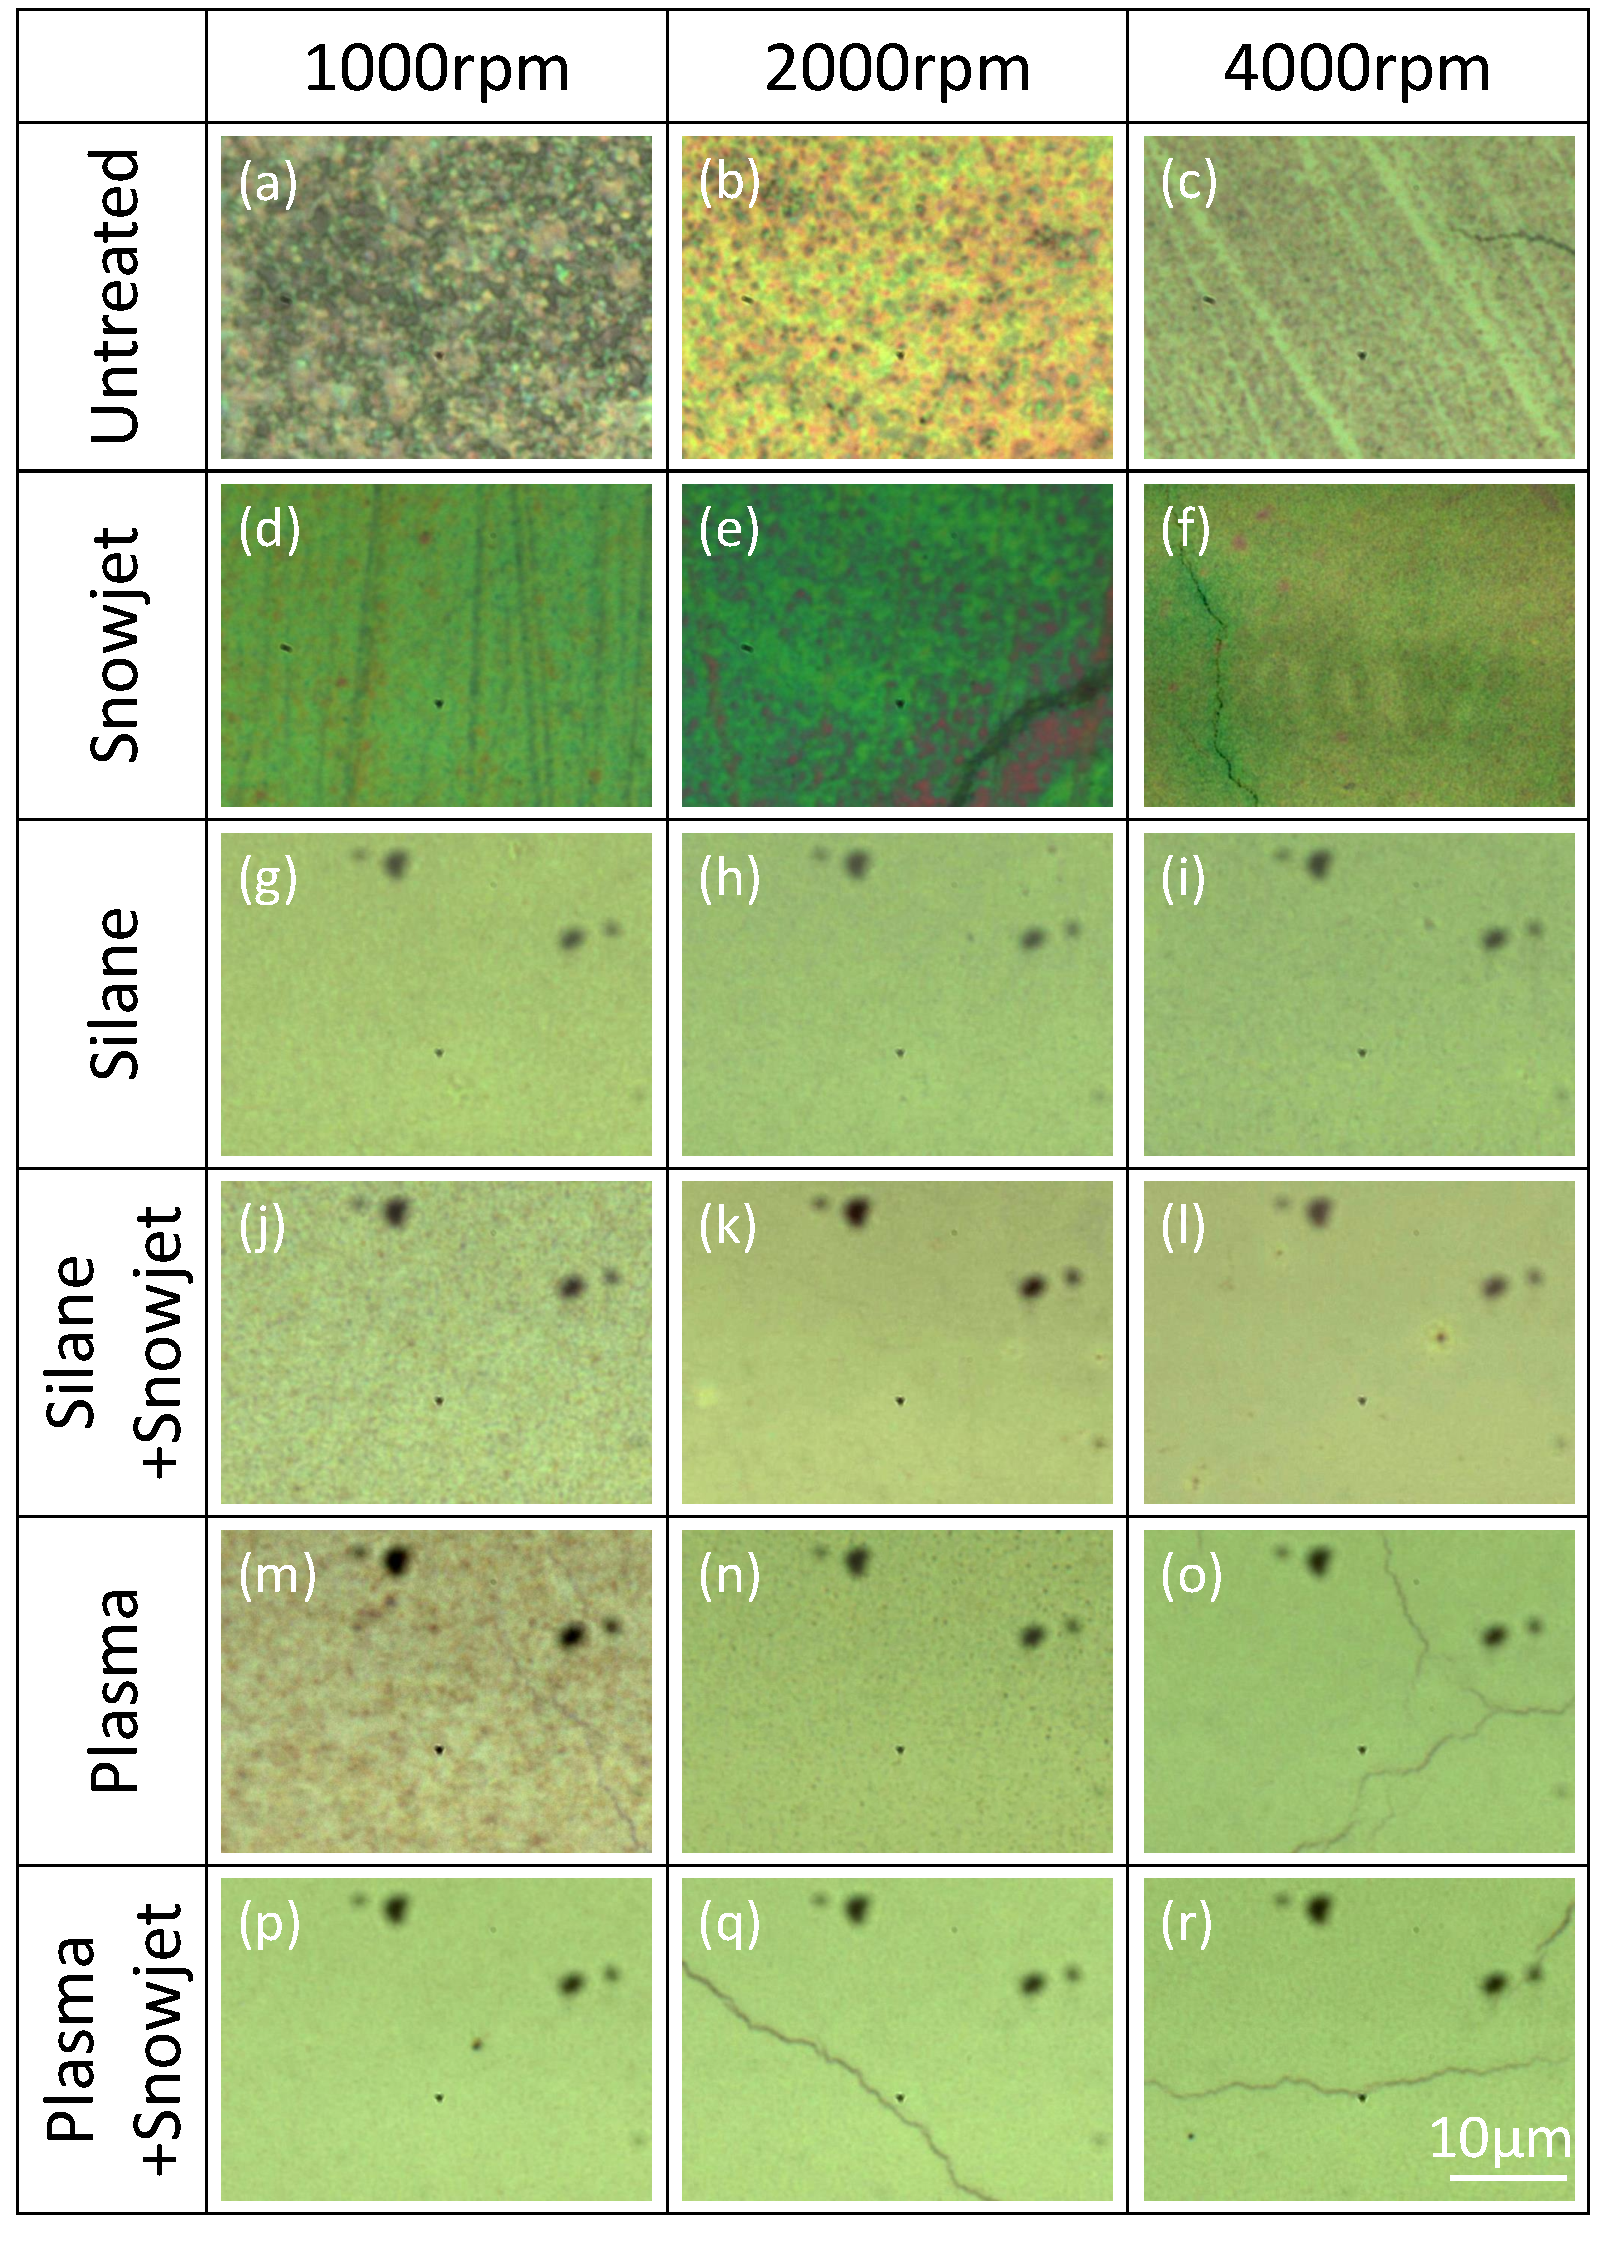
\includegraphics[width=0.9\textwidth]{Fig5}
\caption{BF images at 100$\times$ magnification of spin coated CHPI films on silica, with spin speed and substrate preparation as labelled. The black marks seen on (g-r) are due to dust particles on the microscope lens.}
\label{4Fig5}
\end{figure}
\section{CHPI thin films}
BF images of CHPI films at 100$\times$ magnification are shown in Fig.\,\ref{4Fig5}. No dewetting is observed with CHPI due to increased hydrophilicity of the organic molecule. Both snowjetting and high spin speeds improved the uniformity of samples [Figs.\,\ref{4Fig5}(a-f)], however the best films are produced with silanised substrates, regardless of spin speed [Figs.\,\ref{4Fig5}(g-l)]. A similar effect is seen for plasma etched substrates [Figs.\,\ref{4Fig5}(m-r)].

\subsection{Spin speed}
\label{sec:4-5}
\begin{figure}[h!] 
\centering    
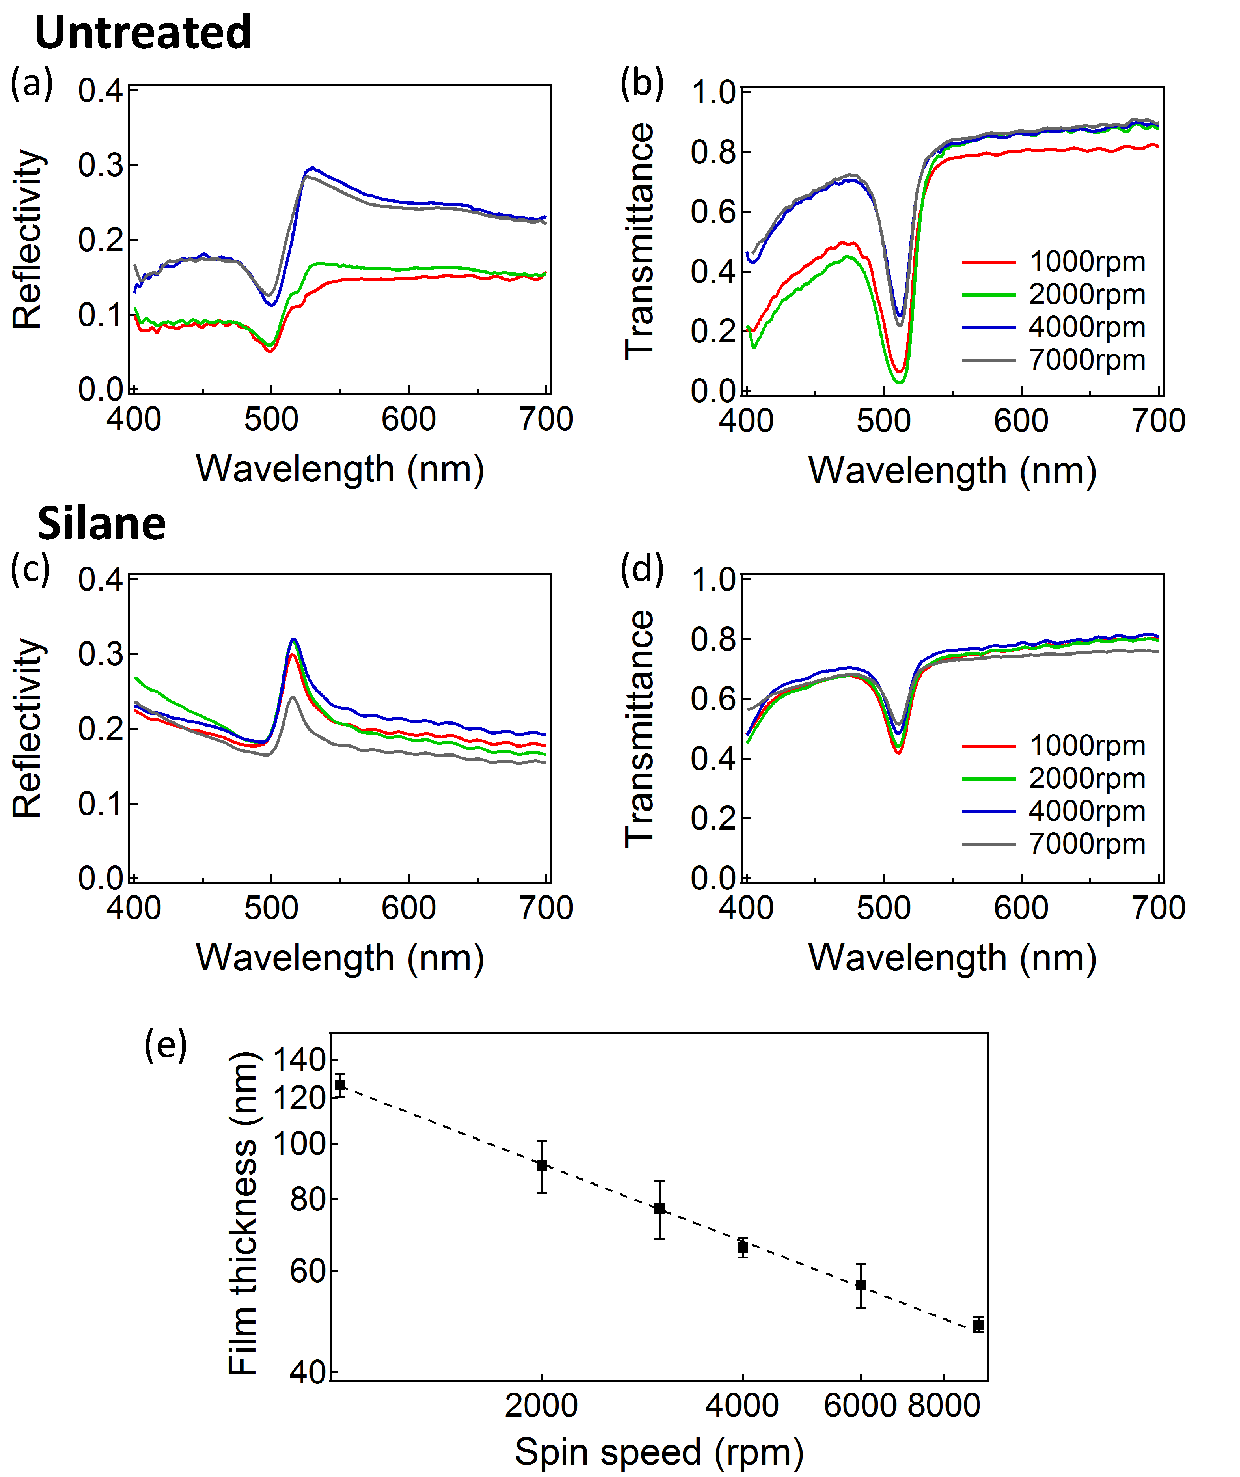
\includegraphics[width=\textwidth]{Fig6}
\caption{Reflection and transmission spectra for CHPI films prepared on (a,b) untreated and (c,d) silanised silica substrates. (e) Effect of spin speed on CHPI film thickness on untreated substrates for 30\,mg/ml solutions. Error bars provide the standard deviation from 10 different films, and the dashed line represents a fit to $a\omega^{-b}$, with $b=0.45\pm0.01$.}
\label{4Fig6}
\end{figure}
Optical spectra of CHPI films created on untreated or silanised substrates are shown in Fig.\,\ref{4Fig6}, with the exciton resonance at the expected wavelength of 506\,nm \cite{Pradeesh2009b}. For untreated substrates, noticeable differences in the spectra between 2000 and 4000\,rpm films are caused by a morphology change: at low spin speeds increased film roughness produces lower overall reflectivity, and the appearance of a higher energy exciton leads to an apparent increase in the linewidth of the transmission dip [Figs.\,\ref{4Fig6}(a,b)]. Extra features that broaden the resonance peak have been observed in thick perovskite films ($>120$\,nm) and are attributed to stacking faults, strain and structural misalignment in the structure \cite{VijayaPrakash2009}. In contrast, as expected from their BF images [Fig.\,\ref{4Fig5}(g-i)] the spectra for silanised substrates exhibit the same features at all spin speeds [Figs.\,\ref{4Fig6}(c,d)], the main difference being a change in the amplitude of the exciton resonance as a result of the film thickness. 

Film thickness measurements for around 10 films on untreated substrates are fitted to $a\omega^{-b}$ with $b=0.45\pm0.01$ [Fig.\,\ref{4Fig6}(e)], close to the $\omega^{-0.5}$ relationship predicted by theory. Although this discrepancy may be attributed to the somewhat simplified model, a larger source of error comes from AFM measurements of film thickness. Film scratches are made using razor blades, thus AFM measurements may differ the true film thickness. It can also be difficult to provide accurate values due to film/substrate roughness, or small gradients in the film thickness. These effects are hard to quantify and not represented in Fig.\,\ref{4Fig6}(e), where the error bars are calculated from statistical analysis of the data recorded.

\begin{figure}[] 
\centering    
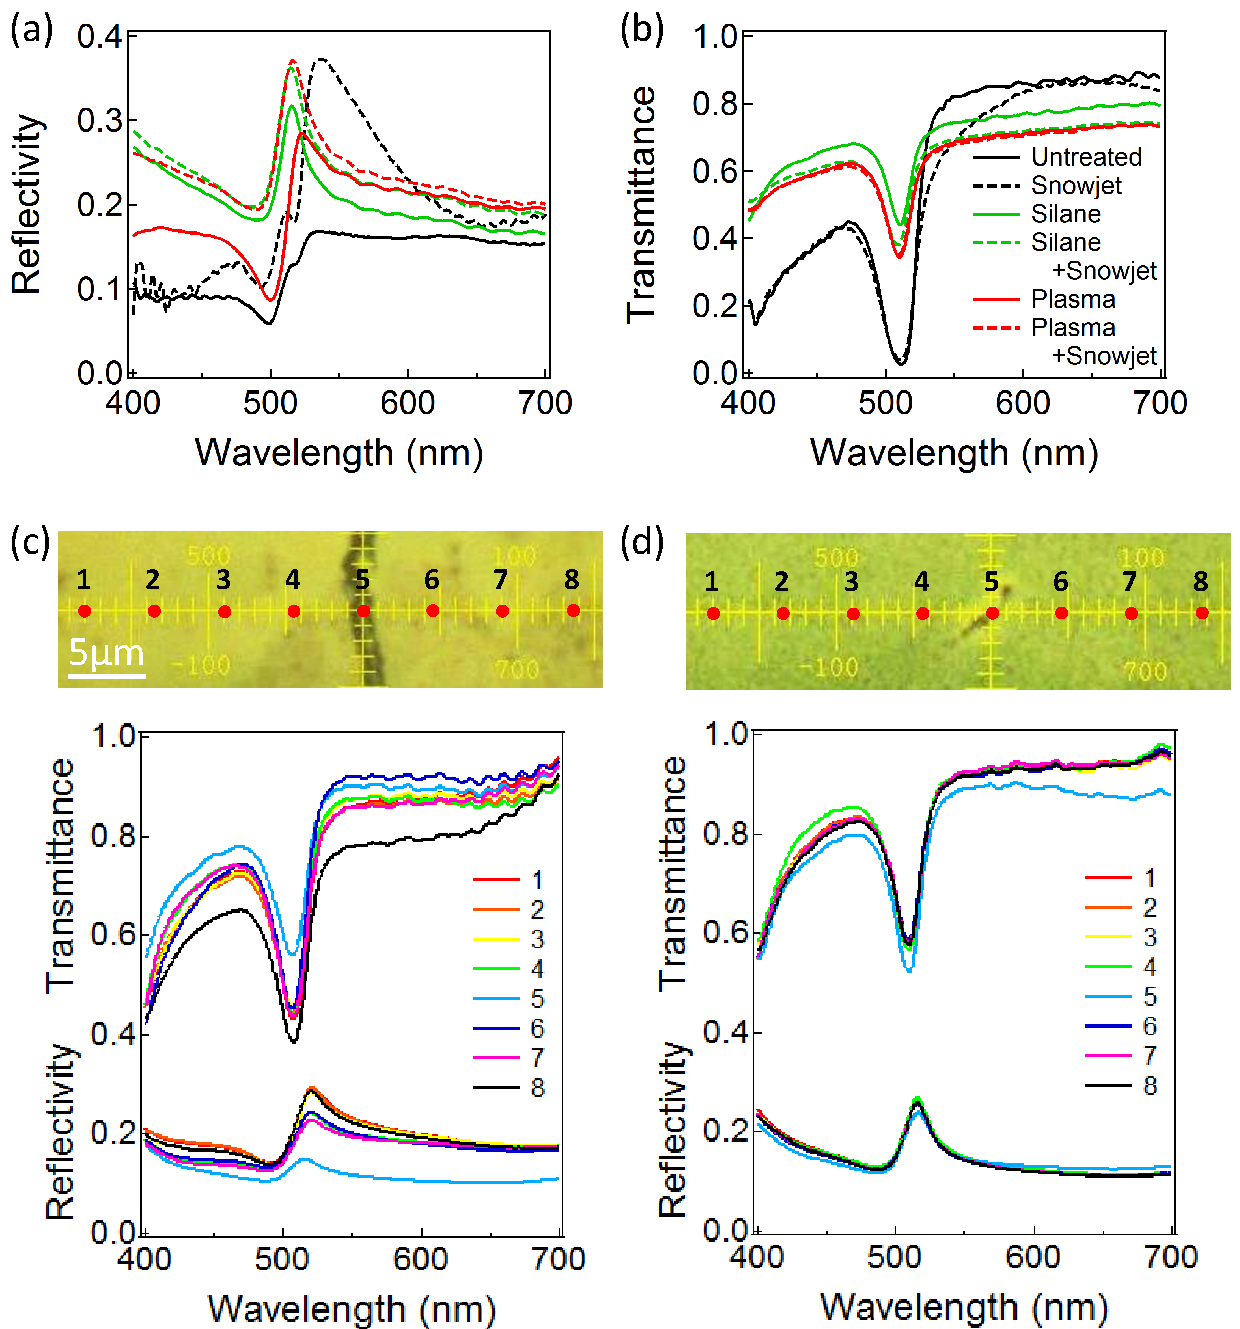
\includegraphics[width=\textwidth]{Fig7}
\caption{(a) Reflection and (b) transmission spectra (collected over areas with diameter $\approx 20\,$\textmu m) of 2000\,rpm CHPI films. Reflection and transmission spectra (diameter $\approx1\,$\textmu m) of 4000\,rpm CHPI films prepared on (c) untreated and (d) silanised and snowjetted silica substrates at the positions indicated on the images above.}
\label{4Fig7}
\end{figure}
\subsection{Substrate preparation}
Optical spectra of 2000\,rpm CHPI films made using a variety of substrate preparation techniques are shown in Fig.\,\ref{4Fig7}. The appearance of a second exciton due to structural misalignment [Sec.\,\ref{sec:4-5}] is seen for both untreated and snowjetted films. As indicated by their BF images [Fig.\,\ref{4Fig5}(h,k,n,q)], the spectra and morphologies of films made using other substrate preparations are very similar, and the uniformity is greatly improved by functionalisation of the substrate via silanisation or plasma etching. As an indication of the sample uniformity, line scans were made on 4000\,rpm films made using untreated [Fig.\,\ref{4Fig7}(c)], and silanised and snowjetted [Fig.\,\ref{4Fig7}(d)] substrates (signals collected over areas with diameter $\approx1\,$\textmu m). Cracks and discolourations can be seen in the case of the untreated substrate as a result of substrate non-uniformity [Fig.\,\ref{4Fig7}(c)], while the only defect seen for the silanised substrate comes from a piece of dust of the substrate [position 5 on Fig.\,\ref{4Fig7}(d)]. The near-identical spectra of all areas on the functionalised substrate is further proof of the film uniformity observed in BF images [Fig.\,\ref{4Fig7}(d)].

\begin{figure}[h!] 
\centering    
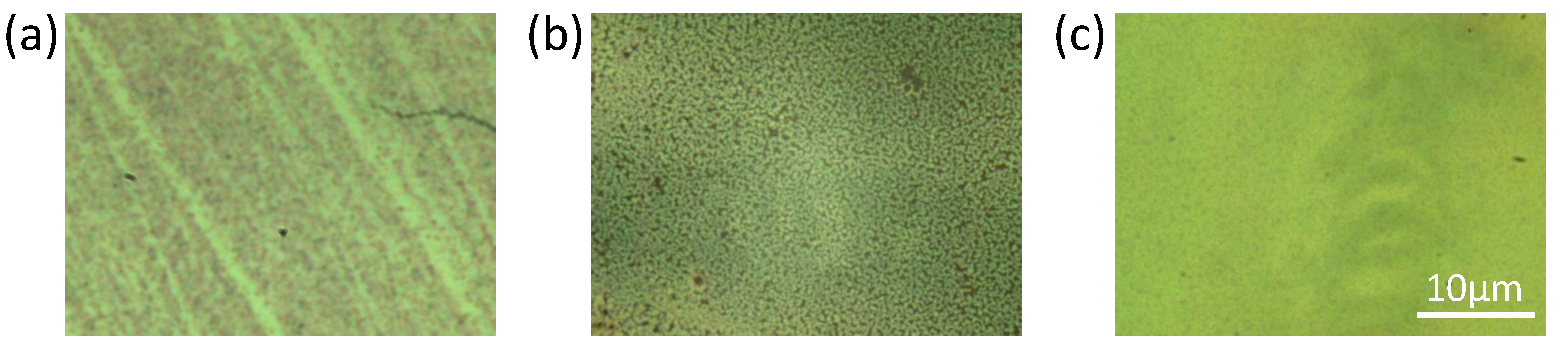
\includegraphics[width=\textwidth]{Fig8}
\caption{BF images at 100$\times$ magnification for 4000\,rpm CHPI films made on untreated substrates in (a) low humidity, (b) high humidity and (c) dehydrated spin coater atmospheres. (d) AFM measurements of above films.}
\label{4Fig8}
\end{figure}
\subsection{Humidity}
Hydrogen bonding between the organic and inorganic constituents is essential to assembly of the perovskite structure, therefore unwanted bonding or screening due to water molecules in the atmosphere can disrupt this process. A continuous CHPI film is formed at 4000\,rpm on an untreated substrate in a low humidity atmosphere [Fig.\,\ref{4Fig8}(a)], however the same spin coating conditions lead to dewetting at high humidity despite the hydrophilic organic group [Fig.\,\ref{4Fig8}(b)]. Ideally the spin coater should be desiccated as much as possible, and in order to achieve this the dehydration agent \ce{CaCl2} is placed inside the spin coater roughly one hour before film production. The spin coater is also pumped with \ce{N2} gas just before spinning, and the resulting film is very uniform even without the use of substrate functionalisation [Fig.\,\ref{4Fig8}(c)]. AFM measurements show that film roughness is reduced by a decrease in humidity as expected from BF images [Fig.\,\ref{4Fig8}(d)]. Films made in high humidity atmospheres have roughness on the order of the film thickness due to dewetting, while films made with CaCl have roughness $\sim5$\,nm.


\section{Conclusions}
Thin films of PbI perovskites with thickness $30-150$\,nm can be produced reliably using spin coating. Film morphology depends strongly on the organic molecule used in the perovskite, and dewetted films are produced for hydrophobic moieties. However film coverage and uniformity can be improved by using higher spin speeds, or substrate functionalisation techniques such as silanisation. Film thickness is controlled by the spin speed and initial solution concentration, and follows an $\omega^{-0.45}$ dependence, close to theoretical predictions. Formation of the perovskite structure can be disrupted by water in the atmosphere, and a dehydration agent should be placed in the spin coater to controllably produce a low humidity environment. The simplicity and adaptability of spin coating allows PbI perovskite thin films to be deposited on suitable substrates in order to create hybrid nanostructures.
%*****************************************************************************************
%*********************************** Fifth Chapter **************************************
%*****************************************************************************************

\chapter{Micromechanical exfoliation of lead iodide perovskites}

\graphicspath{{Chapter5/Figures/}}

\nomenclature[z-CHPI]{CHPI}{\ce{(C6H9C2H4NH3)2PbI4}}
\nomenclature[z-C12PI]{C12PI}{\ce{(C12H25NH3)2PbI4}}
\nomenclature[z-MWQ]{MQW}{Multiple quantum well}
\nomenclature[z-BF]{BF}{Bright field}
\nomenclature[z-DF]{DF}{Dark field}
\nomenclature[z-AFM]{AFM}{Atomic force microscope}
\nomenclature[z-SPP]{SPP}{Surface plasmon polariton}
\nomenclature[z-LSP]{LSP}{Localised surface plasmon}
\nomenclature[z-SEM]{SEM}{Scanning electron microscope}

\section{Introduction}
Uniform thin films of PbI perovskites can be created over large areas as a result of spin coating, however it is hard to achieve thicknesses $\lesssim30$\,nm and probe the properties of ultra-thin samples. For thinner samples a layer-by-layer deposition technique can be used \cite{Era2000, Matsui2002}. Micromechanical exfoliation is another way of achieving such samples: cleaving thicker crystals to separate the layers and form progressively thinner samples.

In recent years much attention has been paid to 2D layered compounds such as graphene or transition metal dichalcogenides. Due to weak van der Waals bonding, it is easy to cleave neighbouring layers and form ultra-thin samples \cite{Novoselov2004, Blake2007, Ni2007, Splendiani2010, Castellanos-Gomez2010, Tonndorf2013}. In these materials new optical and electronic properties emerge for mono- or few-layer regions, providing new avenues for material application. In this chapter we report micromechanical exfoliation of 2D PbI perovskites, and explore the few-layer behaviour of such systems via optical spectroscopy.

\section{Experimental methods}
A schematic of the preparation of exfoliated of PbI perovskites is shown in Fig.\,\ref{5Fig1}. Lead iodide (\ce{PbI2}) microcrystals are synthesized using a previously described solvothermal method, and intercalated using an 8\,mg/ml organic ammonium iodide/toluene solution to create hexagonal perovskite microcrystals $\sim\negmedspace30\,\mu$m in lateral size \cite{Saikumar2012}. The crystals were then heated at $50^{\circ}$C to completely remove the intercalation solution. We then use a micromechanical exfoliation technique to create thinner flakes, transferring the resulting samples onto an oxidized silicon (Si) wafer for further measurements. The thinnest regions are identified using optical microscopy, and then characterized with white light spectroscopy and atomic force microscopy (AFM).
\begin{figure}[ht] 
\centering    
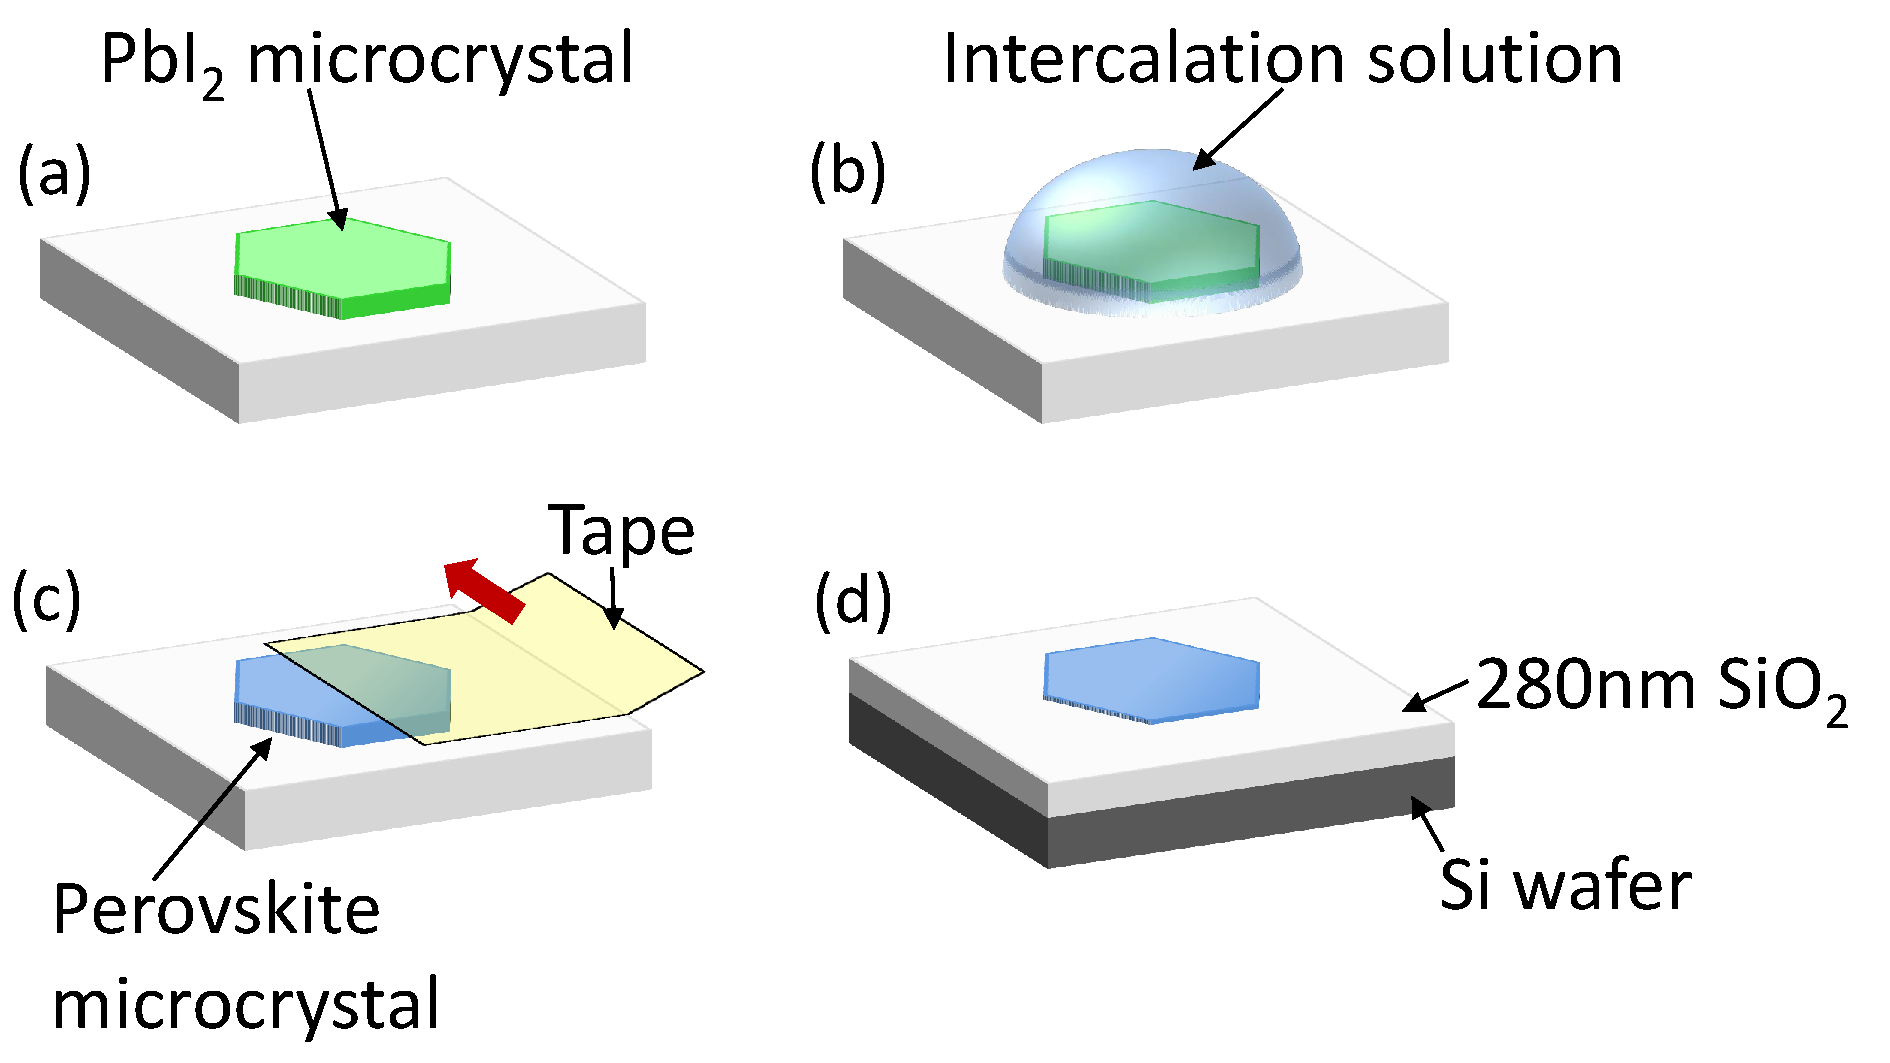
\includegraphics[width=0.8\textwidth]{Fig1}
\caption{Schematic of the preparation of exfoliated CHPI samples.}
\label{5Fig1}
\end{figure}

\section{Results}
BF images of intercalated CHPI and C12PI microcrystals at 20$\times$ magnification are shown in Fig.\,\ref{5Fig2}(a,b). Reflectivity spectra for such microcrystals shown an exciton resonance at $\sim500$nm indicating correct formation of the 2D structure, with Fabry-Perot fringing due to the thickness of the crystals (typically $\sim1\,\mu$m. The top surface of the crystals are rough as a result of etching by the intercalation solution, however as a result of the exfoliation process such surfaces should adhere to the tape and not be present in the transferred flakes for measurement. The exciton wavelength (grey dashed line) varies from the values from literature as it has been shown that a build up of strain in thick layer stacks can lead to structural distortions/rearrangements \cite{Saikumar2012, VijayaPrakash2009, Pradeesh2009b} thus changing the exciton energy. 

\begin{figure}[ht] 
\centering    
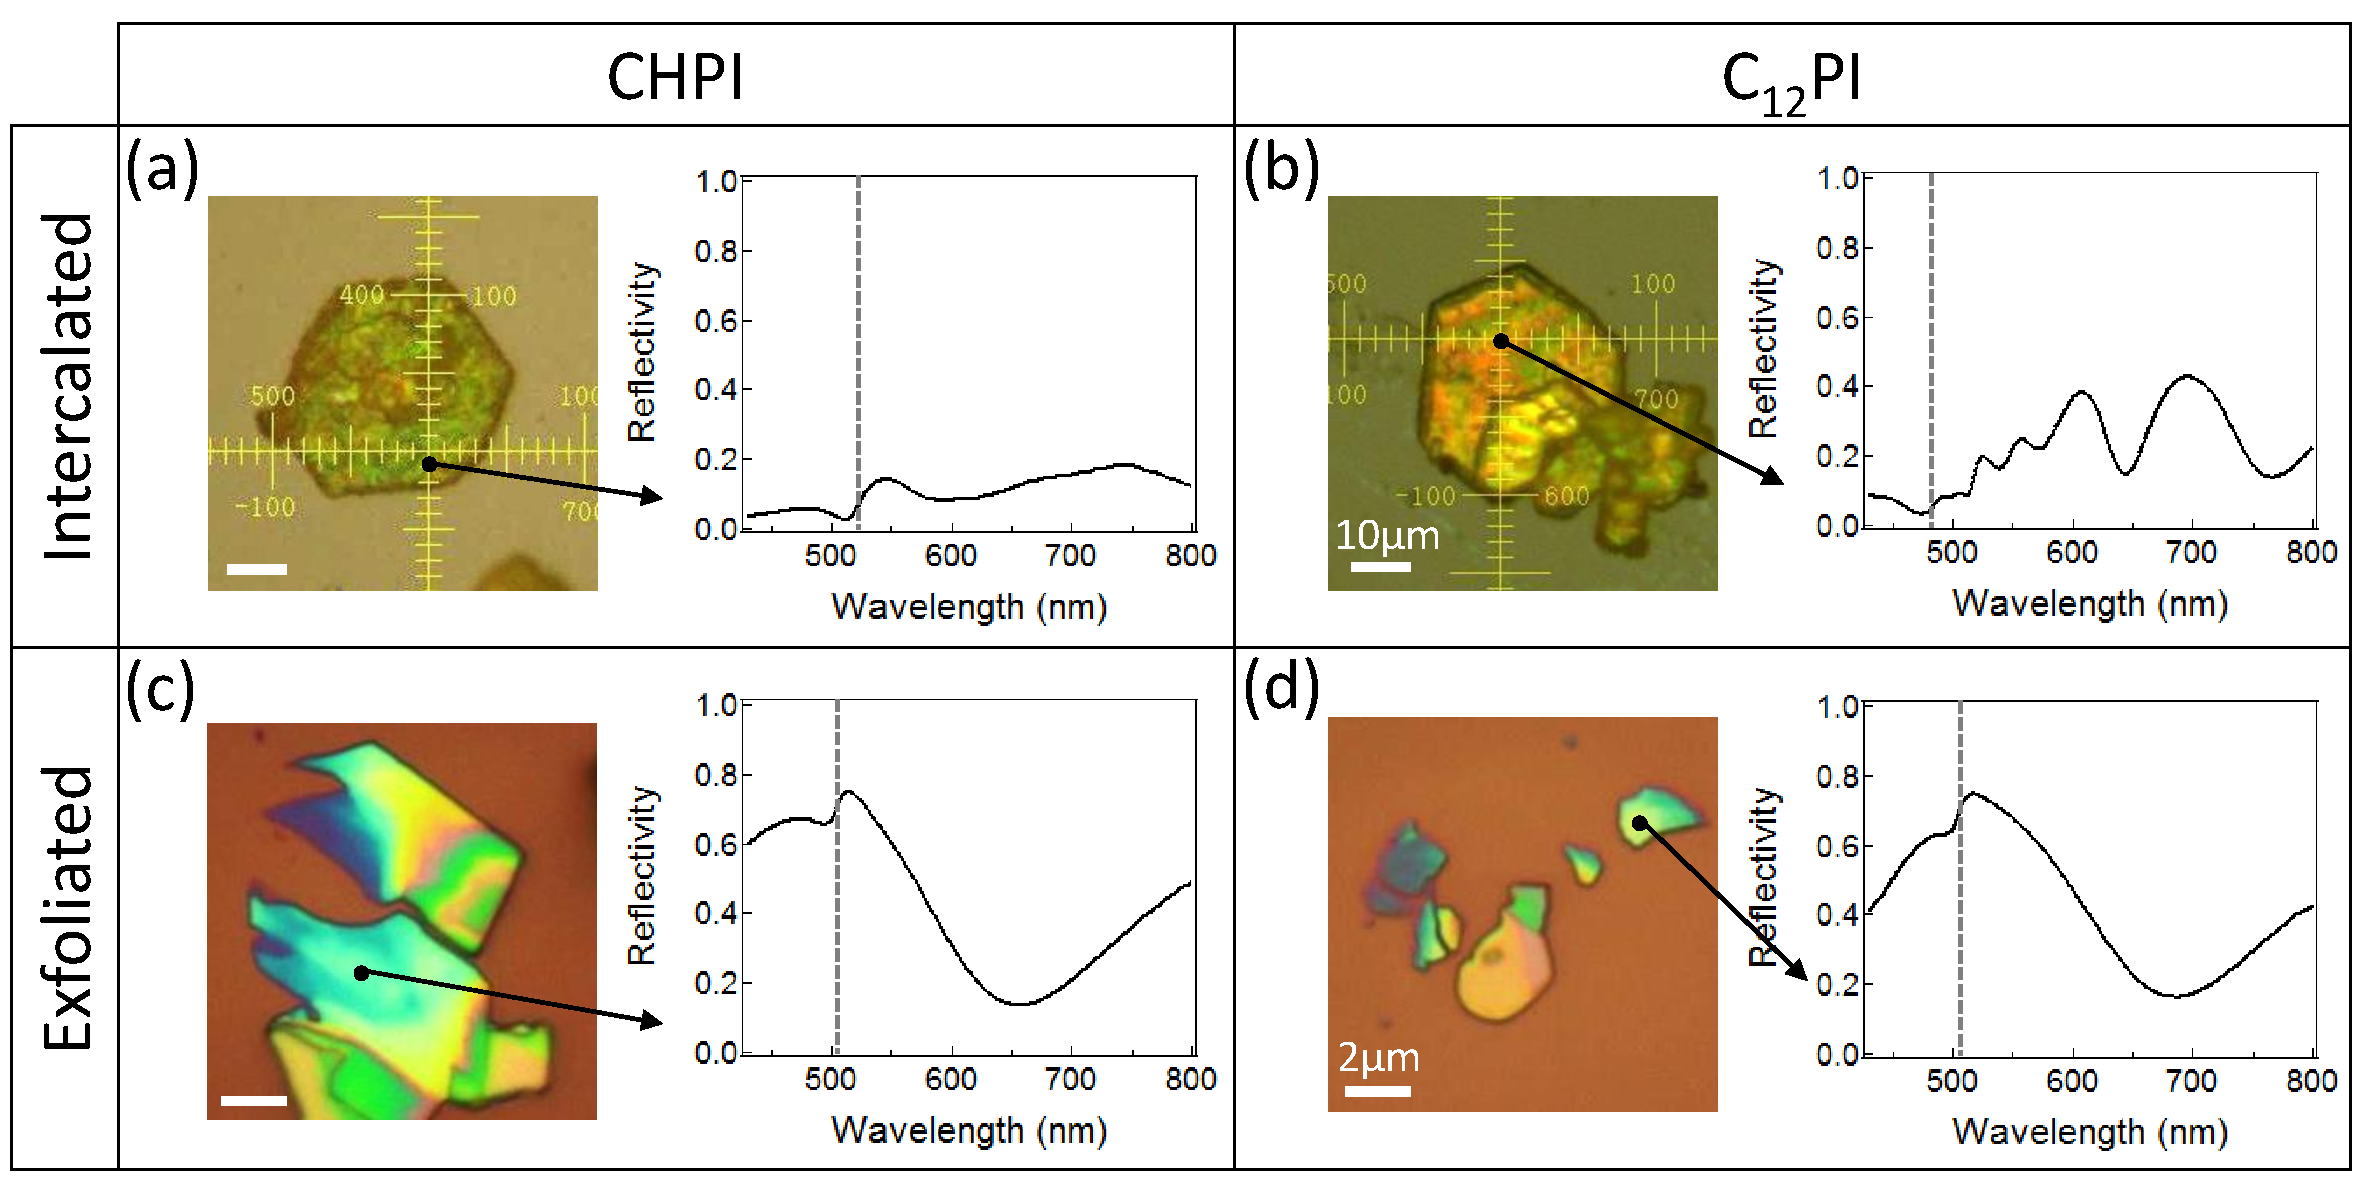
\includegraphics[width=\textwidth]{Fig2}
\caption[Intercalated and exfoliated perovskite microcrystals.]{Bright field images of intercalated (a) CHPI and (b) C12PI microcrystals on glass at 20$\times$ magnification, and exfoliated (c) CHPI and (d) C12PI flakes at 100$\times$ magnification. The reflectivity spectra of the areas indicated on the samples are also given. Grey dashed lines indicate the wavelength of the exciton resonance.}
\label{5Fig2}
\end{figure}
\subsection{Exfoliated CHPI microcrystals}

BF images of exfoliated flakes of CHPI and C12PI [Fig.\,\ref{5Fig2}(c,d)] are very similar. Although the crystals may fracture during the exfoliation process, we are able to obtain ultra-thin samples with lateral sizes of $\sim1-10\,\mu$m. The excitonic resonance is still seen in such samples, however due to the bistability of excitons in C12PI we use CHPI samples for further analysis.

\begin{figure}[ht]
\centering
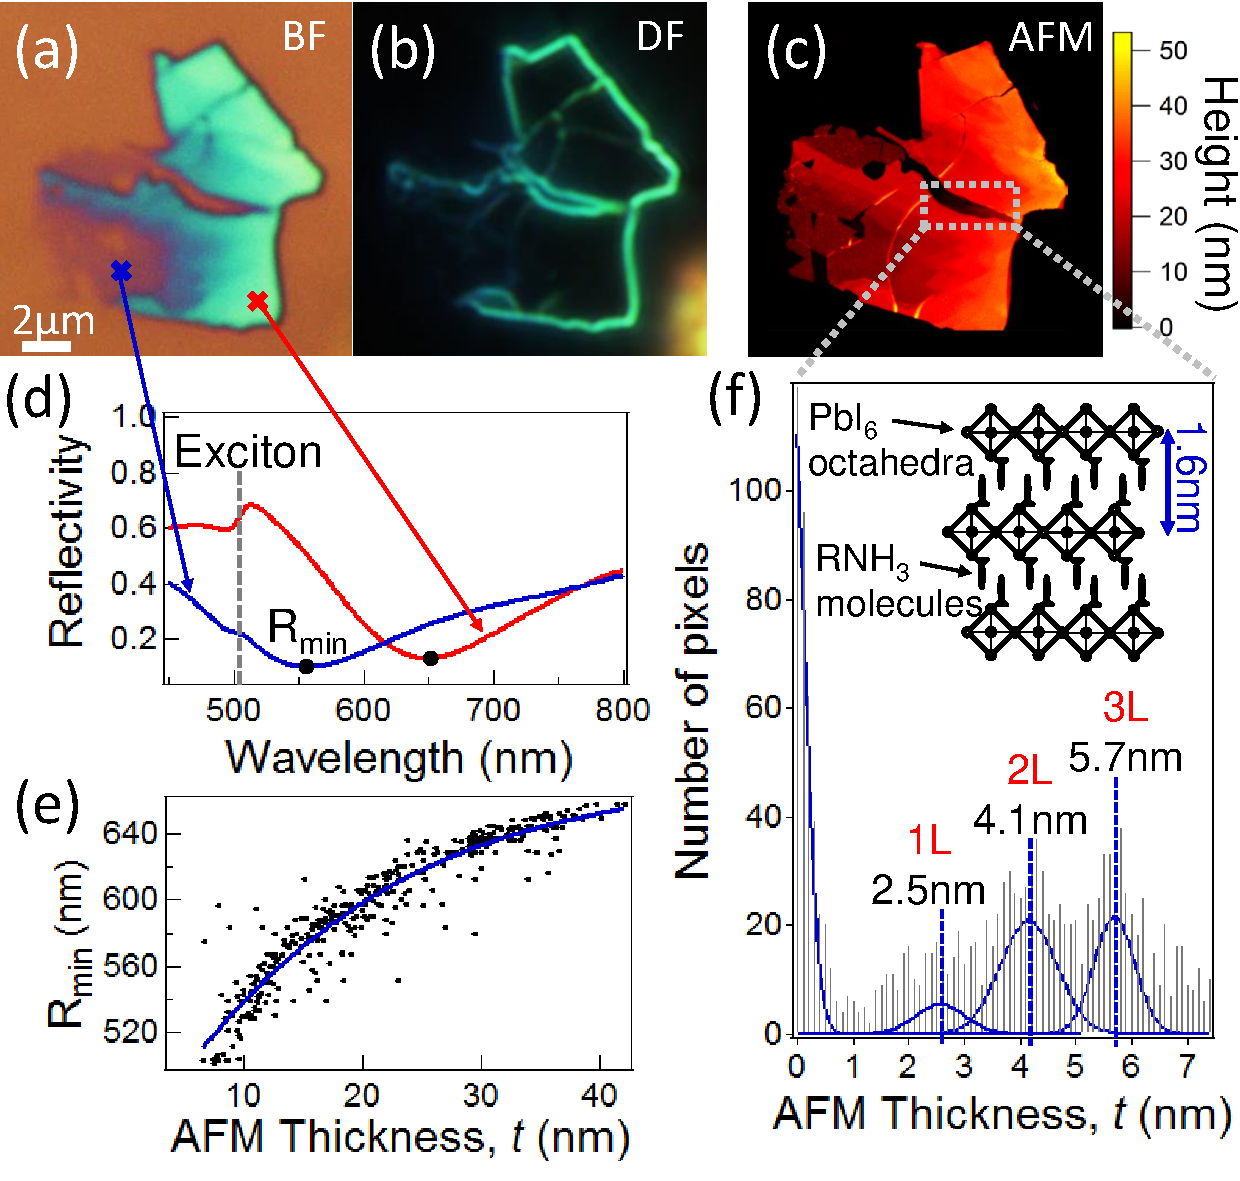
\includegraphics[width=0.8\textwidth]{Fig3}
\caption[Microscopy, spectroscopy and AFM measurements on exfoliated CHPI flakes.]{Images in 100$\times$ magnification using (a) bright and (b) dark field on an exfoliated CHPI flake; (c) AFM image of the same area. (d) Reflectivity spectra of two regions on the flake. The exciton wavelength is indicated by the dashed line. (e) Relationship between the measured reflectivity minimum (labelled as $\textnormal{R}_\textnormal{min}$ in (d)) and AFM thickness. (f) Histogram of heights measured in the boxed area of (c). Multipeak fitting to the data (blue lines) gives an interlayer spacing of 1.6\,nm. The inset shows the structure of 2D PbI perovskites.}
\label{5Fig3}
\end{figure}

BF and DF reflection images of a typical CHPI flake are shown at 100$\times$ magnification in Figs.\,\ref{5Fig3}(a,b) respectively. The DF scattering seen from the edges and grain boundaries of the sample is typical for such crystals. The reflectivity spectra for these exfoliated samples [Fig.\,\ref{5Fig3}(d)] consist of an excitonic Fano resonance at $\lambda_{ex}\negmedspace\approx\negmedspace504$\,nm superimposed on a background of Fabry-Perot fringes. These fringes correspond to the colour of the crystal seen in BF, and come from the path difference experienced by light double passing through the flake. The oxide layer on the substrate is designed to maximize optical contrast for very thin layers, and while optimized for graphene, this 280\,nm \ce{SiO2}/Si system also works well for CHPI. By using this spectral information in conjunction with AFM measurements [Fig.\,\ref{5Fig3}(e)], we can correlate the position of Fabry-Perot fringes with thickness $t$. Thus it is then possible to spectroscopically determine the thickness of CHPI flakes.

A histogram of AFM heights in the boxed area of Fig.\,\ref{5Fig3}(c) shows three predominant thicknesses, which can be fit to Gaussians separated by steps of 1.6\,nm [Fig.\,\ref{5Fig3}(f)]. This interlayer spacing agrees well with X-ray diffraction measurements, where the periodicity was found to be 1.7-1.8\,nm \cite{Billing2006b, Pradeesh2009a}. Due to the presence of molecules adsorbed on the surface of the substrate, the initial step of 2.5\,nm is likely due to a monolayer, allowing us to label the three peaks as 1-, 2-, and 3-layer regions.  

Spectroscopic measurements of flake thickness require detailed knowledge of the CHPI refractive index, which is not well known. Instead we extract the required information from reflectivity data using the transfer matrix formulation \cite{Born1999}. In the wavelength range of interest (460\,-\,750\,nm), the dielectric function $\epsilon$ of 2D PbI perovskites can be modelled as the sum of a constant background and two Lorentzian oscillators: the exciton ($ex$) and an additional charge transfer ($CT$) transition at $\sim\negmedspace400$\,nm \cite{VijayaPrakash2009, Fujisawa2004, Fujisawa2005, Fujisawa2007, Mitzi1999a, Zhang2010}. Hence
\begin{equation}
\centering
\epsilon = \epsilon_1+i\epsilon_2+\frac{A_{ex}}{\lambda_{ex}^2-\lambda^2+i\Gamma_{ex}\lambda}+\frac{A_{CT}}{\lambda_{CT}^2-\lambda^2+i\Gamma_{CT}\lambda} ,
\label{CHPI_model}
\end{equation}
where $\epsilon_1, \epsilon_2$ are the background terms, while $A_i$ is the amplitude, $\lambda_i$ the wavelength, and $\Gamma_i$ the linewidth of oscillator $i$. The refractive index ($\tilde{n} = \sqrt{\epsilon}$) can then be used in the multilayer transfer matrix to calculate the expected reflectivity. The $CT$ peak, due to the charge transfer between organic and inorganic layers, is particular sensitive to disorder and the local dielectric environment, and depends on the precise spin coating conditions when comparable thin films are produced \cite{VijayaPrakash2009}. 

\begin{figure}[ht]
\centering
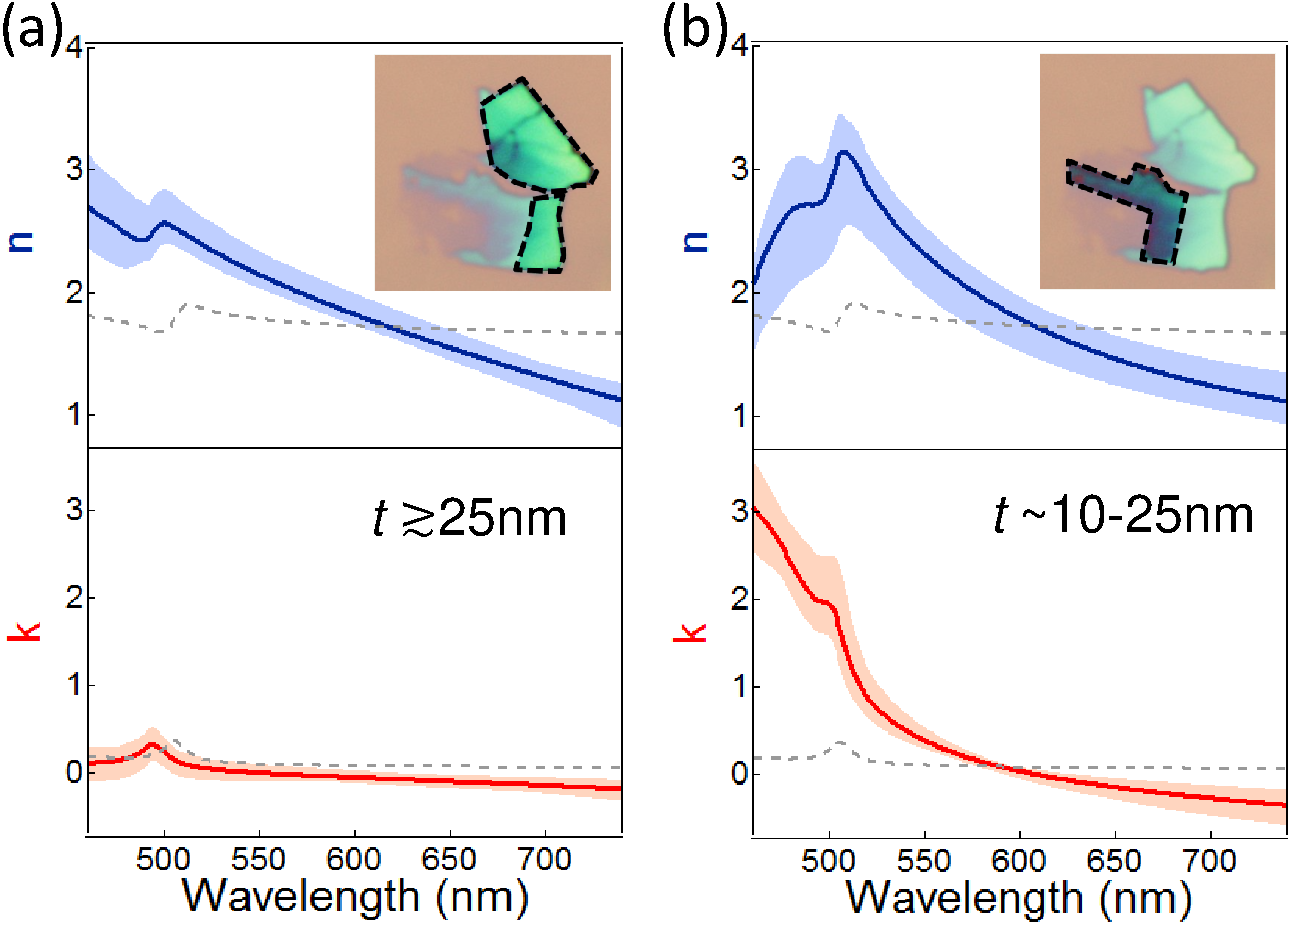
\includegraphics[width=0.8\textwidth]{Fig4}
\caption[Fitted complex refractive index of CHPI flakes.]{Fitted complex refractive index of CHPI flakes for more than 200 pixels. Two regimes are found: (a) low absorption, occurring at positions of high thickness ($t\negmedspace\gtrsim\negmedspace25$\,nm), and (b) high absorption, at lower thickness ($t\negmedspace\sim\negmedspace10\negmedspace-\negmedspace25$\,nm). The insets indicate typical areas where each regime is found. Shaded regions show the range of values extracted from the fit, and grey dotted lines represent the refractive index of a CHPI film ($t\negmedspace\sim\negmedspace60$\,nm) measured using ellipsometry.}
\label{5Fig4}
\end{figure}

The results of these refractive index fits for more than 200 spectra are shown in Fig.\,\ref{5Fig4}. The fitting works well for spectra that are not collected at the edges of the flake, therefore the thinnest areas are excluded. Within these regions, two main regimes of refractive index are observed. In both cases the background and exciton oscillator are relatively unchanged. For thicker areas of the sample ($t\negmedspace\gtrsim\negmedspace25$\,nm) a low-absorption regime is observed, where the $CT$ oscillator is mainly reflective. For thinner areas ($t\negmedspace\sim\negmedspace10\negmedspace-\negmedspace25$\,nm) a high-absorption regime is seen, where the $CT$ oscillator redshifts and becomes more optically active. As discussed below, the thickness range encompassed by the absorbing regime is correlated with a region of structural reconfiguration. This leads to a change in the energy states of the hybrid perovskite, and modifies the charge transfer between neighbouring organic and inorganic sheets. For comparison, the refractive index of a $t\negmedspace\sim\negmedspace60$\,nm film extracted from ellipsometry (grey dashed line) is also shown in Fig.\,\ref{5Fig4}. The film absorption ($k$) is closer to that of thicker flake areas, with a reduced contribution from the $CT$ oscillator in the refractive index. X-ray diffraction shows that while distinct layers are formed during spin coating, there is greater structural disorder in each layer when compared with intercalated \ce{PbI2} microcrystals \cite{Saikumar2012}. This interface mismatch can be responsible for a large range of charge transfer environments, leading to the reduced strength of the $CT$ resonance that we observe here.

\begin{figure}[ht]
\centering
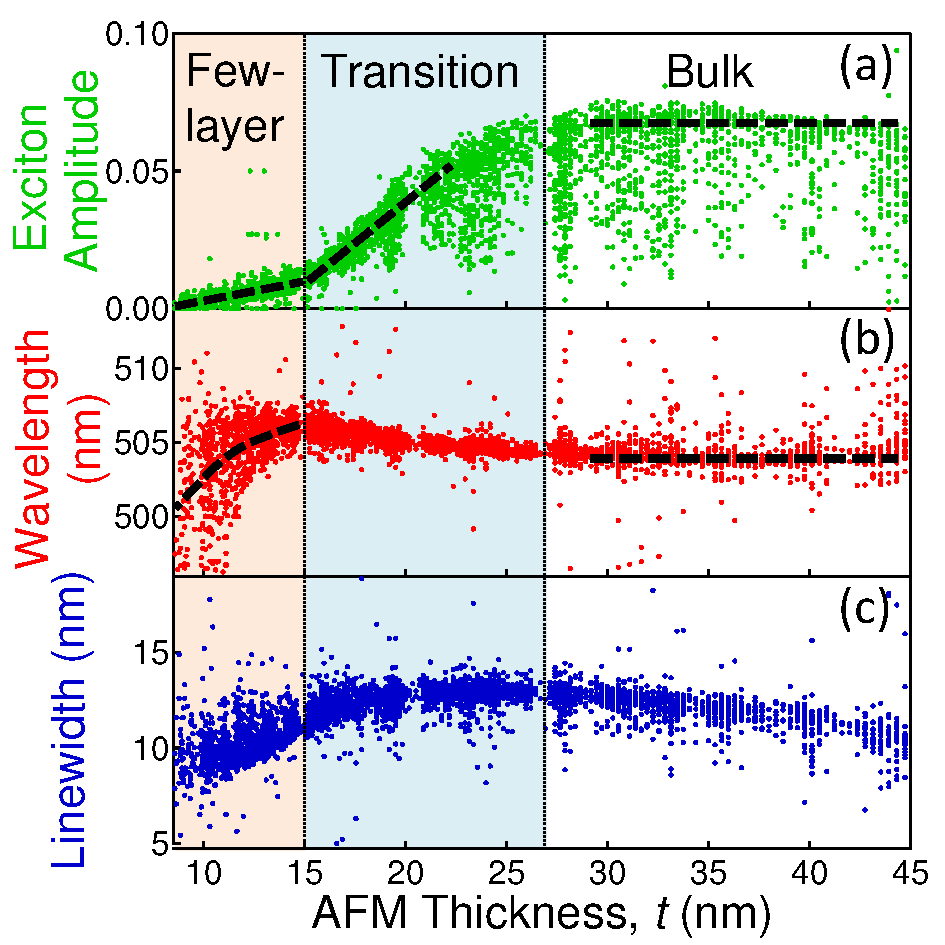
\includegraphics[width=0.8\textwidth]{Fig5}
\caption[Change in exciton properties of CHPI with flake thickness.]{Fitted exciton (a) amplitude, (b) wavelength, and (c) linewidth from reflectivity spectra (see Eq.\,\ref{R_fit}). Dashed lines are guides for the eye.}
\label{5Fig5}
\end{figure}

In reflectivity the exciton produces a Fano lineshape due to interference between its narrow resonance and the continuum background. On account of this complication, we extract information about exciton properties by describing $\Delta R = R_{\textnormal{CHPI}} - R_{substrate}$ as
\begin{equation}
\centering
\Delta R = R_{bkg} + A\frac{(\lambda - \lambda_{ex} + q\gamma)^2}{(\lambda - \lambda_{ex})^2 + \gamma^2} , 
\label{R_fit}
\end{equation}
where $R_{bkg}$ represents the continuum background with Fabry-Perot fringing; $A$, $\lambda_{ex}$ and $\gamma$ are the amplitude, wavelength, and linewidth of the exciton respectively, and the parameter $q$ describes the asymmetric shape of the Fano resonance. The results of the fit are shown in Fig.\,\ref{5Fig5} for positions across many flakes with different thicknesses. $A$, $\lambda_{ex}$ and $\gamma$ are equivalent to the corresponding terms in Eq.\,\ref{CHPI_model}, while $q$ represents the interference between the exciton, CT and background terms. Near the vicinity of the exciton the effects of the CT and background are not distinguished, therefore Eq.\,\ref{R_fit} allows us to focus exclusive on the exciton components, while Eq.\,\ref{CHPI_model} gives us the overall refractive index. Since the perovskite resembles a multilayer system, we find the exciton amplitude initially scales linearly with the number of layers as expected, before saturating at $t\negmedspace\approx\negmedspace27$\,nm (15 layers). The large variability of amplitudes at high thickness arises predominantly from spectra taken at edges of flakes. Linear extrapolation of our data indicates the exciton amplitude will drop to zero at $t\negmedspace\sim\negmedspace7$\,nm (3 layers). However layer-by-layer assembly of perovskite films has shown that linear increases in the exciton intensity occur only after the fourth layer, while two monolayers are required to observe room temperature exciton behaviour \cite{Matsui2002}. 

From Fig.\,\ref{5Fig5}, we identify 3 regions of interest. Firstly the `bulk' region ($t\negmedspace\gtrsim\negmedspace27$\,nm), where the exciton wavelength remains roughly constant; secondly the transition region ($t\negmedspace\sim\negmedspace15\negmedspace-\negmedspace27$\,nm), where the wavelength begins to redshift, while the linewidth reaches a maximum; and finally the few-layer region, where the wavelength blueshifts below the bulk limit, along with a decrease in the linewidth. This data helps us understand the changes happening at a structural level: disorder causes inhomogeneous broadening of the exciton resonance \cite{Baranovskii1993, Andreani1998, Kuznetsova2010}, while the exciton energy is directly related to the angle between \ce{PbI6} octahedra in the inorganic layers \cite{Pradeesh2009}. In `bulk' CHPI, the exciton has a wavelength of 504\,nm and a spectral width of $\approx\negmedspace10$\,nm. Close to the thickness transition region, the system is seen to become more disordered as the PbI sheets rearrange, becoming flatter and more strained. Finally at small $t$, the few-layer regime reveals how the layers relax and crumple again to reach the lowest energy configuration. Extrapolation of the fitted exciton wavelength to monolayer thickness (3\,nm) leads to a wavelength of $\sim\negmedspace495$\,nm, comparable to the value of $\sim\negmedspace490$\,nm reported for \ce{PbI2} thin films \cite{Iwasaki1978, Goto1987}. We were unable to spectroscopically probe areas with $t\negmedspace<\negmedspace8$\,nm (4 layers) as they lie on the edges of flakes, and are around 100\,nm in size. Since the lateral resolution of reflectivity measurements is $1\,\mu$m, these spectra are averaged with the much bigger signals from thicker areas. In order to achieve more sizeable monolayer regions, large-area samples are desirable for exfoliation, for instance using solution-grown single crystals. Exfoliating onto flexible polymer substrates may also improve our capability for attaining large monolayer regions as this can reduce fracture of crystals. However our measurements clearly show that these organic-inorganic hybrid perovskites change their electronic properties as the thickness is reduced, and this is connected to changes in the strain, disorder and layer structure.

\section{Conclusions}
In conclusion, we report the exfoliation of 2D organic-inorganic perovskites. Monolayers are observed, and the interlayer distance was found to be 1.6\,nm. As with other 2D materials, the thinnest regions (\textless8 layers) behave differently from the bulk material due to the influence of strain on the layer structure. We note however that the active excitonic layers are already electronically isolated in these hybrids, so changes in the band structure as observed in dichalcogenide systems are not expected. Instead, the effects seen are due to the re-organisation of organic molecules around the inorganic sheets. This suggests that pre-organisation of the intercalating molecules is key to controlling material structure at the monolayer scale, which may be accessible through chemical growth rather than exfoliation. This work suggests the potential to construct optoelectronic devices for monolayers of these hybrid materials, offering new routes to emission. 

%*****************************************************************************************
%*********************************** Sixth Chapter **************************************
%*****************************************************************************************

\chapter{Perovskite-coated metal islands}

\graphicspath{{Chapter6/Figures/}}

The interactions between localised surface plasmons (LSPs) and the materials in their vicinity can be utilised for a host of applications. For example, sensitivity of the resonance frequency to the local dielectric function can be exploited in sensing devices \cite{Jensen2000, Xu2004, Malinsky2001, Royer1987}, while the large field enhancements caused by electron oscillations can be used to increase Raman signals \cite{Cade2009, Olson2001, Talley2005} or emission rates \cite{Toftegaard2011, Cho2010, Reboud2013, Blanco2004}. LSP resonances of noble metal nanoparticles can be tuned across the visible spectrum via their geometries, so the fabrication of metal island nanostructures are often adjusted to suit the application.

In this Chapter the creation of Au/Ag nano-islands overcoated with a perovskite layer is described. Such systems are then used to understand light-matter coupling between excitons and LSPs, with a view to creating new quasiparticles via strong coupling.

\section{Metal island films}
Thin film morphology depends on interactions between the film and substrate atoms (i.\,e.\,the diffusion of metal atoms on substrate surface), as well as external conditions such as deposition rate, substrate temperature and subsequent annealing steps \cite{Kaiser2002}. Deposition via evaporation is a heterogeneous nucleation process, and requires high vapour pressure. Various growth modes are possible, but for noble metal films deposited on silica the metal-metal interactions are stronger than metal-substrate interactions, therefore islands are formed on the substrate \cite{Kaiser2002}. With increased deposition time islands can coalesce, either preserving the existing grain boundaries or forming a continuous structure \cite{Sennett1950,Gupta2002}.

Such metal island films (MIFs) are essentially nanoparticle arrays: if the islands are well separated (separation $l \gtrsim\,	$island diameter $d$) then there is no optical coupling between the particle resonances and we expect to see a single LSP resonance in optical spectra. The resonance wavelength of these arrays depend on the island geometry, and can be controlled by the thickness of the deposited film \cite{Walter2006, Sennett1950, Gupta2002, Gadenne2002, Lee1992}. As with nanoparticles we can model islands as dipoles embedded in a medium with dielectric function $\epsilon_d$ to predict the resonance wavelength, with care taken to include the effects of the substrate \cite{Yamaguchi1960, Yamaguchi1972, Yamaguchi1973, Doremus1966}.

\subsection{Experimental methods}
Silica substrates are prepared as described in Sec.\,\ref{sec:glass}. Metal deposition is performed using an Edwards resistance evaporator, under pressure $\sim4\times10^{-6}$\,mbar with deposition rate $\sim0.5$\,\AA/s. The substrates are not heated, and the deposited film thickness $t$ is determined by a 6\,MHz quartz crystal microbalance. To avoid oxidation, Ag samples are placed in a nitrogen purge dessication cabinet within 15\,minutes of fabrication, and only removed for further processing/characterisation. Annealed Au and Ag MIFs are made by heating the samples at $200^{\circ}$C for 24\,hours in vacuum. In order to create the CHPI overcoating, a CHPI/THF solution is spin coated onto the nanostructured films under a dehydrated atmosphere (layer thickness $\sim100$\,nm). The samples are then characterised using AFM, SEM and white light microscopy. During optical measurements 400 unpolarised reflection ($R$) and transmission ($T$) spectra are taken over a 0.5$\times$0.5mm$^{2}$ area and averaged to produce the data shown. Due to sample uniformity, this data is representative of the entire sample, and the absorption $A = 1 - R - T$ as scattering from these samples is less than 1\%.

\begin{figure}[h!] 
\centering    
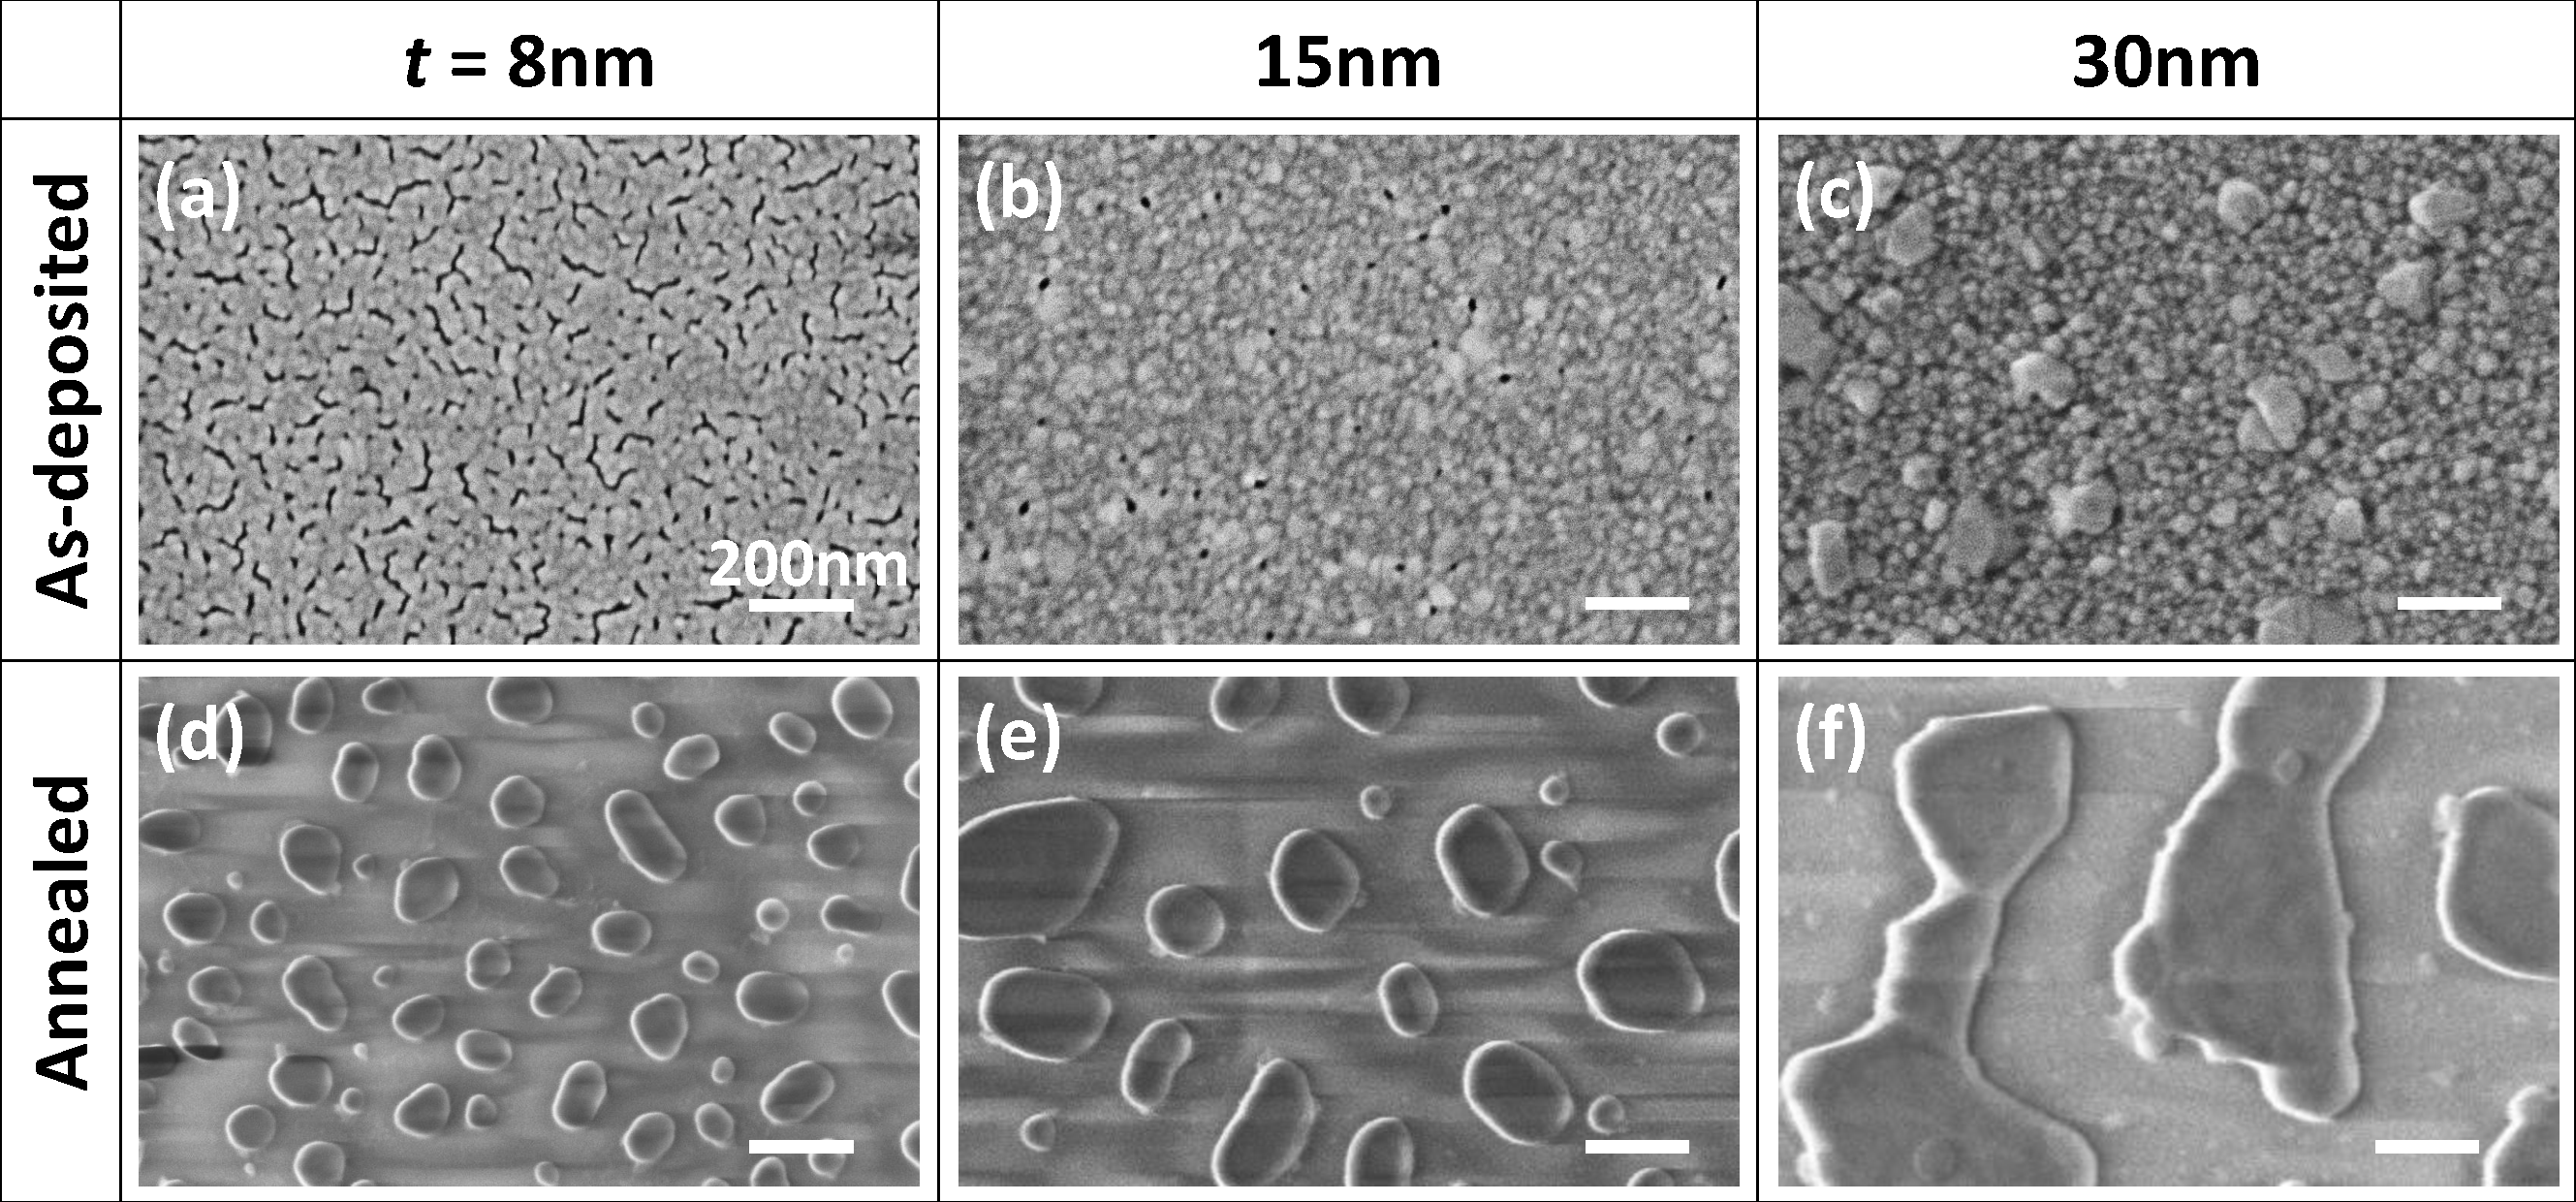
\includegraphics[width=\textwidth]{Fig1}
\caption{SEM images of (a-c) as-deposited and (d-f) annealed Au metal island films. The initial deposited film thickness $t$ is labelled.}
\label{6Fig1}
\end{figure}
\subsection{Au metal island films}

SEM images of evaporated Au films on silica show the formation of a rough but continuous film for $t=30$\,nm [Fig.\,\ref{6Fig1}(c)]. As $t$ decreases dewetting is observed as a result of weak Au-substrate interactions [Figs.\,\ref{6Fig1}(a,b)]. During annealing, Au atoms diffuse and form distinct islands [Figs.\,\ref{6Fig1}(d-f)]. With decreasing $t$ the islands become more closely spaced and ellipsoidal, smaller in both lateral size $d$ and height $h$ [Fig.\,\ref{6Fig2}]. For $t=8$\,nm we observe islands with $d \sim 50-100$\,nm, $h\sim70$\,nm, and separation $l \sim 100-200$\,nm. The decrease in island size is seen optically in 100$\times$ magnification DF reflection images, where scattering from the islands due to LSP resonances is broadband for $t=30$\,nm, but becomes progressively redder as the film thickness and island size decrease [Fig.\,\ref{6Fig2}]. 
\begin{figure}[h!] 
\centering    
\includegraphics[width=0.85\textwidth]{Fig2}
\caption{AFM profiles of annealed Au metal island films. The deposited film thickness $t$ is labelled. Insets show 100$\times$ magnification DF images of the samples.}
\label{6Fig2}
\end{figure}

Fig.\,\ref{6Fig3} shows the absorption spectra for $t=8$\,nm as-deposited and annealed Au MIFs. We observe a resonance $\lambda_{dep} = 570$\,nm in the absorption of the as-deposited film, however this is due to grains in the film and therefore has a large linewidth $\Gamma_{dep} = 245$\,nm. In the annealed film we observe a resonance $\lambda_{anneal} = 550$\,nm with linewidth $\Gamma_{anneal} = 50$\,nm due to island LSPs.

\begin{figure}[h!] 
\centering    
\includegraphics[width=\textwidth]{Fig3}
\caption{BF images at 100$\times$ magnification for CHPI films on (a) silica, (b) $t=8$\,nm as-deposited and (c) $t=8$\,nm annealed Au metal island films. (d) Average absorption spectra for 400 pixels over $0.5\times0.5$\,mm$^2$. The exciton wavelength is marked by the dashed line, and LSP resonances by arrows. The (annealed) Au MIF spectra are offset for clarity.}
\label{6Fig3}
\end{figure}
\subsection{CHPI-coated Au metal island films}

BF reflection images at 100$\times$ magnification show the formation of CHPI on silica [Fig.\,\ref{6Fig3}(a)] and $t=8$\,nm as-deposited and annealed Au MIFs [green areas in Figs.\,\ref{6Fig3}(b,c)]. The exciton resonance $\lambda_{ex} = 505$\,nm is observed for all three films, confirming formation of the MQW structure despite some roughness and dewetting on Au substrates. We observe a redshift in the LSP resonance as a result of the CHPI coating ($\lambda_{anneal} = 550$\,nm $\rightarrow 735$\,nm), with a considerable increase in the linewidth due to the non-uniform CHPI coverage ($\Gamma_{anneal} = 50$\,nm $\rightarrow 200$\,nm). However the excitons in CHPI are completely unaffected by the presence Au islands as the two oscillations are far off-resonance, so the exciton peak remains at the same wavelength and linewidth. The overall magnitude of the absorption across the entire visible range has increased as a result of absorption by the metal film.
%CHPI+annealed Au LSP linewidth ~500nm+?

\begin{figure}[h!] 
\centering    
\includegraphics[width=\textwidth]{Fig4}
\caption{SEM images of (a-c) as-deposited and (d-f) annealed Ag metal island films. The initial deposited film thickness $t$ is labelled. Dark areas/streaks in (a, d, e) are due to charging of the sample.}
\label{6Fig4}
\end{figure}
\subsection{Ag metal island films}

The morphology of evaporated Ag films on silica are similar to Au: rough films lead to dewetting with decreasing $t$, as well as formation of MIFs when the as-deposited films are annealed [Fig.\,\ref{6Fig4}]. However the Ag-substrate interactions are stronger as annealing does not cause island separation for $t=30$\,nm films, only an increase in grain size. Annealed $t=8$\,nm Ag MIFs consist of ellipsoidal islands with $d \sim40-100$\,nm, $h\sim80$\,nm, and $l\sim50-150$\,nm [Fig.\,\ref{6Fig5}]. DF images at $100\times$ magnification also show a change from broadband white scattering to green as $t$ decreases [Fig.\,\ref{6Fig5}]. 

\begin{figure}[h!] 
\centering    
\includegraphics[width=0.85\textwidth]{Fig5}
\caption{AFM profiles of annealed Ag metal island films. The deposited film thickness $t$ is labelled. Insets show 100$\times$ magnification DF images of the samples.}
\label{6Fig5}
\end{figure}

As seen in the SEM images, as-deposited Ag films are essentially continuous with some dewetting if $t>8$\,nm. Thus absorption spectra are similar to that of bulk Ag films, with an increase in absorption up to the band gap $\sim300$\,nm [Fig\,\ref{6Fig6}(a)]. However resonances can be observed for lower $t$, particularly $t=2$\,nm ($\lambda_{dep} = 560$\,nm, $\Gamma_{dep} = 175$\,nm), indicating formation of islands even without annealing [see also Sec.\,\ref{sec:AgonCHPI}]. 

After annealing, LSP resonances of Ag islands dominate the absorption spectra [Fig.\,\ref{6Fig6}(b)]. Although the positions of the absorption peaks do not change significantly with $t$, there is a clear decrease in the linewidth of the $t=2$\,nm film compared to the others [Fig.\,\ref{6Fig6}(c)]. The relative stability of the LSP wavelength suggests the average island size does not change with $t$. However we may have a larger range of island shape/size for thicker films, leading to a superposition of many resonance wavelengths and higher order LSP modes, and an apparent increase in the LSP linewidth.
\begin{figure}[h!] 
\centering    
\includegraphics[width=\textwidth]{Fig6}
\caption{Average absorption spectra for 400 pixels over $0.5\times0.5$mm$^2$ for (a) as-deposited and (b) annealed Ag metal island films with the thickness $t$. (c) Absorption peak position and linewidth for the spectra in (b).}
\label{6Fig6}
\end{figure}

\subsection{CHPI-coated Ag metal island films}
\label{sec:CHPI_AgMIF}
\begin{figure}[h!] 
\centering    
\includegraphics[width=\textwidth]{Fig7}
\caption{BF images at 100$\times$ magnification for CHPI films on (a) silica, (b) $t=8$\,nm as-deposited and (c) $t=8$\,nm annealed Ag metal island films. (d) Average absorption spectra for 400 pixels over $0.5\times0.5$mm$^2$. The exciton wavelength of the CHPI film on silica is marked by the dashed line. The (annealed) Ag MIF spectra are offset for clarity.}
\label{6Fig7}
\end{figure}
CHPI-coated Ag films behave similarly for $t\leq8$\,nm, so here we use $t=8$\,nm as an example. BF images at 100$\times$ magnification show very little difference between CHPI films on silica, as-deposited or annealed Ag MIFs [Fig.\,\ref{6Fig7}(a-c)], although some non-uniformity is observed in the case of the annealed Ag MIF. From the optical spectra in Fig.\,\ref{6Fig7}(d), we can see that as-deposited Ag MIFs cause little change to the exciton wavelength and linewidth, although the absorption has increased by 33\%. However for annealed Ag MIF the island LSP shifts to $\sim550$\,nm due to the CHPI coating and overlaps with the exciton resonance. Thus we see weak coupling in the form of a blueshift in the exciton wavelength by 5\,nm  ($\lambda_{ex}=500$\,nm), as well as an enhancement of the exciton absorption peak by 42\%. Coupling-induced enhancement of semiconductor absorption due to LSP field enhancements is a well-known phenomenon \cite{Balci2014, Alemu2014, Zheng2011, Xu2013, Spinelli2012}, however we were unable to observe modification of the exciton wavefunction via strong coupling as the LSP is not fully resonant with the exciton.

\subsection{Ag islands on CHPI films}
\label{sec:AgonCHPI}

Instead of coating Ag MIF films with CHPI, we also fabricated samples of Ag islands deposited on a CHPI film on silica. Since the CHPI organic molecules undergo a melting transition $\sim$80$^{\circ}$C \cite{Barman2003}, we thermally evaporate only 2\,nm of Ag to prevent degradation of the CHPI film due to heat. The AFM profile of a 2\,nm as-deposited Ag MIF on silica [Fig.\,\ref{6Fig8}(b)] shows the formation of separated metal islands, with $d\sim30$\,nm and $h\sim6$\,nm, %WN
however this measured height is likely due to the AFM tip not reaching the substrate due to its finite radius ($\approx 100$\,nm). %end
The AFM profile of an Ag MIF on CHPI is dominated by surface roughness of the CHPI film ($\sim$5\,nm, \textit{cf} Fig.\,\ref{6Fig8}(a)), however some high frequency noise on the order of $d$ can also be seen. The lack of distinct MIF features suggests Ag islands may be partially embedded in the CHPI film. However the thermal evaporation of Ag has not significantly damaged the CHPI film as a strong exciton peak can still be seen in absorption spectra [Fig.\,\ref{6Fig8}(d)]. In the same way as Sec.\,\ref{sec:CHPI_AgMIF}, the Ag island LSPs have again weakly coupled to excitons, causing a blueshift of 4\,nm but an increase in absorption of only 9\% in this case [Fig.\,\ref{6Fig8}(d)].
\begin{figure}[h!] 
\centering    
\includegraphics[width=\textwidth]{Fig8}
\caption{AFM profiles of (a) CHPI film on silica, (b) $t=2$\,nm evaporated Ag film on silica, and (c) $t=2$\,nm evaporated Ag film on CHPI. Insets show 100$\times$ magnification BF images of the samples. (d) Average absorption spectra for 400 pixels over $0.5\times0.5$mm$^2$. The exciton wavelength of the CHPI film on silica is marked by the dashed line. The Ag MIF spectrum is offset for clarity.}
\label{6Fig8}
\end{figure}

\section{Nanosphere lithography (NL)}
Nanosphere lithography involves the evaporation of metals through closely-packed 2D arrays of nano-/microparticles followed by removal of the spheres, leaving behind an array of metal islands on the substrate \cite{Haynes2001}. NL island array geometry depends on the diameter of spheres $D$. For a colloidal monolayer, the island diameter is $0.223D$, while the inter-island separation is $0.58D$ \cite{Hulteen1995}. The interstices between spheres lead to formation of triangular islands, however for small $D$ the islands can become more spherical \cite{Hulteen1999}. Array geometry can also be controlled by the metal evaporation angle \cite{Haynes2002}.

Much like MIFs, these triangular NL islands produce an LSP peak in optical spectra that depends on the size/shape of islands as well as the dielectric environment \cite{Jensen2000}, and can be modelled as an array of dipoles \cite{Malinsky2001, Jensen1999}. However nanosphere lithography provides better control of the island geometry due to the lithography mask, and should provide a sharper LSP resonance compared to MIFs.

\begin{figure}[h!] 
\centering    
\includegraphics[width=0.8\textwidth]{Fig9}
\caption{(a) Schematic of the creation of PS colloidal monolayers on a water droplets. SEM of (b) colloidal monolayer formed after the evaporation of water, and (c) triangular islands formed after the evaporation of Au and removal of colloids.}
\label{6Fig9}
\end{figure}
\subsection{Experimental methods}
We use $D=460$\,nm polystyrene (PS) microspheres from Sigma Aldrich to create the colloidal monolayer. The 10\,vol\% microsphere solution in water is diluted in a 1:1 mix with ethanol (absolute). Silica substrates are cleaned as described in Sec.\,\ref{sec:glass} then plasma etched for 1\,minute to create a hydrophilic surface. The substrates are placed at a $10^{\circ}$\,angle before a deionised water droplet is applied to cover the silica surface. A 2\,wt\% solution of sodium dodecylsulphate in water ($<0.5\,$\textmu l) is applied to the water surface, where the amphiphilic molecules act to reduce the surface charge on PS microspheres. A pipette is used to spread PS microspheres onto the droplet surface [Fig.\,\ref{6Fig9}(a)], and the water is allowed to evaporate under standard conditions. 50\,nm of Au is then deposited on the samples using an electron-beam evaporator system under pressure $\sim5\times10^{-6}$\,Torr at a rate of 1\AA/s. The PS microspheres are dissolved by placing the sample in a solution of dichloromethane for 30\,minutes, then sonicating the solution for 5\,minutes. Finally, a CHPI/THF solution is spin coated onto the island samples under a dehydrated atmosphere. Optical characterisation is performed by taking 400 scans over a $50\times50\,$\textmu m$^{2}$ region, then averaged to produce the spectra shown. 

\subsection{Au NL islands}
Closely-packed 2D arrays of PS microspheres are formed using this technique [Fig.\,\ref{6Fig9}(b)], and the ordering is best at contact lines of the solution. After the removal of PS, triangular islands are left behind on the silica substrate [Fig.\,\ref{6Fig9}(c)] with $d\sim90$\,nm. We can see from Fig.\,\ref{6Fig9}(c) that even in the best areas we do not find uniformly well-separated triangular islands. Due to small variations in the microsphere packing bow-tie shaped islands can form, and lines of Au are found at domain boundaries. However in the absorption spectra of such island samples [Fig.\,\ref{6Fig10}] we do observe an LSP resonance at 590\,nm with a linewidth of 80\,nm, comparable to MIF spectra.

\subsection{CHPI-coated Au NL islands}
Similar to CHPI-coated Au MIFs, strong exciton peaks in the absorption spectra of CHPI-coated Au NL islands indicate formation of the MQW structure. The exciton wavelength is unaffected by the Au ($\lambda_{ex} = 505$\,nm). As before, the LSP resonance redshifts due to the CHPI coating, and the linewidth broadens to $\sim$150\,nm. We observe a systematic increase of the LSP redshift as a result of increasing spin speed, and attribute this to more complete CHPI encapsulation of the Au islands as a result of larger forces at high spin speeds.
\begin{figure}[h!] 
\centering    
\includegraphics[width=0.7\textwidth]{Fig10}
\caption{Average absorption spectra for 400 pixels over $50\times50\,$\textmu m$^2$ of CHPI-coated Au nanosphere lithography islands. Arrows indicate the positions of LSP resonances, and the dashed line indicates the exciton wavelength. The spectra are offset for clarity.}
\label{6Fig10}
\end{figure}

\section{Conclusions}
Evaporation of noble metals can be %WN
used %end
to create ellipsoidal nanoparticles on a silica substrate. These metal island films behave like a nanoparticle array, and show distinct LSP resonances that can be tuned via deposition parameters. In the case of perovskite-coated Au islands the LSPs are far off-resonance with excitons, and the dielectric coating causes a redshift of the LSP peak with no effect on excitons. In the case of perovskite-coated Ag islands, LSPs weakly couple to excitons and cause a blueshift in the exciton resonance of 5\,nm, as well as an increase in exciton absorption by $\sim40$\% due to the electric field enhancement. Such enhancement has been investigated and is of particular interest for the design of solar cells \cite{Alemu2014, Zheng2011, Xu2013, Spinelli2012}.

The linewidth of the LSP resonance may be a barrier to strong coupling between plasmons and excitons in perovskite-coated nanostructures. The large variation in shape and size of metal particles in MIFs is an issue, however from our experiments the more controllable island geometries created using nanosphere lithography do not show a marked improvement in LSP linewidth. Chemically created metallic NPs, which are often pre-screened for size, may provide an avenue for future exploration, however a method of controllably assembling a dense array of well-separated NPs from solution will need to be investigated.
%*****************************************************************************************
%*********************************** Seventh Chapter **************************************
%*****************************************************************************************

\chapter{Perovskite-coated gratings}

\graphicspath{{Chapter7/Figures/}}

Despite their structural simplicity, 1D grating samples can sustain many electromagnetic modes, from diffractive interference to more localised and waveguided modes. In plasmonic gratings we can distinguish between such `photonic' gratings modes and the `plasmonic' modes that involve interactions with excited surface plasmon polaritons (SPPs), as described in Sec.\,\ref{sec:plasmonicgratings}. The dispersion and efficiency of grating modes in optical spectra depend on the coupling with incoming/outgoing photons, and is very sensitive to factors such as the polarisation of light, changes in geometry and the refractive index of any coating materials.

In this Chapter the optical behaviour of perovskite-coated 1D gratings is explored. Firstly CHPI-coated dielectric gratings are used to investigate the interactions between excitons and photonic grating modes, secondly coated non-plasmonic metallic gratings made from Ti introduce electrons to the system. Finally CHPI- and PS-coated Ag gratings are used to understand the coupling between excitons and SPPs. 

\section{Experimental methods}
\begin{figure}[h!] 
\centering    
\includegraphics[width=\textwidth]{Fig1}
\caption[(a) Fabrication and (b,c) setup of optical measurements on dielectric-coated metal gratings.]{(a) Fabrication of dielectric-coated metal grating. (b) Setup of angle-dependent reflectivity measurements. (c) Relationship between the polarisation of incoming light (black arrow) and azimuthal angle $\phi$ of the grating orientation. Red/blue arrows indicate the direction of the electric field.}
\label{7Fig1}
\end{figure}
The fabrication of dielectric-coated metal gratings is shown in Fig.\,\ref{7Fig1}(a). Gratings are fabricated in the fluoropolymer ethylene tetrafluoroethylene (ETFE) from nanopatterned silicon stamps using nanoimprinting. A sheet of ETFE (thickness 0.8\,mm) is placed on a silicon stamp with grating periodicity $D$, heated to $200^{\circ}$C and placed under 30\,Bar pressure for 300\,s. The ETFE is cooled to $90^{\circ}$C while maintaining the same pressure, then released from the stamp. An optically opaque metal layer ($\sim$120\,nm thick Ti or Ag) is deposited via sputtering onto the polymer to form metal gratings. Chemically synthesised CHPI powder [Sec.\,\ref{sec:solutiongrowth}] is dissolved in tetrahydrofuran and spin coated onto the gratings in a dehydrated atmosphere to produce a conformal coating. For polystyrene (PS)-coated gratings, $M_w=500000$ PS powder is dissolved in toluene and spin coated onto the gratings. All samples are kept in a nitrogen purge dessication cabinet to prevent oxidation. Measurements by SEM and AFM of the metal and dielectric-coated gratings are used to extract the dimensions of the nanostructures. Polarised specular reflection measurements are made as a function of the incident polar ($\theta$) and azimuthal ($\phi$) angles using a broadband white light source ($215-2500$\,nm) [Figs.\,\ref{7Fig1}(b,c)]. The sample properties are uniform over cm$^2$ areas, with small variations in the depth and morphology of the coatings.

\begin{figure}[h!] 
\centering    
\includegraphics[width=0.95\textwidth]{Fig2}
\caption[(a) AFM image and (b) schematic structure of a $D=417$\,nm ETFE grating. Reflectivity measurements of the ETFE grating in (c,d) TM and (e.f) TE polarisation.]{(a) AFM image and (b) schematic structure of a $D=417$\,nm ETFE grating. (c) TM polarised reflectivity scans of the ETFE grating, and (d) reflectivity spectra for $\phi=0^{\circ}$. Spectra are offset for clarity. (e,f) Same as above for TE polarisation. Photonic grating modes are indicated by grey lines/arrows on reflectivity scans/spectra. For mode assignment see text.}
\label{7Fig2}
\end{figure}
\section{Dielectric gratings}
\subsection{ETFE gratings}
AFM scans of the imprinted $D=417$\,nm ETFE grating [Fig.\,\ref{7Fig2}(a)] show a square-wave grating profile with depth 140\,nm and slit width 200\,nm [Fig.\,\ref{7Fig2}(b)]. TM and TE polarised reflectivity scans show photonic modes of order $m=-1$ in air according to Eq.\,\ref{GratingDisp} [grey dashed lines on Figs.\,\ref{7Fig2}(c,e)] appearing as dips in the reflectivity [Figs.\,\ref{7Fig2}(d,f)]. In TE polarisation we also see the appearance of a redshifted photonic mode [grey dot-dashed line on Fig.\,\ref{7Fig2}(e)], attributed to light that has penetrated the transmissive ETFE. This mode fits well to Eq.\,\ref{GratingDisp} with $n=1.4$, the reported ETFE refractive index \cite{French2011}. For both polarisations the grating modes are no longer visible for $\phi>60^{\circ}$. Note also a dip in the reflectivity of TM scans at $\theta\approx50^{\circ}$ due to the Brewster angle of ETFE.

\subsection{CHPI-coated ETFE gratings}
\begin{figure}[h!p] 
\centering    
\includegraphics[width=\textwidth]{Fig3}
\caption[Reflectivity measurements of a $D=417$\,nm CHPI-coated ETFE grating in (a,b) TM and (c,d) TE polarisation.]{(a) TM polarised reflectivity scans of a $D=417$\,nm CHPI-coated ETFE grating, and (b) reflectivity spectra for $\phi=40^{\circ}$. Spectra are offset for clarity. (c) Same as (a) for TE polarisation and (d) reflectivity spectra for $\phi=0^{\circ}$. Photonic grating modes are indicated by grey lines/arrows on reflectivity scans/spectra, and excitons by red arrows.}
\label{7Fig3}
\end{figure}
The exciton resonance at 505\,nm dominates both the TM and TE reflectivity scans of CHPI-coated $D=417$\,nm ETFE gratings [Figs.\,\ref{7Fig3}(a,c)]. The $m=\pm1,\,n=1.4$ diffractive photonic grating modes are again visible [grey dot-dashed lines on Figs.\,\ref{7Fig3}(a,c)], and appear as Fano resonances in reflectivity [Figs.\,\ref{7Fig3}(b,d)]. In TM polarisation the diffractive modes are strongest for $\phi=90^{\circ}$, while for TE they are strongest at $\phi=0^{\circ}$, thus coupling with photons is strongest when the $\vec{E}$-field is parallel to grating lines. Note that there are no interactions between grating modes and excitons in this system. The Brewster angle in TM scans has now changed to $\theta\approx62^{\circ}$ due to the larger refractive index of CHPI.


\begin{figure}[h!] 
\centering    
\includegraphics[width=\textwidth]{Fig4}
\caption[(a) SEM image and (b) schematic structure of $D=417$\,nm Ti grating. Reflectivity measurements of Ti grating in (c,d) TM and (e.f) TE polarisation.]{(a) SEM image and (b) schematic structure of a $D=417$\,nm Ti grating. (c) TM polarised reflectivity scans of the Ti grating, and (d) reflectivity spectra for $\phi=0^{\circ}$. Spectra are offset for clarity. (e,f) Same as above for TE polarisation. Photonic grating modes are indicated by grey lines/arrows on reflectivity scans/spectra.}
\label{7Fig4}
\end{figure}
\section{Non-plasmonic metal gratings}
\subsection{Ti gratings}
The SEM image of a $D=417$\,nm Ti grating shows roughness in the sputtered Ti film on ETFE [Fig.\,\ref{7Fig4}(a)], while AFM measurements reveal a trapezoidal grating profile as a result of the nanoimprinting process. Heating and cooling of ETFE during sputtering also appears to have changed the grating periodicity $D$, as the photonic grating modes in reflectivity scans [Figs.\,\ref{7Fig4}(c,e)] are best fit to $D=410$\,nm [Eq.\,\ref{GratingDisp}]. Aside from the change in geometry, the appearance of $m=-1$ grating modes in optical spectra is very similar to what was observed in ETFE gratings, with modes appearing as dips in reflectivity. However the coupling to photons is much weaker in TE polarisation, particularly at $\phi=0^{\circ}$ as the $\vec{E}$-field is parallel to grating lines [Sec.\,\ref{sec:plasmonicgratings}].



\subsection{CHPI-coated Ti gratings}
Polarised reflectivity spectra of a CHPI-coated planar Ti film [Fig.\,\ref{7Fig5}] show the appearance of an exciton resonance at 505\,nm, indicating the excitons are unaffected by the metal film below. The experimental data fits well to transfer matrix simulations \cite{Born1999} of 70\,nm CHPI-coated 120\,nm Ti film, and the differences observed can be attributed to non-uniformity and roughness in both the CHPI and Ti films.
\begin{figure}[h!] 
\centering    
\includegraphics[width=0.72\textwidth]{Fig5}
\caption[(a) TM and (b) TE polarised reflectivity scans of 70\,nm CHPI film on 120\,nm planar Ti film compared to transfer matrix simulations.]{Specular reflectivity scans of a 70\,nm CHPI-coated 120\,nm planar Ti film (left) with (a) TM and (b) TE polarised light. Excitons are marked by red arrows. Spectra at $\theta=40^{\circ}$ are plotted with those predicted by transfer matrix simulations (right).}
\label{7Fig5}
\end{figure}

\begin{figure}[h!] 
\centering    
\includegraphics[width=0.95\textwidth]{Fig6}
\caption[(a) AFM image and (b) schematic structure of $D=417$\,nm CHPI-coated Ti grating. Reflectivity measurements of CHPI-coated Ti grating in (c,d) TM and (e.f) TE polarisation.]{(a) AFM image and (b) schematic structure of a $D=417$\,nm CHPI-coated Ti grating. (c) TM polarised reflectivity scans of the CHPI-coated Ti grating, and (d) reflectivity spectra for $\phi=0^{\circ}$. Spectra are offset for clarity. (e,f) Same as above for TE polarisation. Photonic grating modes are indicated by grey lines/arrows on reflectivity scans/spectra, and excitons by red arrows.}
\label{7Fig6}
\end{figure}
AFM measurements show that the metal grating is completely immersed in a non-uniform coating for the $D=417$\,nm CHPI-coated Ti grating [Figs.\,\ref{7Fig6}(a,b)]. As with CHPI-coated ETFE gratings, the exciton resonance at 505\,nm dominates reflectivity spectra for both polarisations [Figs.\,\ref{7Fig6}(c,e)]. Although very weak dips can be seen to indicate diffractive $m=-1$ grating modes in TM polarisation [Fig.\,\ref{7Fig6}(d)], coupling of TE-polarised light to grating modes is so weak that spectra appear almost identical to that of a CHPI-coated planar Ti film [Figs.\,\ref{7Fig5}(b) and \ref{7Fig6}(f)]. In both cases there are no interactions between CHPI excitons and modes of the non-plasmonic Ti grating.

\begin{figure}[h!] 
\centering    
\includegraphics[width=\textwidth]{Fig7}
\caption[TM and TE specular reflectivity scans of uncoated Ag gratings at $\phi=0^{\circ}$, $D=556$, 417 and 278\,nm.]{Specular reflectivity scans of uncoated Ag gratings at $\phi=0^{\circ}$ with periodicity $D$ and polarisation of light as labelled. Photonic grating modes (threshold anomalies) are marked by grey dashed lines, and plasmonic grating modes (resonance anomalies) are marked by black dashed lines.}
\label{7Fig7}
\end{figure}
\section{Plasmonic metal gratings}

\subsection{Ag gratings}
Fig.\,\ref{7Fig7} shows reflectivity scans at $\phi=0^{\circ}$ for Ag gratings, $D=556$, 417 and 278\,nm. The spectra for all three gratings show the same features: in TM polarisation a sharp threshold anomaly whose dispersion follows Eq.\,\ref{GratingDisp} for $m=\pm1$ (grey dashed lines) and a redshifted dip for the resonance anomaly indicating the presence of excited SPPs (black dashed lines). In TE polarisation we don't observe any anomaly features due to the inability to excite SPPs, instead we see the $m=\pm1$ photonic modes [Sec.\,\ref{sec:plasmonicgratings}].


\begin{figure}[h!] 
\centering    
\includegraphics[width=0.95\textwidth]{Fig8}
\caption[(a) SEM image and (b) schematic structure of $D=417$\,nm Ag grating. Reflectivity measurements of Ag grating in (c,d) TM and (e.f) TE polarisation.]{(a) SEM image and (b) schematic structure of a $D=417$\,nm Ag grating. (c) TM polarised reflectivity scans of the Ag grating, and (d) reflectivity spectra for $\phi=0^{\circ}$. (e,f) Same as above for TE polarisation. Photonic grating modes (threshold anomalies) are indicated by grey lines/arrows on reflectivity scans/spectra, plasmonic grating modes (resonance anomalies) by black lines/arrows, and Fabry-Perot modes by white dashed lines.}
\label{7Fig8}
\end{figure}

\begin{figure}[h!p] 
\centering    
\includegraphics[width=0.8\textwidth]{Fig9}
\caption{(a) Experimental and modelled TM reflectivity spectra of the $D=417$\,nm Ag grating for $\phi=0^{\circ}$,\,$\lambda=600$\,nm. (b) $\vec{E}$-field intensity ($\vec{E}\cdot\vec{E}$) profile for $\lambda=600$\,nm$,\,$\theta=40^{\circ}$. The direction of the incident light is shown by the black arrow. (c) $H_z$ nearfield profile at time $t$ of the optical cycle T for $\lambda=700$\,nm$,\,	\theta=30^{\circ}$.}
\label{7Fig9}
\end{figure}
Focusing on the $D=417$\,nm grating, we see that the sputtered Ag film on ETFE shows some roughness [Fig.\,\ref{7Fig8}(a)], and AFM measurements indicate a square-wave grating with depth 140\,nm and slit width 130\,nm [Fig.\,\ref{7Fig8}(b)]. In reflectivity the threshold anomalies (grey dashed lines) shift as expected according to Eq.\,\ref{GratingDisp} in TM polarisation [Fig.\,\ref{7Fig8}(c)], and appear as sharp changes in the intensity [Fig.\,\ref{7Fig8}(d)]. The redshifted resonance anomalies (black dashed lines) become weaker with increasing $\phi$ and are no longer observed when $\phi>60^{\circ}$ as the $\vec{E}$-field polarisation makes it harder for photons to couple to SPPs. For the same reason no anomalies are observed in TE polarisation at low $\phi$, where the photonic modes appear weakly in spectra [Fig.\,\ref{7Fig8}(f)]. We would expect to observe anomalies at $\phi=90^{\circ}$ in TE polarisation, however the energy of the mode is too high for our measurement range here. The broad dips seen at $\phi=60^{\circ}$ and $90^{\circ}$ in TE polarisation (white dashed lines) are assigned to the Fabry-Perot interference mode of light reflected from the top and bottom surfaces of the grating. This mode doesn't change in position with $\phi$ and extrapolates to $\sim700$\,nm at $\theta=0^{\circ}$, which fits the height of the gratings as seen in AFM measurements ($\sim150$\,nm).


In collaboration with Dr.\,David Leipold and Prof.\,Erich Runge from Technische Universit\"{a}t Ilmenau, we use the finite element method (FEM) to model the electromagnetic nearfield of grating modes in order to understand their behaviour. The modelled spectrum for $\phi=0^{\circ}$,\,$\lambda=600$\,nm agrees very well with features of the experimental data [Fig.\,\ref{7Fig9}(a)], but has a larger reflectivity overall as the model does not take into account the Ag film roughness. Low efficiency of the specularly reflected grating order gives rise to the low reflection region seen at high $\theta$, instead the coupling is strongest to the $-1$ diffracted order, and the $\vec{E}$-field intensity in Fig.\,\ref{7Fig9}(b) is produced from the interference between the incident and diffracted light. The modelled $H_z$ field component of the resonance anomaly shows that it does indeed behave like an SPP travelling on the surface of the metal [Fig.\,\ref{7Fig9}(c)].

The position of the threshold anomaly is fixed by the periodicity of the structure, however as the resonance anomaly is caused by the interference between diffracted light and SPPs we expect its position to be much more sensitive to the geometry of the grating. Fig.\,\ref{7Fig10} shows the profiles and TM reflectivity scans at $\phi=0^{\circ}$ of three different gratings, ranging from square-wave [Fig.\,\ref{7Fig10}(a)] to approximately sinusiodal [Figs.\,\ref{7Fig10}(b,c)]. The sharp threshold anomalies (grey dashed lines) remain in the same position for all three gratings, barring small changes in $D$ as a result of the sputtering process. However the widths and positions of the resonance anomalies vary greatly with geometry, and the sharpest resonances are produced by sinusoidal gratings. We also observe a dispersionless mode at $\sim450$\,nm in Figs.\,\ref{7Fig10}(b,c) that may be due to the presence of channel plasmons, which require a narrowing of the grating slit as seen in the sinusoidal gratings [Sec.\,\ref{sec:channel}].
\begin{figure}[h!p] 
\centering    
\includegraphics[width=\textwidth]{Fig10}
\caption[Effect of grating geometry on the optical spectra of $D=417$\,nm Ag gratings.] {(From top) SEM image, AFM profile, TM specular reflectivity scans at $\phi=0^{\circ}$, and reflectivity spectra at $\phi=0^{\circ}$ $\theta=20^{\circ}$ for three $D=417$\,nm Ag gratings with increasing sinusoidal profiles (a$\rightarrow$c). Photonic grating modes (threshold anomalies) are marked by grey dashed lines/arrows, and plasmonic grating modes (resonance anomalies) by black dashed lines/arrows on reflectivity scans/spectra.}
\label{7Fig10}
\end{figure}

\begin{figure}[h!] 
\centering    
\includegraphics[width=0.95\textwidth]{Fig11}
\caption[(a) AFM image and (b) schematic structure of $D=417$\,nm PS-coated Ag grating. Reflectivity measurements of PS-coated Ag grating in (c,d) TM and (e.f) TE polarisation.]{(a) AFM image and (b) schematic structure of a $D=417$\,nm PS-coated Ag grating. (c) TM polarised reflectivity scans of the PS-coated Ag grating, and (d) reflectivity spectrum for $\phi=0^{\circ}$,\,$\theta=30^{\circ}$. (e,f) Same as above for TE polarisation. Photonic grating modes are indicated by grey lines/arrows on reflectivity scans/spectra, plasmonic gratings modes by black lines/arrows, and waveguide modes by purple lines/arrows.}
\label{7Fig11}
\end{figure}
\subsection{PS-coated Ag gratings}
From the AFM image of a $D=417$\,nm PS-coated grating [Fig.\,\ref{7Fig11}(a)] we see that the Ag grating is almost submerged beneath the non-uniform PS layer, resulting in a shallow sinusoidal surface grating with an average height of 5\,nm [Fig.\,\ref{7Fig11}(b)]. The presence of the PS overcoating increases the complexity of the reflectivity spectra by allowing access to more modes. In both TM and TE polarisations, photonic (grey dashed lines) and redshifted plasmonic modes (black dashed lines) can be observed [Fig.\,\ref{7Fig11}(c,e)], however the photonic mode is much weaker in TE polarisation. At high $\phi$ in TM polarisation, a second set of plasmonic modes can be seen (black dot-dashed lines), likely due to the differing PS thickness at the top and bottom surface of the grating. We also see a broader mode at $\sim560$\,nm for $\phi=0^{\circ}$,\,$\theta=10^{\circ}$ in both polarisations, which remains in roughly the same position for all $\phi$ (purple dashed line).

Using FEM, we observe two types of modes at $\phi=90^{\circ}$ in TM polarisation. A mode at higher energy has field intensity concentrated at the top surface of the grating, and evanescently decays from the Ag surface [Fig.\,\ref{7Fig12}(a)]. Taking snapshots throughout the optical cycle, the mode appears to be a quasiparticle travelling along the top surface of the grating [Fig.\,\ref{7Fig12}(b)]. By varying the geometry of the grating, we find the mode decreases in energy as $D$ increases, increases in energy with the slit width, and is unaffected by grating height. Thus this mode shows the behaviour expected for an SPP mode. On the other hand, the field intensity of the lower energy mode is mainly concentrated in the slit of the grating [Fig.\,\ref{7Fig12}(c)], and appears to travel along the slit [Fig.\,\ref{7Fig12}(d)]. The energy of the mode is unaffected by $D$ or the grating height, and decreases as the slit width increases. This behaviour is expected for a mode waveguided by the grating slit. According to Eq.\,\ref{waveguide} the dispersion fits that of a $\textnormal{TE}_{10}$ mode. 
\begin{figure}[h!p] 
\centering    
\includegraphics[width=\textwidth]{Fig12}
\caption{(a) Time averaged and (b) snapshots at time $t$ in the optical cycle T of the $E_y$ nearfield intensity for the higher energy (plasmonic) mode at $\phi=90^{\circ}$ $\theta=10^{\circ}$. (c,d) Same as above for the lower energy (waveguide) mode. Arrows represent the size and direction of the $\vec{E}$-field vector in the x-y plane. }
\label{7Fig12}
\end{figure}

Both SPP and waveguided modes are very sensitive to the dielectric environment as shown by Eqs.\,\ref{GratingDisp} and \ref{waveguide}, and Fig.\,\ref{7Fig13} shows the change in these modes with increasing PS thickness. Both the narrower SPP resonances (black dashed lines) and broader waveguided modes (purple dashed lines) redshift with increasing PS coverage as expected. For the structure in Fig.\,\ref{7Fig13}(c) these two modes actually overlap, although no interactions occur.
\begin{figure}[h!] 
\centering    
\includegraphics[width=\textwidth]{Fig13}
\caption{Schematic structure of PS-coated $D=417$\,nm Ag gratings (top), and TM polarised reflectivity scans at $\phi=90^{\circ}$ (bottom). PS thickness increases from (a) $\rightarrow$ (c). Plasmonic modes are indicated by black lines, and waveguide modes by purple lines.}
\label{7Fig13}
\end{figure}

\begin{figure}[h!] 
\centering    
\includegraphics[width=\textwidth]{Fig14}
\caption{TM specular reflectivity scans of CHPI-coated Ag gratings with $D$ and $\phi$ as labelled. Photonic grating modes are marked by grey dashed lines, plasmonic grating modes by black dashed lines, and excitons indicated by red arrows.}
\label{7Fig14}
\end{figure}

\subsection{CHPI-coated Ag gratings}
Fig.\,\ref{7Fig14} shows TM reflectivity scans for CHPI-coated Ag gratings, $D=556$, 417 and 278\,nm at $\phi=0$ and $90^{\circ}$. The spectra for $D=556$ and 417\,nm are very similar, showing two exciton modes (red arrows) that strongly couple to an SPP grating mode (black dashed line) as the oscillations become resonant at $\phi=90^{\circ}$. Two excitons can also be observed for $D=278$\,nm, however the SPP mode is at a higher energy and thus the coupling occurs at $\phi=0^{\circ}$.

TM polarised reflectivity scans of a $D=417$\,nm CHPI-coated Ag grating at $\phi=0^{\circ}$ [Fig.\,\ref{7Fig15}(a)] show two dispersionless exciton modes at 480 and 500\,nm (marked by arrows) far off resonance with grating modes. The persistent presence of a second exciton is only detected when SPPs can be excited, i.\,e.\,in TM polarisation [Fig.\,\ref{7Fig15}(a)] but not TE [Fig.\,\ref{7Fig15}(b)], nor in CHPI-coated planar Ag films [Fig.\,\ref{7Fig15}(c)]. It is also not observed for CHPI-coated non-plasmonic gratings [Figs.\,\ref{7Fig3} and \ref{7Fig6}], thus from Fig.\,\ref{7Fig15} we deduce that SPP excitation leads to the observation of an additional redshifted exciton with a splitting of 100\,meV. Its appearance only when SPPs are present rules out any influence from modified CHPI assembly in the grooves, which are in any case hundreds of times larger than the PbI layer spacing. In addition the exciton diffusion length in 2D perovskites is of order 10\,nm \cite{Ahmad2013}, therefore we do not expect any limiting effects due to the grating geometry. We note slight changes in the CHPI coverage alter the positions and intensities of dispersive grating modes [\textit{cf} Fig.\,\ref{7Fig17}(c), with a thinner CHPI coating], however the exciton modes remain essentially unchanged.

\begin{figure}[h!] 
\centering    
\includegraphics[width=\textwidth]{Fig15}
\caption{Specular reflectivity scans at $\phi=0^{\circ}$: CHPI-coated Ag grating with (a) TM and (b) TE polarised light, and (c) CHPI-coated 120\,nm planar Ag film with TM polarised light. The $\vec{E}$-field orientation is shown above each scan, the reflectivity spectra at $\theta=20^{\circ}$ below, and positions of exciton modes are indicated by arrows.}
\label{7Fig15}
\end{figure}

It is well known that the emitted energy of a dipole (exciton) is lowered when placed in front of a metallic surface due to interactions between the dipole and the reflected electromagnetic field \cite{Morawitz1969, Morawitz1974, Chance1974, Chance1975, Chance1975a, Ford1984}. Using the method of images, we can replace the metal and describe instead the coupling between an exciton in the CHPI ($\epsilon_1$) and its image exciton in the metal ($\epsilon_2$), modified by their respective dielectric environments. Chance \textit{et al.} \cite{Chance1975} showed the redshift in the emitted energy of an exciton ($\Delta E_{ex}$) oriented parallel to the interface can be approximated by
\begin{equation}
\centering
\Delta E_{ex} \sim \left( \frac{1}{k_1 l} \right) ^3 \text{Re} \left\{ \frac{\epsilon_2 - \epsilon_1}{\epsilon_2 + \epsilon_1} \right\} q \Gamma_0 ,
\label{Redshift}
\end{equation}
where $l$ is the distance between the exciton and a metal surface, $k_1$ is the wavenumber of light in CHPI, $q$ is the quantum yield of CHPI excitons (taken here to be 1), and $\Gamma_0$ is the inverse exciton radiative lifetime without the metal. Similar to the appearance of excitons in the spectra, we expect to observe such coupled `image-biexcitons' as minima in the reflectivity, at a wavelength that differs from the uncoupled exciton according to Eq.\,\ref{Redshift}. The strength of coupling between the exciton and reflected electromagnetic field depends on the exciton dipole moment, which is controlled by the term $q \Gamma_0$. From this we can see the $l^{-3}$ dependence of the redshift as shown in Fig.\,\ref{7Fig16}(a), where the experimentally observed $\Delta E_{ex} \negmedspace \sim \negmedspace 100$\,meV corresponds to $l \negmedspace \sim \negmedspace 22$\,nm, close to the experimentally-determined CHPI thickness. Clearly $\Delta E_{ex}$ is also affected by the dielectric response of CHPI and Ag, and from Eq.\,\ref{Redshift} we see that $\Delta E_{ex}$ is maximised if $\epsilon_2 + \epsilon_1 \rightarrow 0$, i.\,e.\,when emission is resonant with an SPP on the metal-dielectric interface. The linewidth of %WN
the exciton is also affected by interactions with image charges in the metal, however in our perovskite system this effect is not dominant due to tight planar confinement of excitons. We expect larger effects in systems that are less perfectly 2D, such as semiconductor heterostructures and J-aggregate systems, where surface charges play a much larger role.

\begin{figure}[h!] 
\centering
\includegraphics[width=0.9\textwidth]{Fig16}
\caption{(a) Change in emitted energy (top) and relative decay probabilities (bottom) of an exciton with energy 2.6\,eV placed distance $l$ from the Ag surface. The dashed line indicates the experimentally measured redshift. (b) Schematic mechanism for SPP-mediated emission of image-biexciton.}
\label{7Fig16}
\end{figure}
The role of the SPP in this case is to outcouple the signal of the redshifted exciton. There are three main decay channels for dipole emission near a metal surface: direct emission to photons, emission to SPPs, and nonradiative processes such as the excitation of electron-hole pairs and lossy surface waves on the metal. Other nonradiative paths via defects or phonons are independent of $l$ and will be ignored in this analysis. Emission into SPPs provides an extra radiative decay channel as this signal can be extracted to the far field via the periodic nanostructure, and this mechanism has been used to improve the luminescence efficiency of light emitting devices \cite{Frischeisen2011, Kumar2012}. The relative decay probability for each process is calculated as a function of $l$ \cite{Ford1984} and shown in Fig.\,\ref{7Fig16}(a). Although these calculations are intended for SPPs propagating on planar metal surfaces, we can use them as approximations for our grating system, although we note such estimates are indeed expected to become less accurate with increasing structure depth. Up to a CHPI thickness of 25\,nm, SPP mediated emission is the most important radiative decay channel with a maximum emission probability at 22\,nm, matching the experimentally observed $\Delta E_{ex}$. Even for thicker CHPI films we expect the exciton modes to remain at the same positions, because SPP emission becomes weak at large $l$ where $\Delta E_{ex}$ is negligible.

In our MQW perovskite system, localised excitons in periodically-spaced nearby QWs are optically coupled together to form collective exciton-polariton states an average distance $l$ from the Ag surface \cite{Pbbr2008, Baumberg1998, Kavokin1998, Vladimirova1998}. Therefore in CHPI-coated Ag gratings we observe both in-plane exciton-polaritons, and out-of-plane interactions that lead to `image-biexcitons', which are outcoupled via SPP emission with a binding energy of 100\,meV at room temperature [Fig.\,\ref{7Fig16}(b)]. For our grating system, the exciton and SPP modes become closer in energy with increasing $\phi$ [see below and Fig.\,\ref{7Fig17}(c)], and as a result splitting between the exciton modes (indicated by arrows in Fig.\,\ref{7Fig17}(c)) increases to around 185\,meV at $\phi=90^{\circ}$. The azimuthal dependence of the exciton splitting reflects the tuneable modification of the Coulomb interaction in this geometry, but however requires further theoretical development.

\begin{figure}[h!] 
\centering    
\includegraphics[width=0.95\textwidth]{Fig17}
\caption[(a) AFM image and (b) schematic structure of $D=417$\,nm CHPI-coated Ag grating. Reflectivity measurements of CHPI-coated Ag grating in (c,d) TM and (e.f) TE polarisation.]{(a) AFM image and (b) schematic structure of a $D=417$\,nm CHPI-coated Ag grating. (c) TM polarised reflectivity scans of the CHPI-coated Ag grating, and (d) reflectivity spectra for $\phi=0^{\circ}$. Spectra are offset for clarity. (e,f) Same as above for TE polarisation. Photonic grating modes are indicated by grey lines/arrows on reflectivity scans/spectra, plasmonic gratings modes by black lines/arrows, and excitons by red arrows.}
\label{7Fig17}
\end{figure}

AFM image of a $D=417$\,nm CHPI-coated Ag grating shows a clear grating structure despite the roughness of CHPI coating [Fig.\,\ref{7Fig17}(a)]. Using AFM measurements, we find CHPI forms a conformal coating around the Ag grating with thickness $\sim25$\,nm [Fig.\,\ref{7Fig17}(b)]. In TE polarisation, we only observe the presence of one exciton without the signature of any grating modes, similar to the CHPI-coated Ti gratings. In TM polarised reflectivity scans, as well as strong %WN
excitons %end
(red arrows) we also observe $m=\pm1$ photonic and plasmonic grating modes [Fig.\,\ref{7Fig17}(c)].  As the SPP modes become resonant with the exciton and image exciton, the light-matter modes strongly couple and produce an anticrossing in the reflectivity of 0.25\,eV. Extracting the mode positions from the $\phi=90^{\circ}$ scan [Fig.\,\ref{7Fig17}(c)] allows them to be fit to a three oscillator model using the Hamiltonian
\begin{equation}
\centering 
\hat{H}=\left( \begin{matrix} 
E_{ex} & 0 & \Omega_{ex}/2 \\
0 & E_{bx} & \Omega_{bx}/2 \\
\Omega_{ex}/2 & \Omega_{bx}/2 & E_{pl} 
\end{matrix} \right) ,
\end{equation}
where $E_{ex}$, $E_{bx}$ and $E_{pl}$ are the energies of the exciton-polariton, image-biexciton and plasmonic grating modes respectively, while $\Omega_{ex}$ and $\Omega_{bx}$ represent the interaction between the SPP and exciton/image-biexciton. From this we find Rabi splittings of $\Omega_{ex}=150$\,meV and $\Omega_{bx}=125$\,meV. 
These are greatly enhanced because of the large confinement of the plasmonic optical field in the thin PbI QW layers. The Rabi splitting is given by $\Omega \propto \sqrt{f_{osc} N_{QW}/V}$, where the oscillator strength ($f_{osc}$) of the CHPI is assumed to be similar for coupling to photons or plasmons, the number of QWs ($N_{QW}$) is proportional to the CHPI thickness, and the mode volume ($V$) is here proportional to the optical mode size. Comparing to Fabry-Perot planar CHPI microcavities in strong coupling \cite{Pradeesh2009b} which have CHPI thickness of 72\,nm, cavity length of 407\,nm, and a Rabi frequency of $\Omega_{FP}=65$\,meV, the simple scaling above predicts $\Omega_{SPP} \sim \Omega_{FP} \sqrt{(22/72).(407/22)}$=156\,meV, in excellent agreement with our measurements. Using SPPs to strongly couple to the excitons thus dramatically reduces the cavity length, thus enhancing the light-matter coupling.


\begin{figure}[h!] 
\centering    
\includegraphics[width=0.8\textwidth]{Fig18}
\caption{(a) Extracted spectral mode positions for $\phi=90^{\circ}$ reflection dips (open circles), and fit from three oscillator coupling model (dashed lines). (b,c) Time-averaged $\vec{E}$-field intensity profiles ($\vec{E}\cdot\vec{E}$) as indicated. (d,e) Simulated reflection spectra for (d) in-plane and (e) out-of-plane exciton dipoles.}
\label{7Fig18}
\end{figure}
We calculate the full eigenstates of the system using FEM simulations. These confirm the anticrossings observed, and provide the optical field profiles.
In the case of strong coupling at $\phi=90^{\circ}$, the time-averaged near-field shows strongest intensity inside the CHPI which coats the bottom surface of the grating, with a rapid evanescent decay away from the interface [Figs.\,\ref{7Fig18}(b,c)]. The mode is thus both laterally confined by the grating as well as being trapped inside the surface layers where it couples to the excitons.

The SPP $\vec{E}$-field direction is primarily perpendicular to the metal-dielectric interface, while excitons in CHPI QWs are polarised parallel to this interface \cite{Pradeesh2009b, Mitzi2001b}.  Simulated $\phi=90^{\circ}$ spectra for in- and out-of-plane exciton dipoles are shown in Figs.\,\ref{7Fig18}(d,e) respectively. While strong coupling is seen for both dipole orientations, the bare exciton is only seen for the in-plane dipole. It thus appears that the coupling between the excitons and their images are responsible for mixing the dipole orientations, enabling the strong coupling with the SPP mode. Far-field light is directly coupled into the layered perovskite system, where the excitons mediate SPP interactions. The polariton states mix excitons within the perovskite which are delocalised across many PbI monolayers, with SPPs which are tightly confined to the CHPI layer above the Ag grating and laterally localised in the grating slits by the coupling of standing waves. Such light-matter polaritonic quasiparticles thus combine organic, inorganic and plasmonic components in an unusual fashion.


\section{Conclusions}
Simple plasmonic periodic structures give rise to a wide range of grating modes: photonic modes due to the interference of light, excitement of SPPs on the surface of the metal, and laterally localised modes such as channel plasmons or waveguided modes. The positions and efficiencies of many of these modes are sensitive to the geometry of the grating and the dielectric environment provided by any overcoating materials.

In CHPI-coated Ag gratings, we observe evidence of image-biexcitons with binding energy 100\,meV at room temperature. Such quasiparticles arise from the interaction between excitons and their images in the metal, and are outcoupled from the grating structure via SPP emission. These out-of-plane biexciton states mediate coupling between in-plane QW excitons and out-of-plane SPP grating modes. This enables the observation of strong coupling at room temperature with Rabi splittings of 150 and 125\,meV for the exciton and image-biexciton respectively. Both the biexciton binding energy and strong coupling Rabi splitting is tunable by small changes in the structure of the coated gratings.

Strong coupling has previously been observed between inorganic or organic excitons and Au nanoslit gratings at low temperature. The coupling constants in these systems are much smaller compared to CHPI at room temperature: 55\,meV for 50\,nm J-aggregate films at 77\,K \cite{Vasa2010}, and 8\,meV for 10\,nm GaAs QWs at 10\,K \cite{Vasa2008}. One key difference is that for the III-V semiconductors the QWs have to be spaced at least 20\,nm from the metal surface to maintain their optical quality. In contrast our 25\,nm thick CHPI film is prepared directly on the metal, and still gives strongly radiative exciton modes because the organic sandwich protects the PbI QW layers. Theoretically Fig.\,\ref{7Fig16}(a) shows that excitons remain radiative via SPP coupling for film thickness above 10\,nm. Hence the perovskite system is well suited to manipulate light-matter interactions. Such modification of exciton behaviour is of great interest for other layered van der Waals semiconductors such as derivatives of graphene and transition metal dichalcogenides, particularly for future optoelectronic devices that demand large field enhancements by coupling to SPPs.
%*****************************************************************************************
%*********************************** Eighth Chapter **************************************
%*****************************************************************************************

\chapter{Conclusions and further work}

\graphicspath{{Chapter8/Figures/}}

Metal-halide based organic-inorganic perovskites are self-assembling semiconductors with many tunable properties. The exact structure formed depends on the stoichiometric mix of organic and inorganic constituents, and in this thesis the optical behaviour of thin 2D lead iodide perovskite samples were explored. Such perovskites form layered structures with alternating sheets of inorganic \ce{PbI6} networks and interdigitating organic molecules. Due to a difference in the band gaps of the organic and inorganic constituents, a multiple quantum well structure is formed, and excitons are created and trapped in the inorganic sheets. This reduction in dimensionality (quantum confinement), as well as the reduced refractive index of organic molecules (dielectric confinement) lead to large exciton binding energies. As such the optical properties of such perovskites are dominated by exciton effects even at room temperature. The tunability of the exciton energy via structural changes as well as the many fabrication and processing techniques available make such materials promising candidates for use in optoelectronic devices. In this thesis the optical properties of perovskite thin films were explored. In particular, hybrid perovskite-metal nanostructures were created to study light-matter coupling between perovskite excitons and surface plasmons.

In Chapter 4 the fabrication of thin perovskite films on silica via spin coating was investigated. Film morphology was strongly affected by the organic moiety of the perovskite, substrate functionalisation and the atmospheric humidity in which spin coating took place. Film thickness was controlled by the spin speed and the initial solution concentration. Thin films with thickness $30-150$\,nm were reliably created, uniform over cm$^2$ areas by spin coating in a dehydrated atmosphere. Substrate functionalisation with aminosilane molecules also improved film quality.

In Chapter 5 the optical properties of ultra-thin perovskite samples created using exfoliation were described. We were able to produce monolayer-thick perovskite samples, and found a CHPI layer thickness of 1.6\,nm. Optical spectra were dominated by excitons and the charge transfer between organic and inorganic layers. We differentiated between three main regimes of behaviour. For thickness $>27$\,nm (15 layers) we observed `bulk' thin film behaviour, similar to spin coated films. A structural transition region was found between $15-25$\,nm, where strain and flattening of the inorganic layers led to redshift and broadening of the exciton peak, with corresponding redshift and increase in optical activity of the charge transfer. Finally for the thinnest samples (<15\,nm, 8 layers), relaxation of the inorganic layers produced a blueshift and decrease in linewidth of the exciton peak.

In Chapter 6 the interactions between excitons and localised surface plasmons were explored. Metal island structures were created via the evaporation of noble metals both with and without templating, then coated with perovskite. For Au nanostructures, the plasmon is far off-resonance with the exciton, and the non-uniform perovskite coating caused a redshift and broadening of the plasmon resonance. However for Ag nanostructures the two oscillations were more resonant, and we observed weak coupling with $\sim 5$\,nm blueshift in the exciton wavelength, as well as an increase of $\sim 40$\% in the exciton absorption due to field enhancement of the localised surface plasmon. We were unable to strongly couple excitons to localised surface plasmons due to the size inhomogeneity of metallic nanoparticles created using this method.

In Chapter 7 the coupling between excitons and the modes of perovskite-coated gratings were investigated. Both plasmonic and non-plasmonic gratings were studied, and we were able to identify a range of diffractive, plasmonic and guided modes in polarised optical spectra. The energies and strengths of these modes were sensitive to grating geometry, coating materials and light polarisation, and we were able to create modes resonant with the exciton. We found no modification of the exciton wavefunction except in the case of perovskite-coated Ag gratings. Here we observed the appearance of a second exciton mode, the image biexciton, formed as a result of the interaction between an exciton and its image in the metallic mirror, and outcoupled via surface plasmon polaritons. The binding energy of the image biexciton was 100\,meV at room temperature, and tunable via a change in the dielectric environment around the exciton. We also observed strong coupling between the exciton, biexciton, and surface plasmon mode trapped at the bottom of grating slits, with Rabi splittings of 150 and 125\,meV for the exciton and biexciton respectively. The plasmonic field enhancement in the perovskite layer increased the coupling strength, and the Rabi splittings were two orders of magnitude larger than what has been observed in inorganic GaAs quantum wells at lower temperatures.

Although the optical properties of 2D lead iodide perovskites are fairly well understood, fewer studies have focused on studying their transport properties. Although carrier transport along the inorganic sheets is clearly possible, the structure of electroluminescent devices [Fig.\,\ref{2Fig22}] suggests there may be some charge transfer between the organic and inorganic layers, the exact nature of which is not well understood. Knowledge of carrier transport in these materials is crucial when assessing their use in optoelectronic devices.

Furthermore, the physical stability and lifetime of perovskite samples are concerns when considering their suitability for devices. For example, photo- and humidity-induced degradation are reduced by polymer capping layers, however such structures may have poor transport properties. Moreover, `melting' of organic molecules in commonly used perovskites occur $>100^{\circ}$C [Sec.\,\ref{sec:Cnphases}], thus more thermally stable organic moieties must be found to prevent the deterioration of optical properties. 

More fundamentally, the driving force behind self-assembly of the perovskite structure is not known. Particularly important is molecular-level understanding of perovskite formation from solution, for example in spin coating. This means the orientation of inorganic layers in coatings over nanostructured surfaces is not currently well known, and this has implications on the optical behaviour of such hybrid systems. Better understanding of the self-assembly process will also allow us to control and tailor perovskite formation to the required application.


% ********************************** Back Matter *******************************
% Backmatter should be commented out, if you are using appendices after References
\backmatter 

% ********************************** Bibliography ******************************
\begin{spacing}{0.9}

% To use the conventional natbib style referencing
% Bibliography style previews: http://nodonn.tipido.net/bibstyle.php

\bibliographystyle{apsrev}
%\bibliographystyle{plainnat} % use this to have URLs listed in References
\cleardoublepage
\bibliography{References/references} % Path to your References.bib file


% If you would like to use BibLaTeX for your references, pass `custombib' as 
% an option in the document class. The location of 'reference.bib' should be 
% specified in the preamble.tex file in the custombib section. 
% Comment out the lines related to natbib above and uncomment the following line.

% \printbibliography[heading=bibintoc, title={References}]


\end{spacing}

% ********************************** Appendices ********************************

%\begin{appendices} % Using appendices environment for more functunality

%% ******************************* Thesis Appendix A ********************************
\chapter{How to install \LaTeX} 

\section*{Windows OS}

\subsection*{TeXLive package - full version}
\begin{enumerate}
\item	Download the TeXLive ISO (2.2GB) from\\
\href{https://www.tug.org/texlive/}{https://www.tug.org/texlive/}
\item	Download WinCDEmu (if you don't have a virtual drive) from \\
\href{http://wincdemu.sysprogs.org/download/}{http://wincdemu.sysprogs.org/download/}
\item	To install Windows CD Emulator follow the instructions at\\
\href{http://wincdemu.sysprogs.org/tutorials/install/}{http://wincdemu.sysprogs.org/tutorials/install/}
\item	Right click the iso and mount it using the WinCDEmu as shown in \\
\href{http://wincdemu.sysprogs.org/tutorials/mount/}{http://wincdemu.sysprogs.org/tutorials/mount/}
\item	Open your virtual drive and run setup.pl
\end{enumerate}

or

\subsection*{Basic MikTeX - TeX distribution}
\begin{enumerate}
\item	Download Basic-MiK\TeX (32bit or 64bit) from\\
\href{http://miktex.org/download}{http://miktex.org/download}
\item	Run the installer 
\item	To add a new package go to Start >> All Programs >> MikTex >> Maintenance (Admin) and choose Package Manager
\item	Select or search for packages to install
\end{enumerate}

\subsection*{TexStudio - Tex Editor}
\begin{enumerate}
\item	Download TexStudio from\\
\href{http://texstudio.sourceforge.net/\#downloads}{http://texstudio.sourceforge.net/\#downloads} 
\item	Run the installer
\end{enumerate}

\section*{Mac OS X}
\subsection*{MacTeX - TeX distribution}
\begin{enumerate}
\item	Download the file from\\
\href{https://www.tug.org/mactex/}{https://www.tug.org/mactex/}
\item	Extract and double click to run the installer. It does the entire configuration, sit back and relax.
\end{enumerate}

\subsection*{TexStudio - Tex Editor}
\begin{enumerate}
\item	Download TexStudio from\\
\href{http://texstudio.sourceforge.net/\#downloads}{http://texstudio.sourceforge.net/\#downloads} 
\item	Extract and Start
\end{enumerate}


\section*{Unix/Linux}
\subsection*{TeXLive - TeX distribution}
\subsubsection*{Getting the distribution:}
\begin{enumerate}
\item	TexLive can be downloaded from\\
\href{http://www.tug.org/texlive/acquire-netinstall.html}{http://www.tug.org/texlive/acquire-netinstall.html}.
\item	TexLive is provided by most operating system you can use (rpm,apt-get or yum) to get TexLive distributions
\end{enumerate}

\subsubsection*{Installation}
\begin{enumerate}
\item	Mount the ISO file in the mnt directory
\begin{verbatim}
mount -t iso9660 -o ro,loop,noauto /your/texlive####.iso /mnt
\end{verbatim}

\item	Install wget on your OS (use rpm, apt-get or yum install)
\item	Run the installer script install-tl.
\begin{verbatim}
	cd /your/download/directory
	./install-tl
\end{verbatim}
\item	Enter command `i' for installation

\item	Post-Installation configuration:\\
\href{http://www.tug.org/texlive/doc/texlive-en/texlive-en.html\#x1-320003.4.1}{http://www.tug.org/texlive/doc/texlive-en/texlive-en.html\#x1-320003.4.1} 
\item	Set the path for the directory of TexLive binaries in your .bashrc file
\end{enumerate}

\subsubsection*{For 32Bit OS}
For Bourne-compatible shells such as bash, and using Intel x86 GNU/Linux and a default directory setup as an example, the file to edit might be \begin{verbatim}
edit $~/.bashrc file and add following lines
PATH=/usr/local/texlive/2011/bin/i386-linux:$PATH; 
export PATH 
MANPATH=/usr/local/texlive/2011/texmf/doc/man:$MANPATH;
export MANPATH 
INFOPATH=/usr/local/texlive/2011/texmf/doc/info:$INFOPATH;
export INFOPATH
\end{verbatim}
\subsubsection*{For 64Bit}
\begin{verbatim}
edit $~/.bashrc file and add following lines
PATH=/usr/local/texlive/2011/bin/x86_64-linux:$PATH;
export PATH 
MANPATH=/usr/local/texlive/2011/texmf/doc/man:$MANPATH;
export MANPATH 
INFOPATH=/usr/local/texlive/2011/texmf/doc/info:$INFOPATH;
export INFOPATH

\end{verbatim}



%\subsection{Installing directly using Linux packages} 
\subsubsection*{Fedora/RedHat/CENTOS:}
\begin{verbatim} 
sudo yum install texlive 
sudo yum install psutils 
\end{verbatim}


\subsubsection*{SUSE:}
\begin{verbatim}
sudo zypper install texlive
\end{verbatim}


\subsubsection*{Debian/Ubuntu:}
\begin{verbatim} 
sudo apt-get install texlive texlive-latex-extra 
sudo apt-get install psutils
\end{verbatim}

%% ******************************* Thesis Appendix B ********************************

\chapter{Installing the CUED Class file}

\LaTeX.cls files can be accessed system-wide when they are placed in the
<texmf>/tex/latex directory, where <texmf> is the root directory of the user’s \TeX installation. On systems that have a local texmf tree (<texmflocal>), which
may be named ``texmf-local'' or ``localtexmf'', it may be advisable to install packages in <texmflocal>, rather than <texmf> as the contents of the former, unlike that of the latter, are preserved after the \LaTeX system is reinstalled and/or upgraded.

It is recommended that the user create a subdirectory <texmf>/tex/latex/CUED for all CUED related \LaTeX class and package files. On some \LaTeX systems, the directory look-up tables will need to be refreshed after making additions or deletions to the system files. For \TeX Live systems this is accomplished via executing ``texhash'' as root. MIK\TeX users can run ``initexmf -u'' to accomplish the same thing.

Users not willing or able to install the files system-wide can install them in their personal directories, but will then have to provide the path (full or relative) in addition to the filename when referring to them in \LaTeX.



%\end{appendices}

% *************************************** Index ********************************
\printthesisindex % If index is present

\end{document}
